%        File: notes.tex 
%     Created: Thu May 25 01:00 PM 2017 B 
% Last Change: Thu May 25 01:00 PM 2017 B
%

\documentclass[a4paper]{report}

\usepackage[margin=1in]{geometry} 
\usepackage{amsmath} 
\usepackage{amsfonts}
\usepackage{amssymb} 
\usepackage{fancyhdr} 
\usepackage{amstext}
\usepackage{array} 
\usepackage{amsthm} 
\usepackage{tikz} 
\usepackage{bm}
\usepackage{mathrsfs} 
\usepackage{mathrsfs} 
\usepackage{eucal}
\usepackage{braket} 
\usepackage{pgfplots} 
\usepackage{soul}
\usepackage{hyperref}
\usepackage{todonotes}
\usepackage{enumitem}
\usepackage{braids}
\usepackage{epigraph}

% Good practice to set the version so updates don't break old documents
\pgfplotsset{compat=1.14}

% Load tikz-cd
\usetikzlibrary{cd}

% Declares the font calligra
\usepackage{calligra} 
\DeclareMathAlphabet{\mathcalligra}{T1}{calligra}{m}{n} 
\DeclareFontShape{T1}{calligra}{m}{n}{<->s*[2.2]callig15}{} 

% Makes '\sr' a script r 
\newcommand{\sr}{\ensuremath{\mathcalligra{r}}}

% Makes indentation more note-ish
\setlength{\parindent}{0em} 
\setlength{\parskip}{.5em}
\setlength{\headheight}{14.0pt}

% Page titles
\pagestyle{fancy} 
\lhead{Angus Rush} 
\chead{Notes on Deligne's theorem} 
\rhead{\today}

% My commands
\newcommand{\pder}[2]{\frac{\partial #1}{\partial #2}}
\newcommand{\tder}[2]{\frac{\text{d} #1}{\text{d} #2}}
\newcommand{\R}{\mathbb{R}} 
\newcommand{\C}{\mathbb{C}}
\newcommand{\Z}{\mathbb{Z}} 
\newcommand{\Q}{\mathbb{Q}}
\newcommand{\N}{\mathbb{N}} 
\newcommand{\dd}{\text{d}} 
\newcommand{\Mod}[1]{\(\text{mod}#1\)}
\newcommand{\defn}[1]{\ul{#1}}
\newcommand{\cliff}{\mathrm{C}\ell}
\newcommand{\Ad}{\mathrm{Ad}}
\newcommand{\tAd}{\widetilde{\mathrm{Ad}}}
\newcommand{\Pin}{\mathrm{Pin}}
\newcommand{\Spin}{\mathrm{Spin}}
\newcommand{\Or}{\mathrm{O}}
\newcommand{\SO}{\mathrm{SO}}
\newcommand{\PP}{\mathrm{P}}
\newcommand{\tP}{\tilde{\mathrm{P}}}
\newcommand{\SP}{\mathrm{SP}}
\newcommand{\GL}{\mathrm{GL}}
\newcommand{\Obj}{\mathrm{Obj}}
\newcommand{\Hom}{\mathrm{Hom}}
\newcommand{\End}{\mathrm{End}}
\newcommand{\Nat}{\mathrm{Nat}}
\newcommand{\Line}{\mathrm{Line}}
\newcommand{\ev}{\mathrm{eval}}
\newcommand{\coker}{\mathrm{coker}}
\newcommand{\im}{\mathrm{im}}

% Second level of list uses empty bullets
\renewcommand{\labelitemii}{$\circ$}

% Declare theorem styles
\theoremstyle{definition} 
\newtheorem{definition}{Definition}[section]
\newtheorem{example}{Example}[section]
\newtheorem{counterexample}{Counterexample}[section]

\theoremstyle{plain}
\newtheorem{theorem}{Theorem}[section]
\newtheorem{lemma}{Lemma}[section]
\newtheorem{corollary}{Corollary}[section]

\theoremstyle{remark}
\newtheorem{claim}{Claim}[section]
\newtheorem{recipe}{Recipe}[section]
\newtheorem{note}{Note}[section]
\newtheorem{notation}{Notation}[section]
\newtheorem{joke}{Joke}[section]

\title{Notes on Deligne's theorem}
\author{Angus Rush}

\begin{document} 
\maketitle
\tableofcontents 

\chapter{Algebra}
\epigraph{Algebra is the offer made by the devil to the mathematician. The devil says: I will give you this powerful machine, it will answer any questions you like. All you need to do is give me your soul: give up geometry and you will have this marvelous machine.}{M. Atiyah, 2002}

In this chapter we collect some basic definitions and corollaries so that we may refer to them later. The methods of proof are often non-standard, as we prefer to provide proofs whose methods lend themselves to categorification.
\section{Monoids}
\begin{definition}[monoid]
  \label{def:monoid}
  A \defn{monoid} is a set $M$ together with a binary operation $\cdot\colon M \times M \to M$ such that
  \begin{itemize}
    \item $a \cdot (b \cdot c)=(a \cdot b) \cdot c$ for all $a$, $b$, $c$, and
    \item There exists an element $1 \in M$ such that $1 \cdot a=a \cdot 1=a$ for all $a \in M$.
  \end{itemize}
\end{definition}

\begin{lemma}
  \label{lemma:monoidalmultiplicationbyunitbijective}
  The above definition is equivalent to the following.

  Let $M$ be a set, $\cdot$ an associative binary operation on $M$. Then we say $M$ is a \defn{monoid} if there is an element $1 \in M$ such that $1\cdot 1 = 1$ and the maps $M \to M$, $a \mapsto 1 \cdot a$ and $ a \mapsto a \cdot 1$ are bijections.
\end{lemma}
\begin{proof}
  If $1 \cdot a = a$ for all $a$, then the maps $a \to 1\cdot a$ and $a \mapsto a \cdot 1$ are trivially bijections.

  Now, if the map $a \mapsto 1 \cdot a$ is a bijection, then every element $a$ of $M$ can be written $a = 1 \cdot a'$ for some $a'$ in $M$. Then
  \begin{eqnarray*}
    1 \cdot a &=& 1 \cdot (1 \cdot a') \\
    &=& (1 \cdot 1) \cdot a' \\
    &=& 1 \cdot a' \\
    &=& a.
  \end{eqnarray*}

  The proof for right-multiplication by $1$ is identical.
\end{proof}

\section{Groups}
\begin{definition}[group]
  \label{def:group}
  A \defn{group} $(G, \cdot)$ is a monoid with inverses, i.e. a set $G$ with a function $\cdot\colon G \times G \to G$ which is
  \begin{enumerate}
    \item Associative: $(ab)c = a(bc)$
    \item Unital: There is an element $e \in G$ such that $eg = ge$ for all $g \in G$
    \item Invertible: for all $g \in G$, there is an element $g^{-1} \in G$ such that $gg^{-1} = g^{-1}g = e$
  \end{enumerate}
\end{definition}

\begin{lemma}
  The above definition is equivalent to the following. 

  A group is a monoid such that for all $g \in G$, the maps $G \to G$; $h \mapsto gh$ and $h \mapsto hg$ are bijections.
\end{lemma}
\begin{proof}
  If all elements of $G$ are invertible, left-multiplication is obviously bijective. Now suppose left-multiplication by $g$ is a bijection. Then for any $h \in G$, there exists an element $h' \in G$ such that $g \cdot h' = h$. But this is certainly true in particular when $h = e$, so all elements of $G$ are invertible.

  The right-multiplication case is identical.
\end{proof}

\begin{definition}[abelian group]
  \label{def:abeliangroup}
  A group $G$ is \defn{abelian} if for all $a$, $b \in G$, $ab=ba$.
\end{definition}

\begin{definition}[free abelian group]
  \label{def:freeabeliangroup}
  Let $E$ be a set. The \defn{free abelian group generated by $E$} is the group whose elements are formal finite sums of elements of $E$.
\end{definition}

\begin{definition}[direct sum of abelian groups]
  \label{def:directsumofabeliangroup}
  Let $A$, $B$ be abelian groups. Their \defn{direct sum}, denote $A \oplus B$, is the group whose
  \begin{enumerate}
    \item underlying set is $A \times B$, the cartesian product of the underlying sets of $A$ and $B$, and whose

    \item multiplication is given component-wise.
  \end{enumerate}
\end{definition}
\section{Rings}

\begin{definition}(ring)
  \label{def:ring}
  A \defn{ring} $(R, +, \cdot )$ is a set $R$ with two binary operations $+$ and $\cdot $ such that
  \begin{enumerate}
      \setcounter{enumi}{-1}
    \item $R$ is closed under $+$ and $\cdot$.
    \item $R$ is an Abelian group with respect to $+$.
    \item $\cdot$ is associative: $(xy)z = x(yz)$.
    \item $\cdot$ is distributive from the left and from the right: $x(y+z) = xy + xz$, $(x+y)z = xz + yz$.
  \end{enumerate}

  Further,
  \begin{itemize}
    \item $R$ is a \defn{commutative ring} if $a\cdot b = b \cdot a$ for all $a$, $b \in R$.
    \item $R$ is a \defn{ring with identity} if $R$ contains an element $1_{R}$ such that $1_{R}\cdot  x = x\cdot 1_{R}$ for all $x \in R$.
  \end{itemize}
\end{definition}

\begin{theorem}[elementary properties of rings]
  Let $R$ be a ring. Then
  \begin{enumerate}
    \item $0a = a0 = 0$ for all $a \in R$
    \item $(-a)b = a(-b) = -(ab)$ for all $a$, $b \in R$.
    \item $(-a)(-b) = ab$ for all $a$, $b\in R$.
    \item $(na)b = a(nb) = n(ab)$ for all $n \in \Z$, $a$, $b \in R$.
    \item 
      \begin{equation*}
        \left( \sum_{i=1}^{n} a_{i} \right)\left( \sum_{j=1}^{m} b_{j} \right) = \sum_{i=1}^{n}\sum_{j=1}^{m} a_{i} b_{j}.
      \end{equation*}
  \end{enumerate}
  \label{thm:elementarypropertiesofrings}
\end{theorem}
\begin{proof}
  $\,$
  \begin{enumerate}
    \item $0a = (0+0)a = 0a+0a \implies 0a = 0$.
    \item $0 = 0b = (a-a)b = ab + (-a)b \implies ab + (-a)b = 0 \implies (-a)b = -(ab)$. The other side is similar.
    \item By the previous problem, $(-a)(-b) = -(a(-b)) = -(-(ab))= ab$.
    \item Suppose it is true for $n$. Then $((n+1)a)b = (na)b + ab = a(nb) + ab = a((n+1)b)$, and similarly for the other.
    \item Two uses of induction.
  \end{enumerate}
\end{proof}

\begin{definition}[zero-divisor]
  \label{def:zerodivisor}
  A nonzero element $a$ in a ring $R$ is said to be a \defn{left (right) zero divisor} if there exists $b \neq 0$ such that $ab=0$ ($ba=0$). A \defn{zero divisor} is an element of $R$ which is both a left and a right zero divisor.
\end{definition}

\begin{definition}[invertible element]
  \label{def:ringinvertible}
  An element $a$ in a ring $R$ is said to be \defn{left- (right-)invertible} if there exists $b \in R$ such that $ab=1$ ($ba=1$). An element $a \in \R$ which is both left- and right-invertible is said to be \defn{invertible}, or a \defn{unit}.
\end{definition}

\begin{definition}[integral domain]
  \label{def:integraldomain}
  A commutative ring $R$ with identity $1_{R} \neq 0$ and no zero divisors is called a \defn{division ring}.
\end{definition}

\begin{definition}[division ring]
  \label{def:divisionring}
  A ring $D$ with identity $1_{D} \neq 0$ in which every nonzero element is a unit is called a \defn{division ring}.
\end{definition}

\begin{definition}[field]
  \label{def:field}
  A \defn{field} is a commutative ring.
\end{definition}

\begin{example}[important example]
  Let $X$ be a topological space. The set
  \begin{equation*}
    C^{1}(X) = \left\{ f\colon X \to \R\,\big|\, f \text{ continuous} \right\}
  \end{equation*}
  is a commutative ring with identity, with addition and multiplication defined pointwise. To see this, we need to check the axioms in \hyperref[def:ring]{Definition \ref*{def:ring}}:
  \begin{enumerate}
      \setcounter{enumi}{-1}
    \item The sum of two continuous functions is continuous; the product of two continuous functions is continuous.
    \item $C^{1}(X)$ inherit its abelian group structure from the real numbers; the additive identity is the function which maps all $x \in X$ to $0 \in \R$.
    \item Associativity is inherited from the real numbers
    \item Distributivity is inherited from the real numbers.
  \end{enumerate}
\end{example}

\begin{definition}[ring homomorphism]
  \label{def:ringhomomorphism}
  Let $R$ and $S$ be rings. A function $f\colon R \to S$ is a \defn{ring homomorphism} if
  \begin{equation*}
    f(a+b) = f(a) + f(b), \qquad \text{and}\qquad f(ab) = f(a)f(b).
  \end{equation*}
\end{definition}

\begin{definition}[ring isomorphism]
  \label{def:ringisomorphism} 
  A \defn{ring isomorphism} is a bijective ring homomorphism.
\end{definition}

\begin{definition}[ideal]
  \label{def:ideal}
  Let $R$ be a ring and $I$ a nonempty subset of $R$. $I$ is called a \defn{left (right) ideal} if
  \begin{enumerate}
    \item $I$ is closed under addition:
      \begin{equation*}
        a,\,b \in I \implies a+b\in I.
      \end{equation*}

    \item $I$ absorbs elements of $R$ under multiplication:
      \begin{equation*}
        r \in R \quad\text{and}\quad x\in I \implies rx \in I\quad (xr \in I).
      \end{equation*}
  \end{enumerate}
  If $I$ is both a left and a right ideal, it is called an \defn{ideal}.
\end{definition}
\begin{theorem}
  Let $R$ be a ring, and let $\left\{ A_{i}\,\big|\, i \in I \right\}$ be a set of [left] ideals of $X$. Then 
  \begin{equation*}
    A = \bigcap_{i \in I}A_{i}
  \end{equation*}
  is an ideal.
  \label{thm:intersectionofidealsisideal}
\end{theorem}
\begin{proof}
  According to \hyperref[def:ideal]{Definition \ref*{def:ideal}}, we need to check two things:
  \begin{enumerate}
    \item Closure under addition: let $a$, $b\in A$. Then $a+b$ is in each of the $A_{i}$, so it must be in their intersection.
    \item Absorption: for any $a \in A$ and any $r \in R$, $ra$ must be in $A_{i}$ for all $i$; hence it must be in their intersection.
  \end{enumerate}
\end{proof}

\begin{definition}[ideal generated by a subset]
  \label{def:idealgenerated}
  Let $X$ be a subset of a ring $R$. Let $\left\{ A_{i}\,\big|\, i \in I \right\}$ be the family of all [left] ideals in $R$ which contain $X$. Then 
  \begin{equation*}
    \bigcap_{i \in I} A_{i}
  \end{equation*}
  is called the \defn{[left] ideal generated by $X$}, and is denoted $(X)$. The elements of $X$ are called the \defn{generators} of $(X)$.
\end{definition}
\begin{theorem}
  Let $R$ be a ring. Let $a \in R$ and $X \subseteq R$. We have the following.
  \begin{enumerate}
    \item The principal ideal $(a)$ consists of all elements of the form 
      \begin{equation*}
        ra + as + na  + \sum_{i=1}^{m} r_{i} a s_{i};\qquad r,s,r_{i}, s_{i} \in R,\quad M \in \N^{*},\quad n \in \Z.
      \end{equation*}

    \item If $R$ has an identity, then 
      \begin{equation*}
        (a) = \left\{ \sum_{i=1}^{n} r_{i} a s_{i} \ \biggr|\  r_{i}, s_{i} \in R,\ n \in \N^{*} \right\}.
      \end{equation*}

    \item If $a$ is the center of $R$, then
      \begin{equation*}
        (a) = \left\{ ra + na\ \big|\ r \in \R;\ n \in \N^{*} \right\}.
      \end{equation*}
    \item $Ra = \left\{ ra\ \big|\ r \in R \right\}$ is a left ideal in $R$. If $R$ has identity, then $a \in Ra$.

    \item If $R$ has an identity and $a$ is in the center of $R$ then $Ra = (a)$.
    \item If $R$ has an identity and $X$ is in the center of $R$, then the ideal $(X)$ consists of all finite sums 
      \begin{equation*}
        \sum_{i} r_{i} a_{i},\qquad n \in N^{*},\quad r_{i}\in R,\quad a_{i} \in X.
      \end{equation*}
  \end{enumerate}
\end{theorem}
\begin{proof}
  $\,$
  \begin{enumerate}
    \item We prove that any ideal which contains $a$ must contain each term individually; since ideals must be closed under addition, the ideal must contain arbitrary sums of all such terms. Next we prove that the prescription given for $(a)$ is in fact an ideal.
      \begin{itemize}
        \item Since by definition $a \in (a)$ and $(a)$ is closed under left- and right-multiplication by arbitrary elements of $r$, for any $r \in R$, $ra$ must be in $(a)$.
        \item Similarly, $as$ must be in the
      \end{itemize}
  \end{enumerate}
\end{proof}
\begin{definition}[principal ideal]
  \label{def:principalideal}
  An ideal generated by a single element is called \defn{principal}.
\end{definition}
\begin{definition}[principal ideal ring]
  \label{def:principalidealring}
  A \defn{principal ideal ring} is a ring in which every ideal is principal.
\end{definition}
\begin{definition}[principal ideal domain]
  \label{def:principalidealdomain}
  An integral domain (\hyperref[def:integraldomain]{Definition \ref*{def:integraldomain}}) is 
\end{definition}

\section{Modules}
\begin{definition}[module]
  \label{def:module}
  Let $R$ be a ring. A (left) \defn{$R$-module} is an additive abelian group $A$ together with a function $*\colon R \times A \to A$ such that for all $r$, $s \in R$ and $a$, $b \in A$,
  \begin{enumerate}
    \item $r*(a+b) = r*a + r*b$
    \item $(r+s)*a = r*a + s+a$
    \item $(rs)*a = r*(s*a)$.
  \end{enumerate}
  If $R$ has an identity element $1_{R}$ and $1_{R}*a = a$ for all $a \in A$, then $A$ is said to be a \defn{unitary $R$-module}.
\end{definition}

\begin{note}
  Right $R$-modules are defined in the obvious way.
\end{note}

\begin{note}
  We will now stop notationally differentiating between $R$-multiplication and $A$-multiplication, using juxtaposition for both.
\end{note}

\begin{definition}[bimodule]
  \label{def:bimodule}
  A \defn{R-S-bimodule} is an Abelian group $A$ which is a left $R$-module and a right $S$-module, such that 
  \begin{equation*}
    (ra)s = r(as)\qquad\text{for all } r\in R,\quad s\in S,\quad a\in A.
  \end{equation*}

  We say that the left-multiplication and the right multiplication are \emph{consistent}.
\end{definition}

\begin{theorem}
  \label{thm:leftmoduletransformstoothermodules}
  If $R$ is a commutative ring and $A$ is a left $R$-module, then $A$ can be canonically transformed into a right module or a bimodule.
\end{theorem}
\begin{proof}
  With $ar \equiv ra$, $A$ is both a right $R$-module and an $R$-bimodule. The axioms in \hyperref[def:module]{Definition \ref*{def:module}} are immediate.
\end{proof}


\begin{definition}[nilpotent]
  \label{def:nilpotent}
  Let $R$ be a ring. An element $r \in R$ is said to be \defn{nilpotent} if 
  \begin{equation*}
    r^{n} = 0\qquad\text{for some } n \in \N^{+}.
  \end{equation*}
\end{definition}
\begin{definition}[commutator]
  \label{def:commutator}
  Let $R$ be a ring, $a$, $b \in R$. The \defn{commutator} of $a$ and $b$ is 
  \begin{equation*}
    [a,b] \equiv ab-ba.
  \end{equation*}
\end{definition}
\begin{theorem}
  \label{thm:propertiesofcommutator}
  Let $R$ be a ring, $a$, $b \in R$. The commutator satisfies the following properties.
  \begin{itemize}
    \item $[a,b] = -[b,a]$
    \item $[a,[b,c]] + [b,[c,a]] + [c,[a,b]] = 0$.
  \end{itemize}
  Further, if $A$ is a ring and $B$ is an $A$-algebra (in the sense of \hyperref[def:algebraoveraring]{Definition \ref*{def:algebraoveraring}}), then for any $a\in A$, $b$, $c \in B$, the following identity holds.
  \begin{equation*}
    a[b,c] = [ab,c] = [b,ac] = [b,ca] = [b,a]c.
  \end{equation*}
\end{theorem}
\begin{proof}
  $\,$
  \begin{itemize}
    \item $[a,b] = ab-ba=-(ba-ab)=-[b,a]$.
    \item We have 
      \begin{align*}
        [a,[b,c]] &= a(bc-cb) - (bc-cb)a \\
        [b,[c,a]] &= b(ca-ac) - (ca-ac)b \\
        [c,[a,b]] &= c(ab-ba) - (ab-ba)c,
      \end{align*}
      so
      \begin{align*}
        [a,[b,c]]+[b,[c,a]]+[c,[a,b]] =\quad& abc - acb - bca + cba \\
        +& bca - bac - cab + acb \\
        +& cab - cba - abc + bac.
      \end{align*}

      Terms cancel in pairs.

    \item $a[b,c] = a(bc-cb) = (ab)c - c(ab) = [ab,c] = b(ac)-(ac)b = [b,ac] = (bc-cb)a = [b,c]a$.
  \end{itemize}
\end{proof}

\begin{definition}[free module]
  \label{def:freemodule}
  Let $E$ be a set, $R$ be a ring. The \defn{free left module of $E$ over $R$}, denoted $R^{(E)}$, is the module whose elements are are finite formal $R$-linear combinations of the elements of $E$.
\end{definition}

\begin{example}
  The free abelian group over a set $E$ is also a free $\Z$-module over $E$ with the identification
  \begin{equation*}
    \underbrace{a + a + \cdots + a}_{n\text{ times}} = na.
  \end{equation*}
\end{example}

\section{Vector spaces}
\begin{definition}[graded vector space]
  \label{def:gradedvectorspace}
  Let $M$ be a monoid. An \defn{$M$-graded vector space} is a 
\end{definition} 

\section{Algebras}
\begin{definition}[algebra over a ring]
  \label{def:algebraoveraring}
  Let $R$ be a commutative ring. An \defn{$R$-algebra} is a ring $A$ which is also an $R$-module (with left-multiplication $*\colon R \times A \to A$) such that the multiplication map $\cdot\colon A \times A \to A$ is $R$-bilinear, i.e. 
  \begin{equation*}
    r*(a\cdot b) = (r*a)\cdot b = a\cdot (r*b),\qquad\text{for any }a,b \in A,\quad r \in R.
  \end{equation*}
\end{definition}

\begin{theorem}
  \label{thm:ringhomomorphisminducesalgebra}
  Let $A$, $R$ be unital rings, $R$ commutative, and let $f\colon R \to A$ be a unital ring homomorphism. Then $A$ naturally has the structure of an $R$-module. Furthermore, if the image of $R$ is in the center of $A$, then $A$ naturally has the structure of an $R$-algebra.
\end{theorem}
\begin{proof}
  Define the action
  \begin{equation*}
    *\colon R \times A \to A;\qquad (r,a) \mapsto f(r)\cdot a.
  \end{equation*}
  The verification that this makes $A$ into an $R$-module is trivial; we need only check left and right distributivity, associativity, and that $1_{R}*a = a$. We omit this.

  To see that what we have is even an algebra, we need to check that $*$ is bilinear, i.e.
  \begin{equation*}
    r*(a\cdot b) = f(r)\cdot (a\cdot b) = (f(r)\cdot a)\cdot b = (r*a)\cdot b
  \end{equation*}
  and
  \begin{equation*}
    r*(a\cdot b) = f(r)\cdot a \cdot b = a \cdot f(r) \cdot b = a\cdot (r*b).
  \end{equation*}
\end{proof}

Often we are interested specifically in algebras over a field. In that case we have the following.
\begin{definition}[algebra over a field]
  \label{def:algebraoverafield}
  An \defn{algebra} $A$ over a field $k$ is a $k$-vector space with a $k$-bilinear product $A \times A \to A$.
\end{definition}


\section{Tensor products}
In this section we give a brief overview of the construction of the tensor product.

\begin{definition}[middle-linear map]
  \label{def:middlelinearmap}
  Let $R$ be a ring, $M$ be a right $R$-module, $N$ a left $R$-module, and $G$ an abelian group. A map $\varphi\colon M \times N \to G$ is said to be \defn{$R$-middle-linear} if for all $m$, $m' \in M$, $n$, $n' \in N$, and $r \in R$ we have
  \begin{enumerate}
    \item $\varphi(m, n + n') = \varphi(m, n) + \varphi(m, n')$
    \item $\varphi(m + m', n) = \varphi(m, n) + \varphi(m', n)$
    \item $\varphi(m \cdot r, n) = \varphi(m, r \cdot n)$.
  \end{enumerate}
\end{definition}

\begin{definition}[tensor product of modules]
  \label{def:tensorproductofmodules}
  Let $R$ be a ring, $M$ be a right $R$-module, $N$ a left $R$-module. The \defn{tensor product} of $M$ and $N$, denoted $M \otimes_{R} N$, is constructed as follows.

  Let $F$ be the free abelian group generated by $M \times N$ (\hyperref[def:freeabeliangroup]{Definition \ref*{def:freeabeliangroup}}). Let $K$ be the subgroup of $F$ generated by elements of the form
  \begin{itemize}
    \item $(m, n + n') - (m, n) - (m, n')$
    \item $(m + m', n) - (m, n) - (m' n)$
    \item $(m \cdot r, n) - (m, r \cdot n)$.
  \end{itemize}

  The tensor product of $M$ and $N$ is then
  \begin{equation*}
    M \otimes_{R} N = F / K.
  \end{equation*}
\end{definition}

\begin{definition}[tensor algebra over a module]
  \label{def:tensoralgebraoveramodule}
  The tensor algebra 
\end{definition}

\begin{note}
  If $R$ is commutative, then we can canonically make $M$ and $N$ into bimodules. In this case we don't need to distinguish between left and right multiplication. If $R$ is a field, we recover the notion of the `standard' tensor product, which is usually given by the following definition.
\end{note}

\begin{definition}[tensor product of vector spaces]
  \label{def:tensorproductofvectorspaces}
  Let $k$ be a field, $V$ and $W$ $k$-vector spaces. The \defn{tensor product} $V \otimes W$ is the vector space defined as follows.

  Denote by $\mathcal{F}(V \times W)$ the free vector space over $V \times W$. Consider the vector subspace $K$ of $\mathcal{F}(V \times W)$ generated by elements of the forms 
  \begin{itemize}
    \item $(v_{1} + v_{2}, w) - (v_{1}, w) - (v_{2}, w)$
    \item $(v, w_{1} + w_{2}) - (v, w_{1}) - (v, w_{2})$
    \item $(\alpha v, w) - \alpha (v, w)$
    \item $(v, \alpha w) - \alpha (v, w)$
  \end{itemize}
  for all $v_{1}$, $v_{2} \in V$, $w_{1}$, $w_{2} \in W$, $\alpha \in k$. Then define
  \begin{equation*}
    V \otimes W = \mathcal{F}(V \times W) / K.
  \end{equation*}

  Pairs $(v, w) \in V \times W$ are called \defn{representing tuples}.
\end{definition}

\begin{definition}[tensor product of linear maps]
  \label{def:tensorproductoflinearmaps}
  Let $V$, $W$, $X$, and $Y$ be $k$-vector spaces, and let $S\colon V \to X$, $T\colon W \to Y$. Then the \defn{tensor product} of $S$ and $T$ is the map
  \begin{equation*}
    S \otimes T\colon V \otimes W \to X \otimes Y;\qquad (v \otimes w) \mapsto S(v) \otimes T(w).
  \end{equation*}

  Of course, one must show that this is well-defined by showing that it vanishes on the subspace by which one quotients in the definition of the tensor product. But this is trivial.
\end{definition}

\chapter{Categories} 
In this chapter (and to some extent the following chapters), I will do my best to stick to the conventions used over at the nlab (\cite{nlab}).

\section{Basic definitions}
\begin{definition}[category] 
  \label{def:category} 
  A \defn{category} $\mathsf{C}$ consists of 
  \begin{itemize} 
    \item a class $\Obj(\mathsf{C})$ of \emph{objects}, and \item for every two objects $A$, $B \in \Obj(\mathsf{C})$, a class $\Hom(A,B)$ of \emph{morphisms} with the following properties.  
      \begin{enumerate} 
        \item \label{item:compositionofmorphisms} For $f \in \Hom(A,B)$ and $g \in \Hom(B,C)$, there is an associated morphism 
          \begin{equation*} 
            g \circ f \in \Hom(A,C), 
          \end{equation*} called the \emph{composition} of $f$ and $g$.

        \item This composition is associative.

        \item \label{item:existenceofidentitymorphism} For every $A \in \Obj(\mathsf{C})$, there is at least one morphism $1_{A}$, called the \emph{identity morphism} which functions as both a left and right identity with respect to the composition of morphisms.

      \end{enumerate} 
  \end{itemize} 
\end{definition}

\begin{note}
  There is a reason we say that the objects and morphisms of a category are a \emph{class} rather than a set. It may be that there may be `too many' objects to be contained in a set. For example, we will see that there is a category of sets, but there is no set of all sets. Categories whose objects and/or morphisms \emph{are} small enough to be contained in a set will play an especially important role.
\end{note}

\begin{notation}
  Following Aluffi (\cite{aluffi-algebra-chapter-0}), we will use the sans-serif font \texttt{mathsf} to denote categories. For example $\mathsf{C}$, $\mathsf{Set}$.

  If ever it is potentially unclear which category we are talking about, we will add a subscript to $\Hom$, writing for example $\Hom_{\mathsf{C}}(A,B)$ instead of $\Hom(A,B)$.
\end{notation}

\begin{example}
  The prototypical category is $\mathsf{Set}$, the category whose objects are sets and whose morphisms are set functions.  
\end{example}


\begin{example}[category with one object]
  \label{eg:categorywithoneobject}
  The category $\mathsf{1}$, where $\Obj(\mathsf{1})$ is the singleton $\{*\}$, and the only morphism is the identity morphism $\mathrm{id}_{*}\colon * \to *$.
\end{example}
\begin{example}
  \label{eg:examplesofcategories}
  Pretty much all standard algebraic constructions naturally live in categories. For example, we have 
  \begin{itemize} 
    \item the category $\mathsf{Grp}$, whose objects are groups and whose morphisms are group homomorphisms;

    \item \label{item:categoryab} the category $\mathsf{Ab}$, whose objects are abelian groups and whose morphisms are group homomorphisms;

    \item the category $\mathsf{Ring}$, whose objects are rings and whose morphisms are ring homomorphisms;

    \item the category $R\text{-}\mathsf{Mod}$, whose objects are modules over a ring $R$ and whose morphisms are module homomorphisms;

    \item the category $\mathsf{Vect}_{k}$, whose objects are vector spaces over a field $k$ and whose morphisms are linear maps;
    \item the category $\mathsf{FinVect}_{k}$, whose objects are finite-dimensional vector spaces over a field $k$ and whose morphisms are linear maps;
    \item the category $\mathsf{Alg}_{k}$, whose objects are algebras over a field $k$ and whose morphisms are algebra homomorphisms
  \end{itemize}
\end{example}

\begin{example}
  In addition to \emph{algebraic} structures between sets, categories help to formulate geometric structures, such as
  \begin{itemize}
    \item the category $\mathsf{Top}$, whose objects are topological spaces and whose morphisms are continuous maps;
    \item the category $\mathsf{Met}$, whose objects are metric spaces and whose morphisms are metric maps;
    \item the category $\mathsf{Man}^{p}$, whose objects are manifolds of class $C^{p}$ and whose morphisms are $p$-times differentiable functions;
  \end{itemize}
  and many more.
\end{example}

There are many ways we can use existing categories to create new ones.
\begin{definition}[opposite category]
  \label{def:oppositecategory}
  Let $\mathsf{C}$ be a category. The \defn{opposite category} $\mathsf{C}^{\mathrm{op}}$ is the category whose objects are the same as the objects $\Obj(\mathsf{C})$ and whose morphisms $f \in \Hom_{\mathsf{C}^{\mathrm{op}}}(A, B)$ are defined to be the morphisms $\Hom_{\mathsf{C}}(B, A)$.

  That is to say, the opposite category is the category one gets by formally reversing all the arrows in a category. If $f \in \Hom_{\mathsf{C}}(A, B)$, i.e. $f \colon A \to B$, then in $\mathsf{C}^{\mathrm{op}}$, $f\colon B \to A$. 
\end{definition} 

\begin{definition}[product category]
  \label{def:productcategory}
  Let $\mathsf{C}$ and $\mathsf{D}$ be categories. The \defn{product category} $\mathsf{C} \times \mathsf{D}$ is the category whose 
  \begin{itemize}
    \item objects are ordered pairs $(C, D)$, where $C \in \Obj(\mathsf{C})$, whose
    \item morphisms are ordered pairs $(f,g)$, where $f \in \Hom_{\mathsf{C}}(C_{1}, C_{2})$ and $g \in \Hom_{\mathsf{D}}(D_{1}, D_{2})$, in which
    \item composition is taken componentwise, so that
      \begin{equation*}
        (f_{1}, g_{1}) \circ (f_{2},g_{2}) = (f_{1} \circ g_{1}, f_{2} \circ g_{2}),
      \end{equation*}
      and
    \item the identity morphisms are given in the obvious way:
      \begin{equation*}
        1_{(C,D)} = (1_{C}, 1_{D}).
      \end{equation*}
  \end{itemize}
\end{definition}

\begin{definition}[subcategory]
  \label{def:subcategory}
  Let $\mathsf{C}$ be a category. A category $\mathsf{S}$ is a \defn{subcategory} of $\mathsf{C}$ if
  \begin{itemize}
    \item The objects $\Obj(\mathsf{S})$ of $\mathsf{S}$ are a subcollection of the objects of $\mathsf{C}$

    \item For $S$, $T \in \Obj(\mathsf{S})$, the morphisms $\Hom_{\mathsf{S}}(S, T)$ are a subcollection of the morphisms $\Hom_{\mathsf{C}}(S, T)$ such that
      \begin{itemize}
        \item for every $S \in \Obj(S)$, the identity $1_{C} \in \Hom_{\mathsf{S}}(S, S)$.

        \item for all $f \in \Hom_{\mathsf{S}}(S, T)$ and $g \in \Hom_{\mathsf{S}}(T, U)$, the composite $g \circ f \in \Hom_{\mathsf{S}}(S, U)$.
      \end{itemize}
  \end{itemize} 

  If $\mathsf{S}$ is a subcategory of $\mathsf{C}$, we will write $\mathsf{S} \subseteq \mathsf{C}$.
\end{definition}

\begin{definition}[full subcategory]
  \label{def:fullsubcategory}
  Let $\mathsf{C}$ be a category, $\mathsf{S} \subseteq \mathsf{C}$ a subcategory. We say that $\mathsf{S}$ is \defn{full} in $\mathsf{C}$ if for every $S$, $T \in \Obj(\mathsf{S})$, $\Hom_{\mathsf{S}}(S, T) = \Hom_{\mathsf{C}}(S, T)$.
\end{definition}

\begin{example}
  \label{eg:finvectfullsubcategoryofvect}
  Recall that $\mathsf{Vect}_{k}$ is the category of vector spaces over a field $k$, and $\mathsf{FinVect}_{k}$ is the category of finite dimensional vector spaces. 
  
  It is not difficult to see that $\mathsf{FinVect}_{k} \subseteq \mathsf{Vect}_{k}$: all finite dimensional vector spaces are vector spaces, and all linear maps between finite-dimensional vector spaces are maps between vector spaces. In fact, since for $V$ and $W$ finite-dimensional, one does not gain any maps by moving from $\Hom_{\mathsf{FinVect}_{k}}(V, W)$ to $\Hom_{\mathsf{Vect}_{k}}(V, W)$, $\mathsf{FinVect}_{k}$ is even a \emph{full} subcategory of $\mathsf{Vect}_{k}$.
\end{example}

Category theory has many essences, one of which is as a major generalization of set theory. We would like to translate definitions about functions between sets to definitions about morphisms between objects in a category. It is here that we run into our first major challenge: in general, the objects of a category are \emph{not} sets, so we cannot talk about their elements. We therefore have to find definitions which we can give purely in terms objects and morphisms between them.
\begin{definition}[isomorphism]
  \label{def:isomorphism}
  Let $\mathsf{C}$ be a category, $A$, $B \in \Obj(\mathsf{C})$. A morphism $f \in \Hom(A,B)$ is said to be an \defn{isomorphism} if there exists a morphism $g \in \Hom(B,A)$ such that 
  \begin{equation*}
    g \circ f = 1_{A},\qquad\text{and}\quad f \circ g = 1_{B}.
  \end{equation*}

  If we have an isomorphism $f\colon A \to B$, we say that $A$ and $B$ are \defn{isomorphic}, and write $A \simeq B$.
\end{definition}

\begin{definition}[monomorphism]
  \label{def:monomorphism}
  Let $\mathsf{C}$ be a category, $A$, $B\in \Obj(\mathsf{C})$. A morphism $f\colon A \to B$ is said to be a \defn{monomorphism} if for all $Z \in \Obj(\mathsf{C})$ and all $g_{1}$, $g_{2}\colon Z \to A$, $f \circ g_{1} = f\circ g_{2}$ implies $g_{1} = g_{2}$.
  \begin{equation*}
    \begin{tikzcd}
      Z \arrow[r, shift left, "g_{1}"] \arrow[r, shift right, swap, "g_{2}"] & A \arrow[r, "f"] & B
    \end{tikzcd}
  \end{equation*}
\end{definition}

\begin{theorem}
  In $\mathsf{Set}$, a morphism is a monomorphism precisely when it is injective.
\end{theorem}
\begin{proof}
  Suppose $f\colon A \to B$ is a monomorphism. Then for any set $Z$ and any maps $g_{1}$, $g_{2}\colon Z \to A$, $f \circ g_{1} = f \circ g_{2}$ implies $g_{1} = g_{2}$. In particular, take $Z = \{*\}$ and suppose $g_{1}\colon * \mapsto a_{1}$ and $g_{2}\colon * \mapsto a_{2}$. Then $(f \circ g_{1})(*) = f(a_{1})$ and $(f \circ g_{2})(*) = f(a_{2})$, so
  \begin{equation*}
    f(a_{1}) = f(a_{2}) \implies a_{1} = a_{2}.
  \end{equation*}
  But this is exactly the definition of injectivity.

  Now suppose that $f$ is injective. Then for any $Z$ and $g_{1}$, $g_{2}$ as above,
  \begin{equation*}
    f \circ g_{1}(z) = f \circ g_{2}(z) \implies g_{1}(z) = g_{2}(z)\qquad\text{for all } z \in Z.
  \end{equation*}
  But this means that $g_{1} = g_{2}$, so $f$ is mono.
\end{proof}

\begin{example}
  \label{eg:monomorphismsinkvect}
  In $\mathsf{Vect}_{k}$, monomorphisms are injective linear maps.
\end{example}

\begin{definition}[epimorphism]
  \label{def:epimorphism}
  Let $\mathsf{C}$ be a category, $A$, $B\in \Obj(\mathsf{C})$. A morphism $f\colon A \to B$ is said to be a \defn{epimorphism} if for all $Z \in \Obj(\mathsf{C})$ and all $g_{1}$, $g_{2}\colon B \to Z$, $g_{1} \circ f = g_{2}\circ f$ implies $g_{1} = g_{2}$.
  \begin{equation*}
    \begin{tikzcd}
      A \arrow[r, "f"] & B \arrow[r, shift left, "g_{1}"] \arrow[r, shift right, swap, "g_{2}"] & Z
    \end{tikzcd}
  \end{equation*}
\end{definition}

\begin{example}
  \label{eg:epimorphismsinkvect}
  In $\mathsf{Set}$, epimorphisms are surjections.
\end{example}

\begin{example}
  In $\mathsf{Vect}_{k}$, epimorphism are surjective linear maps.
\end{example}

\begin{note}
  In $\mathsf{Set}$, isomorphisms are bijections, bijections are injective surjections, and injective surjections are monic epimorphisms, so a morphism is iso if and only if it is monic and epic. This is \emph{not} true in general: a morphism can be monic and epic without being an isomorphism.
\end{note}

Set theory has foundational complexity: not every collection of objects is small enough to be a set. Category theory shares these foundational issues, which for the most part we will avoid. However, there are a few important situations in which foundational questions play an unavoidably important role.
\begin{definition}[small, locally small category, hom-set]
  \label{def:smalllocallysmallcategoryhomset}
  A category $\mathsf{C}$ is 
  \begin{itemize}
    \item \defn{small} if $\Obj(\mathsf{C})$ is a set.

    \item \defn{locally small} if for all $A$, $B \in \Obj(\mathsf{C})$, $\Hom_{\mathsf{C}}(A, B)$ is a set. In this case, we call $\Hom_{\mathsf{C}}(A, B)$ the \defn{hom-set}. (Actually, terminology is often abused, and $\Hom_{\mathsf{C}}(A, B)$ is called a hom-set even if it is not a set.)
  \end{itemize}
\end{definition}

\section{Functors}
Just as morphisms connect objects in the same category, functors allow us to connect different categories. In fact, functors can be viewed as morphisms in a `category of categories.'

\begin{definition}[functor] 
  \label{def:functor} 
  Let $\mathsf{C}$ and $\mathsf{D}$ be categories. A \defn{functor} $\mathcal{F}$ from $\mathsf{C}$ to $\mathsf{D}$ is a mapping which associates 
  \begin{itemize} 
    \item to each object $X \in \Obj(\mathsf{C})$ an object $\mathcal{F}(X) \in \Obj(\mathsf{D})$.

    \item to each morphism $f \in \Hom(X, Y)$ a morphism $\mathcal{F}(f)$ such that $\mathcal{F}(1_{X}) = 1_{\mathcal{F}(X)}$ for all $X$, and one of the two following properties are satisfied.
      \begin{itemize} 
        \item The morphism $f \in \Hom(\mathcal{F}(X), \mathcal{F}(Y))$ and if $f:X \to Y$ and $g\colon Y \to Z$, then 
          \begin{equation*}
            \mathcal{F}(g \circ f) = \mathcal{F}(g) \circ \mathcal{F}(f).
          \end{equation*}
          In this case we say that $\mathcal{F}$ is \defn{covariant}.

        \item The morphism $f \in \Hom(\mathcal{F}(Y), \mathcal{F}(X))$, and if $f\colon X \to Y$ and $g\colon Y \to Z$, then
          \begin{equation*}
            \mathcal{F}(g \circ f) = \mathcal{F}(f) \circ \mathcal{F}(g).
          \end{equation*}
          In this case, we say that $\mathcal{F}$ is \defn{contravariant}.
      \end{itemize} 
  \end{itemize} 
\end{definition}

\begin{note}
  \label{note:contravariantfunctorisfunctorfromoppositecategory}
  One can also define a contravariant functor $\mathsf{C} \rightsquigarrow \mathsf{D}$ as a covariant functor $\mathsf{C}^{\mathrm{op}} \rightsquigarrow \mathsf{D}$.
\end{note}

\begin{note}
  When the adjective is unspecified, a \emph{functor} will mean a \emph{covariant functor}.
\end{note}

\begin{notation}
  We will typeset functors with calligraphic letters using the font \texttt{eucal}, and notate them with squiggly arrows. For example, if $\mathsf{C}$ and $\mathsf{D}$ are categories and $\mathcal{F}$ is a functor from $\mathsf{C}$ to $\mathsf{D}$, then we would write
  \begin{equation*}
    \mathcal{F}\colon \mathsf{C} \rightsquigarrow \mathsf{D}.
  \end{equation*}
\end{notation}

\begin{example}
  \label{eg:functorfrom1category}
  Let $\mathsf{1}$ be the category with one object (\hyperref[eg:categorywithoneobject]{Example \ref*{eg:categorywithoneobject}}). Let $\mathsf{C}$ be any category, let $X \in \Obj(\mathsf{C})$. Then we have the functor
  \begin{equation*}
    \mathcal{F}_{X}\colon \mathsf{1} \rightsquigarrow \mathsf{C};\qquad \mathcal{F}(*) = X,\quad \mathcal{F}(\mathrm{id}_{*}) = \mathrm{id}_{X}.
  \end{equation*}

\end{example}

\begin{example}
  \label{eg:twofunctorsgrptocring}
  Recall that $\mathsf{Grp}$ is the category of groups. Denote by $\mathsf{CRing}$ the category of commutative rings.

  We can construct the following functors $\mathsf{CRing} \rightsquigarrow \mathsf{Grp}$.
  \begin{itemize}
    \item The functor $\GL_{n}$, which assigns to each commutative ring the group of all $n \times n$ matrices with nonzero determinant, and to each morphism $f\colon K \to K'$ the homomorphism $\GL_{n}(K) \to \GL_{n}(K')$ which maps a matrix with entries in $K$ to a matrix with entries in $K'$ by mapping each entry individually.

    \item The functor $(\,\cdot\,)^{*}$, which maps each commutative ring $K$ to its group of units $K^{*}$, and each morphism $K \to K'$ to its restriction to $K^{*}$.
  \end{itemize}
\end{example}

One of the nice things about functors is that they map commutative diagrams to commutative diagrams. For example, if $\mathcal{F}$ is a contraviariant functor, then one might see the following.
\begin{equation*}
  \begin{tikzcd}
    A \arrow[rr, "h = g \circ f"] \arrow[rd,"f", swap] & & B \\
    & C \arrow[ur, "g", swap] 
  \end{tikzcd} 
  \begin{tikzcd}
    \ \arrow[r, rightsquigarrow, "\mathcal{F}"] & \ 
  \end{tikzcd}
  \begin{tikzcd}
    \mathcal{F}(A) \arrow[rr, "\mathcal{F}(h) = \mathcal{F}(f) \circ \mathcal{F}(g)", leftarrow] \arrow[rd,"\mathcal{F}(f)", leftarrow, swap] & & \mathcal{F}(B) \\
    & \mathcal{F}(C) \arrow[ur, "\mathcal{F}(g)", leftarrow, swap] 
  \end{tikzcd}
\end{equation*}

\begin{definition}[full functor, faithful functor]
  \label{def:fullfaithfulfunctor}
  Let $\mathsf{C}$ and $\mathsf{D}$ be locally small categories (\hyperref[def:smalllocallysmallcategoryhomset]{Definition \ref*{def:smalllocallysmallcategoryhomset}}), and let $\mathcal{F}: \mathsf{C} \rightsquigarrow \mathsf{D}$. Then $\mathcal{F}$ induces a family of set-functions
  \begin{equation*}
    \mathcal{F}_{X, Y}\colon \Hom_{\mathsf{C}}(X, Y) \to \Hom_{\mathsf{D}}(\mathcal{F}(X), \mathcal{F}(Y)).
  \end{equation*}

  We say that $\mathcal{F}$ is
  \begin{itemize}
    \item \defn{full} if $\mathcal{F}_{X, Y}$ is surjective for all $X$, $Y \in \Obj(\mathsf{C})$
    \item \defn{faithful} if $\mathcal{F}_{X, Y}$ is injective for all $X$, $Y \in \Obj(\mathsf{C})$,
    \item \defn{fully faithful} if $\mathcal{F}$ is full and faithful.
  \end{itemize}
\end{definition}

\begin{note}
  Fullness and faithfulness are \emph{not} the functorial analogs of surjectivity and injectivity. A functor between small categories can be full (faithful) without being surjective (injective) on objects. Instead, we have the following result.
\end{note}

\begin{lemma}
  \label{lemma:fullyfaithfulfunctorinjectiveuptoisomorphism}
  A fully faithful functor is injective on objects up to isomorphism. That is, if $\mathcal{F}\colon \mathsf{C} \rightsquigarrow \mathsf{D}$ is a fully faithful functor and $\mathcal{F}(A) \simeq \mathcal{F}(B)$, then $A \simeq B$.
\end{lemma}
\begin{proof}
  Let $\mathcal{F}\colon \mathsf{C} \rightsquigarrow \mathsf{D}$ be a fully faithful functor, and suppose that $\mathcal{F}(A) \simeq \mathcal{F}(B)$. Then there exist $f'\colon \mathcal{F}(A) \to \mathcal{F}(B)$ and $g'\colon \mathcal{F}(B) \to \mathcal{F}(A)$ such that $f' \circ g' = 1_{\mathcal{F}(B)}$ and $g' \circ f' = 1_{\mathcal{F}(A)}$. Because the function $\mathcal{F}_{A, B}$ is bijective it is invertible, so there is a unique morphism $f \in \Hom_{\mathsf{C}}(A, B)$ such that $\mathcal{F}(f) = f'$, and similarly there is a unique $g \in \Hom_{\mathsf{C}}(B, A)$ such that $\mathcal{F}(g) = g'$.

  Now, 
  \begin{equation*}
    1_{\mathcal{F}(A)} = g' \circ f' = \mathcal{F}(g) \circ \mathcal{F}(f) = \mathcal{F}(g \circ f), 
  \end{equation*}
  and since $\mathcal{F}$ is injective, we must have $g \circ f = 1_{A}$. Identical logic shows that we must also have $f \circ g = 1_{B}$. Thus $A \simeq B$.
\end{proof}

\begin{definition}[essentially surjective]
  \label{def:essentiallysurjective}
  A functor $\mathcal{F}\colon \mathsf{C} \rightsquigarrow \mathsf{D}$ is \defn{essentially surjective} if for every $A' \in \Obj(\mathsf{D})$, there exists $A \in \Obj(\mathsf{C})$ such that $A' \simeq \mathcal{F}(A)$.
\end{definition}

\begin{example}[diagonal functor]
  \label{eg:diagonalfunctor}
  Let $\mathsf{C}$ be a category, $\mathsf{C} \times \mathsf{C}$ the product category of $\mathsf{C}$ with itself. The \defn{diagonal functor} $\Delta\colon \mathsf{C} \rightsquigarrow \mathsf{C} \times \mathsf{C}$ is the functor which sends 
  \begin{itemize}
    \item each object $A \in \Obj(\mathsf{C})$ to the pair $(A,A) \in \Obj(\mathsf{C} \times \mathsf{C})$, and
    \item each morphism $f\colon A \to B$ to the ordered pair 
      \begin{equation*}
        (f,f) \in \Hom_{\mathsf{C}\times\mathsf{C}}(A\times B,A \times B).
      \end{equation*}
  \end{itemize}
\end{example}

\begin{definition}[bifunctor]
  \label{def:bifunctor}
  A \defn{bifunctor} is a functor whose domain is a product category (\hyperref[def:productcategory]{Definition \ref*{def:productcategory}}).
\end{definition}

\section{Natural transformations}
Saunders Mac Lane, one of the fathers of category theory, used to say that he invented categories so he could talk about functors, and he invented functors so he could talk about natural transformations. Indeed, the first paper ever published on category theory, published by Eilenberg and Mac Lane in 1945, was titled ``General Theory of Natural Equivalences.'' \cite{awodey-intro-to-categories}

Natural transformations provide a notion of `morphism between functors.' They allow us much greater freedom in talking about the relationship between two functors than equality.

\begin{definition}[natural transformation]
  \label{def:naturaltransformation}
  Let $\mathsf{C}$ and $\mathsf{D}$ be categories, and let $\mathcal{F}$ and $\mathcal{G}$ be covariant functors from $\mathsf{C}$ to $\mathsf{D}$. A \defn{natural transformation} $\eta$ between $\mathcal{F}$ and $\mathcal{G}$ consists of 
  \begin{itemize}
    \item for each object $A \in \Obj(\mathsf{C})$ a morphism $\eta_{A}\colon \mathcal{F}(A) \to \mathcal{G}(A)$, such that
    \item for all $A$, $B \in \Obj(C)$, for each morphism $f \in \Hom(A,B)$, the diagram
      \begin{equation*}
        \begin{tikzcd}
          \mathcal{F}(A)\arrow[d, swap, "\eta_{A}"] \arrow[r, "\mathcal{F}(f)"] & \mathcal{F}(B)\arrow[d, "\eta_{B}"] \\
          \mathcal{G}(A) \arrow[r, swap, "\mathcal{G}(f)"] & \mathcal{G}(B) 
        \end{tikzcd}
      \end{equation*}
      commutes.
  \end{itemize}

  If the functors $\mathcal{F}$ and $\mathcal{G}$ are contravariant, the changes needed to make the definition make sense are obvious: basically, some arrows need to be reversed. However, this is one of those times where it's easier, in line with \hyperref[note:contravariantfunctorisfunctorfromoppositecategory]{Note \ref*{note:contravariantfunctorisfunctorfromoppositecategory}}, to just pretend that we have a covariant functor from the opposite category.

\end{definition}
In English: a natural transformation is a map between two functors.

\begin{notation}
  We will use double-shafted arrows to denote natural transformations: if $\mathcal{F}$ and $\mathcal{G}$ are functors and $\eta$ is a natural transformation from $\mathcal{F}$ to $\mathcal{G}$, we will write
  \begin{equation*}
    \eta\colon \mathcal{F} \Rightarrow \mathcal{G}.
  \end{equation*}
\end{notation}

\begin{definition}[functor category]
  \label{def:functorcategory}
  Let $\mathsf{C}$ and $\mathsf{D}$ be categories. The \defn{functor category} $\mathsf{D}^{\mathsf{C}}$ (or $[\mathsf{C},\mathsf{D}]$) is the category whose objects are functors $\mathsf{C} \rightsquigarrow \mathsf{D}$, and whose morphisms are natural transformations between them.
\end{definition}

\begin{definition}[set of all natural transformations]
  \label{def:setofallnaturaltransformations}
  Let $\mathsf{C}$ and $\mathsf{D}$ be categories, $\mathcal{F}$ and $\mathcal{G}$ functors $\mathsf{C} \rightsquigarrow \mathsf{D}$. The \defn{set of all natural transformations} $\mathcal{F} \Rightarrow \mathcal{G}$ is denoted $\Nat(\mathcal{F}, \mathcal{G})$.
\end{definition} 

\begin{example}
  Recall the functors $\mathrm{GL}_{n}$ and $(\cdot)^{*}$ from \hyperref[eg:twofunctorsgrptocring]{Example \ref*{eg:twofunctorsgrptocring}}.

  Denote by $\mathrm{det}_{K}M$ the determinant of a matrix $M$ with its entries in a commutative ring $K$. Then the determinant is a map
  \begin{equation*}
    \mathrm{det}_{K}\colon \GL_{n}(K) \to K^{*}.
  \end{equation*}

  Because the determinant is defined by the same formula for each $K$, the action of $f$ commutes with $\det_{K}$: it doesn't matter whether we map the entries of $M$ with $f$ first and then take the determinant, or take the determinant first and then feed the result to $f$.

  That is to say, the following diagram commutes.
  \begin{equation*}
    \begin{tikzcd}
      \GL_{n}(K)
      \arrow[r, "\det_{K}"]
      \arrow[d, swap, "\GL_{n}(f)"]
      & K^{*}
      \arrow[d, "f^{*}"]
      \\
      \GL_{n}K'
      \arrow[r, "\det_{K'}"]
      & K'^{*}
    \end{tikzcd}
  \end{equation*}
  But this means that $\det$ is a natural transformation $\GL_{n} \Rightarrow \mathrm{(\,\cdot\,)^{*}}$.
\end{example}

We can compose natural transformations in the obvious way.
\begin{lemma}
  Let $\mathsf{C}$ and $\mathsf{D}$ be categories, $\mathcal{F}$, $\mathcal{G}$, $\mathcal{H}$ be functors, and $\Phi$ and $\Psi$ be natural transformations as follows.
  \begin{equation*}
    \begin{tikzcd}[column sep=huge]
      \mathsf{C}
      \arrow[r, rightsquigarrow, bend left=60, "\mathcal{F}"{name=U}]
      \arrow[r, rightsquigarrow, "\mathcal{G}"{name=M} description]
      \arrow[r, rightsquigarrow, bend right=60, swap, "\mathcal{H}"{name=D}]
      & \mathsf{D}
      \arrow[from=U, to=M, Rightarrow, "\Phi"]
      \arrow[from=M, to=D, Rightarrow, "\Psi"]
    \end{tikzcd}
  \end{equation*}

  This induces a natural transformation $\mathcal{F} \Rightarrow \mathcal{H}$.
\end{lemma}
\begin{proof}
  For each object $A \in \Obj(\mathsf{C})$, the composition $\Psi_{A}\circ \Phi_{A}$ exists and maps $\mathcal{F}(A) \to \mathcal{H}(A)$. Let's write
  \begin{equation*}
    \Psi_{A} \circ \Phi_{A} = (\Psi \circ \Phi)_{A}.
  \end{equation*}
  We have to show that these are the components of a natural transformation, i.e. that they make the following diagram commute for all $A$, $B \in \Obj(\mathsf{C})$, all $f: A \to B$.
  \begin{equation*}
    \begin{tikzcd}
      \mathcal{F}(A) 
      \arrow[d, swap, "(\Phi \circ \Psi)_{A}"]
      \arrow[r, "\mathcal{F}(f)"]
      & \mathcal{F(B)}
      \arrow[d, "(\Phi \circ \Psi)_{B}"]
      \\
      \mathcal{H}(A)
      \arrow[r, "\mathcal{H}(f)"]
      & \mathcal{H}(B)
    \end{tikzcd}
  \end{equation*}
  We can do this by adding a middle row.
  \begin{equation*}
    \begin{tikzcd}
      \mathcal{F}(A) 
      \arrow[d, swap, "\Phi_{A}"]
      \arrow[r, "\mathcal{F}(f)"]
      & \mathcal{F(B)}
      \arrow[d, "\Phi_{B}"]
      \\
      \mathcal{G}(A)
      \arrow[r, "\mathcal{G}(f)"]
      \arrow[d, swap, "\Psi_{A}"]
      & \mathcal{G}(B)
      \arrow[d, "\Psi_{B}"]
      \\
      \mathcal{H}(A)
      \arrow[r, "\mathcal{H}(f)"]
      & \mathcal{H}(B)
    \end{tikzcd}
  \end{equation*}

  The top and bottom squares are the naturality squares for $\Phi$ and $\Psi$ respectively. The outside square is the one we want to commute, and it manifestly does because each of the inside squares does.
\end{proof}
\begin{definition}[vertical composition]
  \label{def:verticalcomposition}
  The above composition $\Psi \circ \Phi$ is called \defn{vertical composition}.
\end{definition}

We can also compose natural transformations in a not so obvious way.
\begin{lemma}
  Consider the following arrangement of categories, functors, and natural transformations.
  \begin{equation*}
    \begin{tikzcd}[row sep=huge, column sep=huge]
      \mathsf{C}
      \arrow[r, bend left, rightsquigarrow, "\mathcal{F}"{name=U1}]
      \arrow[r, bend right, rightsquigarrow, swap, "\mathcal{F}'"{name=D1}]
      & \mathsf{D}
      \arrow[r, bend left, rightsquigarrow, "\mathcal{G}"{name=U2}]
      \arrow[r, bend right, rightsquigarrow, swap, "\mathcal{G}'"{name=D2}]
      & \mathsf{E}
      \arrow[from=U1, to=D1, Rightarrow, "\Phi"]
      \arrow[from=U2, to=D2, Rightarrow, "\Psi"]
    \end{tikzcd}
  \end{equation*}

  This induces a natural transformation $\mathcal{G} \circ \mathcal{F} \Rightarrow \mathcal{G}' \circ \mathcal{F}'$.
\end{lemma}
\begin{proof}
  By definition, $\Phi$ and $\Psi$ make the diagrams
  \begin{equation*}
    \begin{tikzcd}
      \mathcal{F}(A)
      \arrow[d, swap, "\Phi_{A}"] 
      \arrow[r, "\mathcal{F}(f)"] 
      & \mathcal{F}(B)
      \arrow[d, "\Phi_{B}"] 
      \\
      \mathcal{F}'(A) 
      \arrow[r, swap, "\mathcal{F}'(f)"] 
      & \mathcal{F}'(B) 
    \end{tikzcd}
    \qquad\text{and}\qquad
    \begin{tikzcd}
      \mathcal{G}(A)
      \arrow[d, swap, "\Psi_{A}"] 
      \arrow[r, "\mathcal{G}(f)"] 
      & \mathcal{G}(B)
      \arrow[d, "\Psi_{B}"] 
      \\
      \mathcal{G}'(A) 
      \arrow[r, swap, "\mathcal{G}'(f)"] 
      & \mathcal{G}'(B) 
    \end{tikzcd}
  \end{equation*}
  commute respectively. Since functors take commutative diagrams to commutative diagrams, we can map everything in the first diagram to $\mathsf{E}$ with $\mathcal{G}$.
  \begin{equation*}
    \begin{tikzcd}[row sep=huge, column sep=huge]
      (\mathcal{G} \circ \mathcal{F})(A)
      \arrow[d, swap, "\mathcal{G}(\Phi_{A})"] 
      \arrow[r, "(\mathcal{G} \circ \mathcal{F})(f)"] 
      & (\mathcal{G} \circ \mathcal{F})(B)
      \arrow[d, "\mathcal{G}(\Phi_{B})"] 
      \\
      (\mathcal{G} \circ \mathcal{F}')(A) 
      \arrow[r, "(\mathcal{G} \circ \mathcal{F}')(f)"] 
      & (\mathcal{G} \circ \mathcal{F}')(B) 
    \end{tikzcd}
  \end{equation*}
  Also, since $\mathcal{F}'(f)\colon \mathcal{F}'(A) \to \mathcal{F}(B)$ is a morphism in $\mathsf{D}$ and $\Psi$ is a natural transformation, the following diagram commutes.
  \begin{equation*}
    \begin{tikzcd}[row sep=huge, column sep=huge]
      (\mathcal{G} \circ \mathcal{F}')(A)
      \arrow[r, "(\mathcal{G} \circ \mathcal{F}')(f)"]
      \arrow[d, swap, "\Psi_{\mathcal{F}'(A)}"]
      & (\mathcal{G} \circ \mathcal{F}')(B)
      \arrow[d, "\Psi_{\mathcal{F}'(B)}"]
      \\
      (\mathcal{G}' \circ \mathcal{F}')(A)
      \arrow[r, "(\mathcal{G}' \circ \mathcal{F}')(f)"]
      & (\mathcal{G}' \circ \mathcal{F}')(B)
    \end{tikzcd}
  \end{equation*}

  Sticking these two diagrams on top of each other gives a new commutative diagram.
  \begin{equation*}
    \begin{tikzcd}[row sep=huge, column sep=huge]
      (\mathcal{G} \circ \mathcal{F})(A)
      \arrow[d, swap, "\mathcal{G}(\Phi_{A})"] 
      \arrow[r, "(\mathcal{G} \circ \mathcal{F})(f)"] 
      & (\mathcal{G} \circ \mathcal{F})(B)
      \arrow[d, "\mathcal{G}(\Phi_{B})"] 
      \\
      (\mathcal{G} \circ \mathcal{F}')(A) 
      \arrow[r, "(\mathcal{G} \circ \mathcal{F}')(f)"] 
      \arrow[d, swap, "\Psi_{\mathcal{F}'(A)}"]
      & (\mathcal{G} \circ \mathcal{F}')(B) 
      \arrow[d, "\Psi_{\mathcal{F}'(B)}"]
      \\
      (\mathcal{G}' \circ \mathcal{F}')(A)
      \arrow[r, "(\mathcal{G}' \circ \mathcal{F}')(f)"]
      & (\mathcal{G}' \circ \mathcal{F}')(B)
    \end{tikzcd}
  \end{equation*}
  The outside rectangle is nothing else but the commuting square for a natural transformation 
  \begin{equation*}
    (\Psi * \Phi)\colon \mathcal{G} \circ \mathcal{F} \Rightarrow \mathcal{G'} \circ \mathcal{F}' 
  \end{equation*}
  with components $(\Psi * \Phi)_{A} = \Psi_{\mathcal{F}(A)} \circ \mathcal{G}(\Phi_{A})$.
\end{proof}

\begin{definition}[horizontal composition]
  \label{def:horizontalcomposition}
  The natural transformation $\Psi * \Phi$ defined above is called the \defn{horizontal composition} of $\Phi$ and $\Psi$.
\end{definition}

\begin{note}
  Really, the above definition of the horizontal composition is lopsided and ugly. It becomes less so if we notice the following. The first step in our construction of $\Psi * \Phi$ was to apply the functor $\mathcal{G}$ to the commutative diagram
  \begin{equation*}
    \begin{tikzcd}
      \mathcal{F}(A)
      \arrow[d, swap, "\Phi_{A}"] 
      \arrow[r, "\mathcal{F}(f)"] 
      & \mathcal{F}(B)
      \arrow[d, "\Phi_{B}"] 
      \\
      \mathcal{F}'(A) 
      \arrow[r, swap, "\mathcal{F}'(f)"] 
      & \mathcal{F}'(B) 
    \end{tikzcd}.
  \end{equation*}

  We could instead have applied the functor $\mathcal{G}'$, giving us the following.
  \begin{equation*}
    \begin{tikzcd}[row sep=huge, column sep=huge]
      (\mathcal{G}' \circ \mathcal{F})(A)
      \arrow[d, swap, "\mathcal{G}'(\Phi_{A})"] 
      \arrow[r, "(\mathcal{G}' \circ \mathcal{F})(f)"] 
      & (\mathcal{G}' \circ \mathcal{F})(B)
      \arrow[d, "\mathcal{G}'(\Phi_{B})"] 
      \\
      (\mathcal{G}' \circ \mathcal{F}')(A) 
      \arrow[r, "(\mathcal{G}' \circ \mathcal{F}')(f)"] 
      & (\mathcal{G}' \circ \mathcal{F}')(B) 
    \end{tikzcd}
  \end{equation*}

  Then we could have glued to it the bottom of the commuting square
  \begin{equation*}
    \begin{tikzcd}[row sep=huge, column sep=huge]
      (\mathcal{G} \circ \mathcal{F})(A)
      \arrow[r, "(\mathcal{G} \circ \mathcal{F})(f)"]
      \arrow[d, swap, "\Psi_{\mathcal{F}(A)}"]
      & (\mathcal{G} \circ \mathcal{F})(B)
      \arrow[d, "\Psi_{\mathcal{F}(B)}"]
      \\
      (\mathcal{G}' \circ \mathcal{F})(A)
      \arrow[r, "(\mathcal{G}' \circ \mathcal{F})(f)"]
      & (\mathcal{G}' \circ \mathcal{F})(B)
    \end{tikzcd};
  \end{equation*}
  if you do this you get \emph{another} natural transformation, with components $\mathcal{G}'(\Phi_{A}) \circ \Psi_{\mathcal{F}(A)}$. Why did we use the first definition rather than this one? 

  It turns out that $\Psi_{\mathcal{F}(A)} \circ \mathcal{G}(\Phi_{A})$ and $\mathcal{G}'(\Phi_{A}) \circ \Psi_{\mathcal{F}(A)}$ are equal. To see this, note that from the morphism
  \begin{equation*}
    \Phi_{A}\colon \mathcal{F}(A) \to \mathcal{F}'(A),
  \end{equation*}
  the natural transformation $\Psi$ gives us a commuting square
  \begin{equation*}
    \begin{tikzcd}[row sep=huge, column sep=huge]
      (\mathcal{G} \circ \mathcal{F})(A)
      \arrow[r, "\mathcal{G}(\Phi_{A})"]
      \arrow[d, swap, "\Psi_{\mathcal{F}(A)}"]
      & (\mathcal{G} \circ \mathcal{F}')(A)
      \arrow[d, "\Psi_{\mathcal{F}'(A)}"]
      \\
      (\mathcal{G}' \circ \mathcal{F})(A)
      \arrow[r, "\mathcal{G}'(\Phi_{A})"]
      & (\mathcal{G}' \circ \mathcal{F}')(A)
    \end{tikzcd};
  \end{equation*}
  the two ways of going from top left to bottom right are nothing else but $\Psi_{\mathcal{F}(A)} \circ \mathcal{G}(\Phi_{A})$ and $\mathcal{G}'(\Phi_{A}) \circ \Psi_{\mathcal{F}(A)}$.
\end{note}

\begin{example}[whiskering]
  \label{eg:whiskering}
  Consider the following assemblage of categories, functors, and natural transformations.
  \begin{equation*}
    \begin{tikzcd}[row sep=huge, column sep=huge]
      \mathsf{C}
      \arrow[r, bend left, rightsquigarrow, "\mathcal{F}"{name=U1}]
      \arrow[r, bend right, rightsquigarrow, swap, "\mathcal{F}'"{name=D1}]
      & \mathsf{D}
      \arrow[r, rightsquigarrow, "\mathcal{G}"]
      & \mathsf{E}
      \arrow[from=U1, to=D1, Rightarrow, "\Phi"]
    \end{tikzcd}
  \end{equation*}

  The horizontal composition allows us to $\Phi$ to a natural transformation $\mathcal{G} \circ \mathcal{F}$ to $\mathcal{G} \circ \mathcal{F}'$ as follows. First, augment the diagram as follows.
  \begin{equation*}
    \begin{tikzcd}[row sep=huge, column sep=huge]
      \mathsf{C}
      \arrow[r, bend left, rightsquigarrow, "\mathcal{F}"{name=U1}]
      \arrow[r, bend right, rightsquigarrow, swap, "\mathcal{F}'"{name=D1}]
      & \mathsf{D}
      \arrow[r, bend left, rightsquigarrow, "\mathcal{G}"{name=U2}]
      \arrow[r, bend right, rightsquigarrow, swap, "\mathcal{G}"{name=D2}]
      & \mathsf{E}
      \arrow[from=U1, to=D1, Rightarrow, "\Phi"]
      \arrow[from=U2, to=D2, Rightarrow, "1_{\mathcal{G}}"]
    \end{tikzcd}
  \end{equation*}

  We can then take the horizontal composition of $\Phi$ and $1_{\mathcal{G}}$ to get a natural transformation from $\mathcal{G}\circ \mathcal{F}$ to $\mathcal{G} \circ \mathcal{F}'$ with components
  \begin{equation*}
    (1_{\mathcal{G}} * \Phi)_{A} = \mathcal{G}(\Phi_{A}).
  \end{equation*}
  This natural transformation is called the \emph{right whiskering whiskering} of $\Phi$ with $\mathcal{G}$, and is denoted $\mathcal{G}\Phi$. That is to say, $(\mathcal{G}\Phi)_{A} = \mathcal{G}(\Phi_{A})$. 
  \begin{equation*}
    \begin{tikzcd}[column sep=huge]
      \mathsf{C}
      \arrow[r, rightsquigarrow, bend left, "\mathcal{G} \circ \mathcal{F}"{name=U}]
      \arrow[r, swap, rightsquigarrow, bend right, "\mathcal{G} \circ \mathcal{F}'"{name=D}]
      & \mathsf{E}
      \arrow[from=U, to=D, Rightarrow, "\mathcal{G}\Phi"]
    \end{tikzcd}
  \end{equation*}
  The reason for the name is clear: we removed a whisker from the RHS of our diagram.

  We can also remove a whisker from the LHS. Given this:
  \begin{equation*}
    \begin{tikzcd}[column sep=huge]
      \mathsf{C}
      \arrow[r, rightsquigarrow, "\mathcal{F}"]
      & \mathsf{D}
      \arrow[r, bend left, rightsquigarrow, "\mathcal{G}"{name=U}]
      \arrow[r, bend right, rightsquigarrow, swap, "\mathcal{G}'"{name=D}]
      & \mathsf{E}
      \arrow[from=U, to=D, Rightarrow, "\Psi"]
    \end{tikzcd}
  \end{equation*}
  we can build a natural transformation (denoted $\Psi\mathcal{F}$) with components
  \begin{equation*}
    (\Psi\mathcal{F})_{A} = \Psi_{\mathcal{F}(A)},
  \end{equation*}
  making this:
  \begin{equation*}
    \begin{tikzcd}[column sep=huge]
      \mathsf{C}
      \arrow[r, rightsquigarrow, bend left, "\mathcal{G} \circ \mathcal{F}"{name=U}]
      \arrow[r, swap, rightsquigarrow, bend right, "\mathcal{G}' \circ \mathcal{F}"{name=D}]
      & \mathsf{E}
      \arrow[from=U, to=D, Rightarrow, "\Psi\mathcal{F}"]
    \end{tikzcd}.
  \end{equation*}
  This is called the \emph{left whiskering} of $\Psi$ with $\mathcal{F}$
\end{example}

\begin{definition}[natural isomorphism]
  \label{def:naturalisomorphism}
  A \defn{natural isomorphism} $\eta\colon \mathcal{F} \Rightarrow \mathcal{G}$ is a natural transformation such that each $\eta_{A}$ is an isomorphism.
\end{definition}

\begin{lemma}
  \label{lemma:naturalisomorphismshaveinverses}
  If we have a natural isomorphism $\eta\colon \mathcal{F} \Rightarrow \mathcal{G}$, we can construct a natural isomorphism $\eta^{-1}\colon \mathcal{G} \Rightarrow \mathcal{F}$.
\end{lemma}
\begin{proof}
  The natural transformation gives us for any two objects $A$ and $B$ and morphism $f\colon A \to B$ a naturality square
  \begin{equation*}
    \begin{tikzcd}
      \mathcal{F}(A)
      \arrow[r, "\mathcal{F}(f)"]
      \arrow[d, swap, "\eta_{A}"]
      & \mathcal{F}(B)
      \arrow[d, "\eta_{B}"]
      \\
      \mathcal{G}(A)
      \arrow[r, "\mathcal{G}(f)"]
      & \mathcal{G}(B)
    \end{tikzcd}
  \end{equation*}
  which tells us that 
  \begin{equation*}
    \eta_{B} \circ \mathcal{F}(f) = \mathcal{G}(f) \circ \eta_{A}.
  \end{equation*}

  Since $\eta$ is a natural isomorphism, its components $\eta_{A}$ are isomorphisms, so they have inverses $\eta_{A}^{-1}$. Actint on the above equation with $\eta_{A}^{-1}$ from the right and $\eta_{B}^{-1}$ from the left, we find
  \begin{equation*}
    \mathcal{F}(f) \circ \eta_{A}^{-1} = \eta_{B}^{-1} \circ \mathcal{G}(f),
  \end{equation*}
  i.e. the following diagram commutes.
  \begin{equation*}
    \begin{tikzcd}
      \mathcal{G}(A)
      \arrow[r, "\mathcal{G}(f)"]
      \arrow[d, swap, "\eta_{A}^{-1}"]
      & \mathcal{G}(B)
      \arrow[d, "\eta_{B}^{-1}"]
      \\
      \mathcal{F}(A)
      \arrow[r, "\mathcal{F}(f)"]
      & \mathcal{F}(B)
    \end{tikzcd}
  \end{equation*}

  But this is just the naturality square for a natural isomorphism $\eta^{-1}$ with components $(\eta^{-1})_{A} = (\eta_{A})^{-1}$.
\end{proof}

We would like to be able to express when two categories are the `same.' The correct notion of sameness is provided by the following definition.

\begin{definition}[categorical equivalence]
  \label{def:categoricalequivalence}
  Let $\mathsf{C}$ and $\mathsf{D}$ be categories. We say that $\mathsf{C}$ and $\mathsf{D}$ are \defn{equivalent} if there is a pair of functors
  \begin{equation*}
    \begin{tikzcd}
      \mathsf{C} \arrow[r, rightsquigarrow, shift left, "\mathcal{F}"] & \arrow[l, shift left, rightsquigarrow, "\mathcal{G}"] \mathsf{D}
    \end{tikzcd}
  \end{equation*}
  and natural isomorphisms $R\colon \mathcal{F} \Rightarrow \mathcal{G}$ and $S\colon \mathcal{G} \Rightarrow \mathcal{F}$ such that $S \circ R = 1_{\mathcal{F}}$ and $R \circ S = 1_{\mathcal{G}}$.
\end{definition} 

\begin{note}
  The above definition of categorical equivalence is equivalent to the following: $\mathsf{C}$ and $\mathsf{D}$ are equivalent if there is a functor $\mathcal{F}: \mathsf{C} \rightsquigarrow \mathsf{D}$ which is fully faithful (\hyperref[def:fullfaithfulfunctor]{Definition \ref*{def:fullfaithfulfunctor}}) and essentially surjective (\hyperref[def:essentiallysurjective]{Definition \ref*{def:essentiallysurjective}}). That is to say, if the equivalence $\mathcal{F}$ is `bijective up to isomorphism.'
\end{note}

\section{Some special categories}

\begin{definition}[comma category]
  \label{def:commacategory}
  Let $\mathsf{A}$, $\mathsf{B}$, $\mathsf{C}$ be categories, $\mathcal{S}$ and $\mathcal{T}$ functors as follows.
  \begin{equation*}
    \begin{tikzcd}
      \mathsf{A} 
      \arrow[r, rightsquigarrow, "\mathcal{S}"]  
      & \mathsf{C} 
      & \arrow[l, rightsquigarrow, swap, "\mathcal{T}"]
      \mathsf{B}
    \end{tikzcd}
  \end{equation*}
  The \defn{comma category} $(\mathcal{S} \downarrow \mathcal{T})$ is the category whose
  \begin{itemize}
    \item objects are triples $(\alpha, \beta, f)$ where $\alpha\in\Obj(\mathsf{A})$, $\beta \in \Obj(\mathsf{B})$, and $f \in \Hom_{\mathsf{C}}(\mathcal{S}(\alpha), \mathcal{T}(\beta))$, and whose
    \item morphisms $(\alpha, \beta, f) \to (\alpha', \beta', f')$ are all pairs $(g, h)$, where $g\colon \alpha \to \alpha'$ and $h\colon \beta \to \beta'$, such that the diagram
  \end{itemize}
  \begin{equation*}
    \begin{tikzcd}
      \mathcal{S}(\alpha) \arrow[r, "\mathcal{S}(g)"] \arrow[d, swap, "f"] & \mathcal{S}(\alpha') \arrow[d, "f'"]\\
      \mathcal{T}(\beta) \arrow[r, "\mathcal{T}(h)"] & \mathcal{T}(\beta') 
    \end{tikzcd}
  \end{equation*}
  commutes.

\end{definition}

\begin{notation}
  We will often specify the comma category $(\mathcal{S} \downarrow \mathcal{T})$ by simply writing down the diagram
  \begin{equation*}
    \begin{tikzcd}
      \mathsf{A}\arrow[r, rightsquigarrow, "\mathcal{S}"] & \mathsf{C} & \arrow[l, rightsquigarrow, swap, "\mathcal{T}"]\mathsf{B}
    \end{tikzcd}.
  \end{equation*}
\end{notation}

Let us check in some detail that a comma category really is a category. To do so, we need to check the three properties listed in \hyperref[def:category]{Definition \ref*{def:category}}
\begin{enumerate}
  \item We must be able to compose morphisms, i.e. we must have the following diagram.
    \begin{equation*}
      \begin{tikzcd}
        {(\alpha, \beta, f)} \arrow[r, "{(g,h)}"] \arrow[rr, bend left, "{(g', h') \circ (g, h)}"] & {(\alpha', \beta', f')} \arrow[r, "{(g', h')}"] & {(\alpha'', \beta'', f'')}
      \end{tikzcd}
    \end{equation*}
    But we certainly do, since by definition, each square of the following diagram commutes,
    \begin{equation*}
      \begin{tikzcd}
        \mathcal{S}(\alpha) \arrow[r, "\mathcal{S}(g)"] \arrow[d, swap, "f"] & \mathcal{S}(\alpha') \arrow[r, "\mathcal{S}(g')"] \arrow[d, swap, "f'"] & \mathcal{S}(a'') \arrow[d, "f''"] \\
        \mathcal{T}(\alpha) \arrow[r, "\mathcal{T}(h)"] & \mathcal{T}(\alpha') \arrow[r, "\mathcal{T}(h')"] & \mathcal{T}(a'') 
      \end{tikzcd}
    \end{equation*}
    so the square formed by taking the outside rectangle
    \begin{equation*}
      \begin{tikzcd}[column sep=huge]
        \mathcal{S}(\alpha) \arrow[d, swap, "f"] \arrow[r, "\mathcal{S}(g') \circ \mathcal{S}(g)"] & \mathcal{S}(\alpha'') \arrow[d, "f''"] \\
        \mathcal{T}(\alpha) \arrow[r, "\mathcal{T}(h') \circ \mathcal{T}(h)"] & \mathcal{T}(\alpha'') \\
      \end{tikzcd}
    \end{equation*}
    commutes. But $\mathcal{S}$ and $\mathcal{T}$ are functors, so 
    \begin{equation*}
      \mathcal{S}(g') \circ \mathcal{S}(g) = \mathcal{S}(g' \circ g),
    \end{equation*}
    and similarly for $\mathcal{T}(h' \circ h)$. Thus, the composition of morphisms is given via
    \begin{equation*}
      (g', h') \circ (g,h) = (g'\circ g, h' \circ h).
    \end{equation*}

  \item We can see from this definition that associativity in $(\mathcal{S}\downarrow \mathcal{T})$ follows from associativity in the underlying categories $\mathsf{A}$ and $\mathsf{B}$.

  \item The identity morphism is the pair $(1_{\mathcal{S}(\alpha)}, 1_{\mathcal{T}(\beta)})$. It is trivial from the definition of the composition of morphisms that this morphism functions as the identity morphism.
\end{enumerate}

A special case of a comma category, the so-called \emph{slice category}, occurs when $\mathsf{C} = \mathsf{A}$, $\mathcal{S}$ is the identity functor, and $\mathsf{B} = \mathsf{1}$, the category with one object and one morphism (\hyperref[eg:categorywithoneobject]{Example \ref*{eg:categorywithoneobject}}). 

\begin{definition}[slice category]
  \label{def:slicecategory}
  A slice category is a comma category

  \begin{equation*}
    \begin{tikzcd}
      \mathsf{A} \arrow[r, rightsquigarrow, "\mathrm{id}_{A}"] & \mathsf{A} & \arrow[l, rightsquigarrow, swap, "\mathcal{T}"] \mathsf{1}
    \end{tikzcd}.
  \end{equation*}

  Let us unpack this prescription. Taking the definition literally, the objects in our category are triples $(\alpha, \beta, f)$, where $\alpha \in \Obj(\mathsf{A})$, $\beta \in \Obj(\mathsf{1})$, and $f \in \Hom_{\mathsf{A}}(\mathrm{id}_{\mathsf{A}}(\alpha), \mathcal{T}(\beta))$.

  There's a lot of extraneous information here, and our definition can be consolidated considerably. Since the functor $\mathcal{T}$ is given and $\mathsf{1}$ has only one object (call it $*$), the object $\mathcal{T}(*)$ (call it $X$) is singled out in $\mathsf{A}$. We can think of $\mathcal{T}$ as $\mathcal{F}_{X}$ (\hyperref[eg:functorfrom1category]{Example \ref*{eg:functorfrom1category}}). Similarly, since the identity morphism doesn't do anything interesting, we can collapse the LHS of the commutativity square. 

  The objects of a slice category therefore consist of pairs $(\alpha, f)$, where $\alpha \in \Obj(A)$ and 
  \begin{equation*}
    f: \alpha \to X;
  \end{equation*}
  the morphisms $(\alpha, f) \to (\alpha', f')$ consist of maps $g\colon \alpha \to \alpha'$. This allows us to define a slice category more neatly.

  Let $\mathsf{A}$ be a category, $X \in \Obj(\mathsf{A})$. The \defn{slice category} $(\mathsf{A}\downarrow X)$ is the category whose objects are pairs $(\alpha, f)$, where $\alpha \in \Obj(A)$ and $f\colon \alpha \to X$, and whose morphisms $(\alpha, f) \to (\alpha', f')$ are maps $g:\alpha \to \alpha'$ such that the diagram
  \begin{equation*}
    \begin{tikzcd}[column sep=tiny, row sep=6ex]
      \alpha \arrow[rr, "g"] \arrow[rd, swap, "f"] & & \alpha' \arrow[dl, "f'"] \\
      & X
    \end{tikzcd}
  \end{equation*}
  commutes.
\end{definition}

One can also define a coslice category, which is what you get when you take a slice category and turn the arrows around. 
\begin{definition}[coslice category]
  \label{def:coslicecategory}
  Let $\mathsf{A}$ be a category, $X \in \Obj(A)$. The \defn{coslice category} $(X \downarrow \mathsf{A})$ is the comma category given by the diagram
  \begin{equation*}
    \begin{tikzcd}
      \mathsf{1} \arrow[r, rightsquigarrow, "\mathcal{F}_{X}"] & \mathsf{A} & \arrow[l, rightsquigarrow, swap, "\mathrm{id}_{A}"] \mathsf{A}
    \end{tikzcd}.
  \end{equation*}
  \begin{equation*}
    \begin{tikzcd}[column sep=tiny, row sep=6ex]
      & X \arrow[dl, swap, "f"] \arrow[dr, "f'"] & \\
      \alpha \arrow[rr, swap, "g"] & & \alpha'
    \end{tikzcd}
  \end{equation*}
  commutes.
\end{definition}

\section{Universal properties}
In general, the `nicest' definition of a structure uses only the category-theoretic information about the category in which the structure lives; the definition of a product (of sets, for example) is best given without making use of hand-wavy statements like ``ordered pairs of an element here and an element there.'' The idea is similar to the situation in linear algebra, where one avoids using introducing a basis every time one needs to prove something, preferring to use properties intrinsic to the vector space itself.

The easiest way to do this in general is by using the idea of a \emph{universal property}.

\begin{definition}[initial objects, final objects, zero objects]
  Let $\mathsf{C}$ be a category. An object $A \in \Obj(\mathsf{C})$ is said to be an
  \begin{itemize}
    \item \defn{initial object} if $\Hom(A,B)$ has exactly one element for all $B\in \Obj(\mathsf{C})$, i.e. if there is exactly one arrow from $A$ to every object in $\mathsf{C}$.

    \item \defn{final object} (or \emph{terminal object}) if $\Hom(B,A)$ has exactly one element for all $B\in \Obj(\mathsf{C})$, i.e. if there is exactly one arrow from every object in $\mathsf{C}$ to $A$.

    \item \defn{zero object} if it is both initial and final.
  \end{itemize}
  \label{def:initialfinalzeroobject}
\end{definition}

\begin{example}
  In $\mathsf{Set}$, there is exactly one map from any set $S$ to any one-element set $\{*\}$. Thus $\{*\}$ is a terminal object in $\mathsf{Set}$.

  Furthermore, it is conventional that there is exactly one map from the empty set $\emptyset$ to any set $B$. Thus the $\emptyset$ is initial in $\mathsf{Set}$.
\end{example}

\begin{example}
  The trivial group is a zero object in $\mathsf{Grp}$.
\end{example}

\begin{theorem}
  Let $\mathsf{C}$ be a category, let $I$ and $I'$ be two initial objects in $\mathsf{C}$. Then there exists a unique isomorphism between $I$ and $I'$.
  \label{thm:allinitialobjectsareuniquelyisomorphic}
\end{theorem}
\begin{proof}
  Since $I$ is initial, there exists exactly one morphism from $I$ to \emph{any} object, including $I$ itself. By \hyperref[item:existenceofidentitymorphism]{Definition \ref*{def:category}, Part \ref*{item:existenceofidentitymorphism}} $I$ must have at least one map to itself: the identity morphism $1_{I}$. Thus, the only morphism from $I$ to itself is the identity morphism. Similarly, the only morphism from $I'$ to itself is also the identity morphism.

  But since $I$ is initial, there exists a unique morphism from $I$ to $I'$; call it $f$. Similarly, there exists a unique morphism from $I'$ to $I$; call it $g$. By \hyperref[item:compositionofmorphisms]{Definition \ref*{def:category}, Part \ref*{item:compositionofmorphisms}}, we can take the composition $g \circ f$ to get a morphism $I \to I$.

  But there is only one isomorphism $I \to I$: the identity morphism! Thus
  \begin{equation*}
    g \circ f = 1_{I}.
  \end{equation*}
  Similarly, 
  \begin{equation*}
    f \circ g  = 1_{I'}.
  \end{equation*}
  This means that, by \hyperref[def:isomorphism]{Definition \ref*{def:isomorphism}}, $f$ and $g$ are isomorphisms. They are clearly unique because of the uniqueness condition in the definition of an initial object. Thus, between any two initial objects there is a unique isomorphism, and we are done.

  Here is a bad picture of this proof.
  \begin{equation*}
    \begin{tikzcd}
      I \arrow[loop left, "1_{I} \,=\, g \circ f"] \arrow[r, bend left, "f"] & I' \arrow[l, bend left, "g"] \arrow[loop right, "1_{I'} \,=\, f \circ g"]
    \end{tikzcd}
  \end{equation*}
\end{proof}

\begin{definition}[category of morphisms from an object to a functor]
  \label{def:categoryofmorphismsfromanobjecttoafunctor}
  Let $\mathsf{C}$, $\mathsf{D}$ be categories, let $\mathcal{U}\colon \mathsf{D} \rightsquigarrow \mathsf{C}$ be a functor. Further let $X \in \Obj(C)$. The \defn{category of morphisms $(X \downarrow \mathcal{U})$} is the following comma category (see \hyperref[def:commacategory]{Definition \ref*{def:commacategory}}):
  \begin{equation*}
    \begin{tikzcd}
      \mathsf{1} \arrow[r, rightsquigarrow, "\mathcal{F}_{X}"] & \mathsf{C} & \arrow[l, swap, rightsquigarrow, "\mathcal{U}"] \mathsf{D}
    \end{tikzcd}.
  \end{equation*}
  Just as for (co)slice categories (\hyperref[def:slicecategory]{Definitions \ref*{def:slicecategory} and \ref*{def:coslicecategory}}), there is some unpacking to be done. In fact, the unpacking is very similar to that of coslice categories. The LHS of the diagram collapses because the functor $\mathcal{F}_{X}$ picks out a single element $X$; therefore, the objects of $(X \downarrow \mathcal{U})$ are ordered pairs
  \begin{equation*}
    (\alpha, f):\qquad\alpha \in \Obj(\mathsf{D}),\quad f\colon X \to \mathcal{U}(\alpha),
  \end{equation*}
  and the morphisms $(\alpha, f) \to (\alpha', f')$ are morphisms $g\colon \alpha \to \alpha'$ such that the diagram

  \begin{equation*}
    \begin{tikzcd}[column sep=tiny, row sep=6ex]
      & X \arrow[dl, swap, "f"] \arrow[dr, "f'"] & \\
      \mathcal{U}(\alpha) \arrow[rr, swap, "\mathcal{U}(g)"] & & \mathcal{U}(\alpha')
    \end{tikzcd}
  \end{equation*}
  commutes.

\end{definition}

Just as slice categories are the opposite to coslice categories, we can take the opposite of the previous definition.

\begin{definition}[category of morphisms from a functor to an object]
  \label{def:categoryofmorphismsfromafunctortoanobject}
  Let $\mathsf{C}$, $\mathsf{D}$ be categories, let $\mathcal{U}\colon \mathsf{D} \rightsquigarrow \mathsf{C}$ be a functor. The \defn{category of morphisms $(\mathcal{U} \downarrow X)$} is the comma category
  \begin{equation*}
    \begin{tikzcd}
      \mathsf{D} \arrow[r, rightsquigarrow, "\mathcal{U}"] & \mathsf{C} & \arrow[l, rightsquigarrow, swap, "\mathcal{F}_X"] \mathsf{1}
    \end{tikzcd}.
  \end{equation*}
  The objects in this category are pairs $(\alpha, f)$, where $\alpha \in \Obj(\mathsf{D})$ and $f\colon \mathcal{U}(\alpha) \to X$. The morphisms $(\alpha, f) \to (\alpha', f')$ are morphisms $g\colon \alpha \to \alpha'$ such that the diagram
  \begin{equation*}
    \begin{tikzcd}[column sep=tiny, row sep=6ex]
      \mathcal{U}(\alpha) \arrow[rr, "\mathcal{U}(g)"] \arrow[dr, swap, "f"] & & \mathcal{U}(\alpha') \arrow[dl, "f'"] \\
      & X &
    \end{tikzcd}
  \end{equation*}
  commutes.

\end{definition}

\begin{definition}[initial morphism]
  \label{def:initialmorphism}
  Let $\mathsf{C}$, $\mathsf{D}$ be categories, let $\mathcal{U}\colon \mathsf{D} \rightsquigarrow \mathsf{C}$ be a functor, and let $X \in \Obj(\mathsf{C})$. An \defn{initial morphism} (called a \emph{universal arrow} in \cite{maclane-categories}) is an initial object in the category $(X \downarrow \mathcal{U})$, i.e. the comma category which has the diagram
  \begin{equation*}
    \begin{tikzcd}
      \mathsf{1} \arrow[r, rightsquigarrow, "\mathcal{F}_{X}"] & \mathsf{C} & \mathsf{D} \arrow[l, swap, rightsquigarrow, "\mathcal{U}"]
    \end{tikzcd}
  \end{equation*}
\end{definition}
This is not by any stretch of the imagination a transparent definition, but decoding it will be good practice. 

The definition tells us that an initial morphism is an object in $(X \downarrow \mathcal{U})$, i.e. a pair $(I, \varphi)$ for $I \in \Obj(\mathsf{D})$ and $\varphi\colon X \to \mathcal{U}(\alpha)$. But it is not just any object; it is an initial object. This means that for any other object $(\alpha, f)$, there exists a unique morphism $(I, \varphi) \to (\alpha, f)$.
But morphisms are simply maps $g\colon I \to \alpha$ such that the diagram
\begin{equation*}
  \begin{tikzcd}[column sep=tiny, row sep=6ex]
    & X \arrow[dl, swap, "\varphi"] \arrow[dr, "f"] & \\
    \mathcal{U}(I) \arrow[rr, swap, "\mathcal{U}(g)"] & & \mathcal{U}(\alpha)
  \end{tikzcd}
\end{equation*}
commutes.

We can express this schematically via the following diagram (which is essentially the above diagram, rotated to agree with the literature).
\begin{equation*}
  \begin{tikzcd}[row sep=large]
    X \arrow[r, "\varphi"] \arrow[dr, swap, "f"] & \mathcal{U}(I) \arrow[d, "\mathcal{U}(g)"] & & I \arrow[d, "\exists!g"]\\
    & \mathcal{U}(\alpha) & & \alpha
  \end{tikzcd}
\end{equation*}

As always, there is a dual notion.
\begin{definition}[terminal morphism]
  \label{def:terminalmorphism}
  Let $\mathsf{C}$, $\mathsf{D}$ be categories, let $\mathcal{U}\colon \mathsf{D} \rightsquigarrow \mathsf{C}$ be a functor, and let $X \in \Obj(\mathsf{C})$. A \defn{terminal morphism} is a terminal object in the category $(\mathcal{U} \downarrow X)$.
\end{definition}

This time ``terminal object'' means a pair $(I, \varphi)$ such that there is a unique morphism $g\colon \alpha \to I$ such that the diagram
\begin{equation*}
  \begin{tikzcd}[column sep=tiny, row sep=6ex]
    \mathcal{U}(\alpha) \arrow[dr, swap, "f"] \arrow[rr, "\mathcal{U}(g)"] & & \mathcal{U}(I)\arrow[dl, "\varphi"] \\
    & X 
  \end{tikzcd}
\end{equation*}
commutes.

Again, with the diagram helpfully rotated, we have the following.
\begin{equation*}
  \begin{tikzcd}[row sep=large]
    \mathcal{U}(\alpha) \arrow[d, swap, "\mathcal{U}(g)"] \arrow[rd, "f"] & & & \alpha \arrow[d, "\exists!g"]\\
    \mathcal{U}(I) \arrow[r, swap, "\varphi"] & X & & I
  \end{tikzcd}
\end{equation*}
\begin{definition}[universal property]
  \label{def:universalproperty}
  Strictly speaking, an object satisfying a universal property is just an object which is initial or terminal. However, enough interesting universal properties are constructed via comma categories that it will pay to study them in some detail.

  One often hand-wavily says that an object $I$ \defn{satisfies a universal property} if $(I, \varphi)$ is an initial or terminal morphism. This is actually rather annoying; one has to remember that when one states a universal property, one is defining not only an object $I$ but also a morphism $\varphi$, which is often left implicit.
\end{definition}

\begin{example}[tensor algebra]
  \label{eg:tensoralgebra}
  One often sees some variation of the following universal characterization of the tensor algebra, which was taken (almost) verbatim from Wikipedia. We will try to stretch it to fit our definition, following the logic through in some detail.
  \begin{quote}
    Let $V$ be a vector space over a field $k$, and let $A$ be an algebra over $k$. The tensor algebra $T(V)$ satisfies the following universal property.

    Any linear transformation $f\colon V \to A$ from $V$ to $A$ can be uniquely extended to an algebra homomorphism $T(V) \to A$ as indicated by the following commutative diagram.
    \begin{equation*}
      \begin{tikzcd}[row sep=large]
        V \arrow[r, "i"] \arrow[dr, swap, "f"] & T(V) \arrow[d, "\tilde{f}"] \\
        & A
      \end{tikzcd}
    \end{equation*}
  \end{quote}

  As it turns out, it will take rather a lot of stretching.

  Let $\mathcal{U}\colon k\text{-}\mathsf{Alg} \rightsquigarrow \mathsf{Vect}_{k}$ be the forgetful functor which assigns to each algebra over a field $k$ its underlying vector space. Pick some $k$-vector space $V$. We consider the category $(V \downarrow \mathcal{U})$, which is given by the following diagram.
  \begin{equation*}
    \begin{tikzcd}
      \mathsf{1} \arrow[r, rightsquigarrow, "\mathcal{F}_{V}"] & \mathsf{Vect}_{k} &\arrow[l, swap, rightsquigarrow, "\mathcal{U}"] k\text{-}\mathsf{Alg} 
    \end{tikzcd}
  \end{equation*}

  By \hyperref[def:initialmorphism]{Definition \ref*{def:initialmorphism}}, the objects of $(V \downarrow \mathcal{U})$ are pairs $(A, L)$, where $A$ is a $k$-algebra and $L$ is a linear map $V \to \mathcal{U}(A)$. The morphisms are algebra homomorphisms $\rho\colon A \to A'$ such that the diagram
  \begin{equation*}
    \begin{tikzcd}[column sep=tiny, row sep=6ex]
      & V \arrow[dl, swap, "L"] \arrow[dr, "L'"] & \\
      \mathcal{U}(A) \arrow[rr, swap, "\mathcal{U}(\rho)"] & & \mathcal{U}(A')
    \end{tikzcd}
  \end{equation*}
  commutes. An object $(T(V), i)$ is initial if for any object $(A, f)$ there exists a unique morphism $g\colon T(V) \to A$ such that the diagram
  \begin{equation*}
    \begin{tikzcd}[row sep=large]
      V \arrow[r, "i"] \arrow[dr, swap, "L"] & \mathcal{U}(T(V)) \arrow[d, "\mathcal{U}(g)"] & & T(V) \arrow[d, "\exists!g"] \\
      & \mathcal{U}(A) & & A
    \end{tikzcd}
  \end{equation*}
  commutes.

  Thus, the pair $(i, T(V))$ is the initial object in the category $(V \downarrow \mathcal{U})$. We called $T(V)$ the \emph{tensor algebra} over $V$. 

  But what is $i$? Notice that in the Wikipedia definition above, the map $i$ is from $V$ to $T(V)$, but in the diagram above, it is from $V$ to $\mathcal{U}(T(V))$. What gives?

  The answer that the diagram in Wikipedia's definition does not take place in a specific category. Instead, it implicitly treats $T(V)$ only as a vector space. But this is exactly what the functor $\mathcal{U}$ does.
\end{example}

\begin{example}[tensor product]
  \label{eg:universalpropertyoftensorproduct}
  According to the excellent book \cite{sontz-principal-bundles-classical}, the tensor product satisfies the following universal property.
  \begin{quote}
    Let $V_{1}$ and $V_{2}$ be vector spaces. Then we say that a vector space $V_{3}$ together with a bilinear map $\iota\colon V_{1} \times V_{2} \to V_{3}$ has the \emph{universal property} provided that for any bilinear map $B\colon V_{1} \times V_{2} \to W$, where $W$ is also a vector space, there exists a unique linear map $L\colon V_{3} \to W$ such that $B = L\iota$. Here is a diagram describing this `factorization' of $B$ through $\iota$:
    \begin{equation*}
      \begin{tikzcd}
        V_{1} \times V_{2} \arrow[r, "\iota"] \arrow[rd, swap, "B"] & V_{3} \arrow[d, "L"] \\
        & W
      \end{tikzcd}
    \end{equation*}
  \end{quote}

  It turns out that the tensor product defined in this way is neither an initial or final morphism. This is because in the category $\mathsf{Vect}_{k}$, there is no way of making sense of a bilinear map. 

  We will discover the correct way of dealing with tensor products a bit later, after we have defined a \emph{symmetric monoidal category}.
\end{example}

\begin{example}[categorical product]
  \label{eg:universalpropertyofproducts}
  Here is the universal property for a product, taken verbatim from Wikipedia (\cite{wikipedia-product}).
  \begin{quote}
    Let $\mathsf{C}$ be a category with some objects $X_{1}$ and $X_{2}$. A product of $X_{1}$ and $X_{2}$ is an object $X$ (often denoted $X_{1}\times X_{2}$) together with a pair of morphisms $\pi_{1}\colon X \to X_{1}$ and $\pi_{2}\colon X \to X_{2}$ such that for every object $Y$ and pair of morphisms $f_{1}\colon Y \to X_{1}$, $f_{2}\colon Y \to X_{2}$, there exists a unique morphism $f\colon Y \to X_{1} \times X_{2}$ such that the following diagram commutes.
    \begin{equation*}
      \begin{tikzcd}
        & Y \arrow[dl, swap, "f_{1}"] \arrow[d, "f"] \arrow[dr, "f_{2}"] & \\
        X_{1} & X_{1} \times X_{2} \arrow[l, "\pi_{1}"] \arrow[r, swap, "\pi_{2}"] & X_{2}
      \end{tikzcd}
    \end{equation*}
  \end{quote}
  Consider the comma category $(\Delta \downarrow (X_{1},X_{2}))$ (where $\Delta$ is the diagonal functor, see \hyperref[eg:diagonalfunctor]{Example \ref*{eg:diagonalfunctor}}) given by the following diagram.
  \begin{equation*}
    \begin{tikzcd}[column sep=huge]
      \mathsf{C} \arrow[r, rightsquigarrow, "\Delta"] & \mathsf{C}\times\mathsf{C} & \mathsf{1} \arrow[l, swap, rightsquigarrow, "\mathcal{F}_{(X_{1},X_{2})}"]
    \end{tikzcd}
  \end{equation*}
  The objects of this category are pairs $(A, (s,t))$, where $A \in \Obj(\mathsf{C})$ and 
  \begin{equation*}
    (s,t)\colon \Delta(A) = (A,A) \to (X_{1}, X_{2}).
  \end{equation*}

  The morphisms $(A, (s,t)) \to (B, (u,v))$ are morphisms $r\colon A \to B$ such that the diagram 
  \begin{equation*}
    \begin{tikzcd}[column sep=tiny, row sep=6ex]
      (A,A) \arrow[rr, "{(r, r)}"] \arrow[rd, swap, "{(s,t)}"] & & (B,B) \arrow[dl, "{(u,v)}"] \\
      & (X_{1}, X_{2}) & 
    \end{tikzcd}
  \end{equation*}
  commutes.

  An object $(X_{1}\times X_{2}, (\pi_{1}, \pi_{2}))$ is final if for any other object $(Y, (f_{1},f_{2}))$, there exists a unique morphism $f\colon Y \to X_{1} \times X_{2}$ such that the diagram 
  \begin{equation*}
    \begin{tikzcd}[row sep=huge, column sep=huge]
      (Y, Y) \arrow[d, swap, "{(f, f)}"] \arrow[rd, "{(f_{1}, f_{2})}"] & & Y \arrow[d, "\exists!f"]\\
      (X_{1}\times X_{2}, X_{1}\times X_{2}) \arrow[r, swap, "{(\pi_{1}, \pi_{2})}"] &  (X_{1}, X_{2})& X_{1}\times X_{2}
    \end{tikzcd}
  \end{equation*}
  commutes. If we re-arrange our diagram a bit, it is not too hard to see that it is equivalent to the one given above. Thus, we can say: a product of two sets $X_{1}$ and $X_{2}$ is a final object in the category $(\Delta \downarrow (X_{1}, X_{2}))$

\end{example}

\section{Cartesian closed categories}
This section loosely follows \cite{awodey-category-theory-foundations-videos}. 

Cartesian closed categories are the prototype for a lot of structures relating to monoidal categories. 
\subsection{Products}
We saw in \hyperref[eg:universalpropertyofproducts]{Example \ref*{eg:universalpropertyofproducts}} the definition for a categorical product. In some categories, we can naturally take the product of any two objects; one generally says that such a category \emph{has products}. We formalize that in the following.

\begin{definition}[category with products]
  \label{def:categorywithproducts}
  Let $\mathsf{C}$ be a category such that for every two objects $A$, $B \in \Obj(\mathsf{C})$, the object $A \times B$ which satisfies the universal product \hyperref[eg:universalpropertyofproducts]{Example \ref*{eg:universalpropertyofproducts}} exists. Then we say that $\mathsf{C}$ \defn{has products}.
\end{definition}
\begin{note}
  Sometimes people call a category with products a \emph{Cartesian category}, but we will use this terminology to mean a category with all finite limits. We will see later that any category with both products and equalizers has all finite limits.
\end{note}

\begin{theorem}
  \label{thm:productisafunctor}
  Let $\mathsf{C}$ be a category with products. Then the product can be extended to a bifunctor (\hyperref[def:bifunctor]{Definition \ref*{def:bifunctor}}) $\mathsf{C} \times \mathsf{C} \to \mathsf{C}$.
\end{theorem}
\begin{proof}
  Let $X$, $Y \in \Obj(C)$. We need to check that the assignment $(X,Y) \mapsto \times(X,Y) \equiv X \times Y$ is functorial, i.e. that $\times$ assigns
  \begin{itemize}
    \item to each pair $(X,Y) \in \Obj(\mathsf{C}\times\mathsf{C})$ an object $X\times Y \in \Obj(\mathsf{C})$ and 
    \item to each pair of morphisms $(f,g)\colon (X,Y) \to (X',Y')$ a morphism
      \begin{equation*}
        \times(f,g) = f \times g\colon X\times Y \to X' \times Y'
      \end{equation*}
      such that
      \begin{itemize}
        \item $1_{X} \times 1_{Y} = 1_{X \times Y}$, and
        \item $\times$ respects composition as follows.
          \begin{equation*}
            \begin{tikzcd}[column sep=large, row sep=small]
              {(X,Y)} \arrow[r, "{(f,g)}"] \arrow[rr, bend left, "{(f',g') \circ (f,g) = (f'\circ f, g'\circ g)}"] & {(X',Y')} \arrow[r, "{(f',g')}"] &  {(X'',Y'')} \\
              & \,\arrow[dd, rightsquigarrow, "\times"] & \\
              & \, & \\
              & \, & \\
              X\times Y \arrow[r, "f\times g"] \arrow[rr, bend right, swap, "f'\times g' \circ f \times g = (f'\circ f)\times(g'\circ g)"] & X' \times Y' \arrow[r, "f'\times g'"]& X''\times Y''
            \end{tikzcd}
          \end{equation*}
      \end{itemize}
  \end{itemize}
\end{proof}
We know how $\times$ assigns objects in $\mathsf{C} \times \mathsf{C}$ to objects in $\mathsf{C}$. We need to study how $\times$ assigns to a morphism $(f,g)$ a morphism $f\times g$. We do this by diagram chasing.

Suppose we are given two maps $f\colon X_{1} \to X_{2}$ and $g\colon Y_{1} \to Y_{2}$. This induces a morphism $(f,g)$ in $\mathsf{C} \times \mathsf{C}$.

Recall the universal property for products: a product $X_{1}\times Y_{1}$ is a final object in the category $(\Delta \downarrow (X_{1}, Y_{1}))$. Objects in this category can be thought of as diagrams in $\mathsf{C} \times \mathsf{C}$.
\begin{equation*}
  \begin{tikzcd}[column sep=huge]
    {(X_{1}\times Y_{1}, X_{1}\times Y_{1})} \arrow[r, "{\pi_{1}, \pi_{2}}"] & {(X_{1}, Y_{1})}
  \end{tikzcd}.
\end{equation*}
By assumption, we can take the product of both $X_{1}$ and $Y_{1}$, and $X_{2}$ and $Y_{2}$. This gives us two diagrams living in $\mathsf{C} \times \mathsf{C}$, which we can put next to each other. 
\begin{equation*}
  \begin{tikzcd}[column sep=huge]
    {(X_{1} \times Y_{1}, X_{1} \times Y_{1})} \arrow[r, "{(\pi_{1}, \pi_{2})}"] & (X_{1}, Y_{1}) \\
    {(X_{2} \times Y_{2}, X_{2} \times Y_{2})} \arrow[r, "{(\rho_{1}, \rho_{2})}"] & (X_{2}, Y_{2}) \\
  \end{tikzcd}
\end{equation*}
We can draw in our morphism $(f,g)$, and take its composition with $(\pi_{1}, \pi_{2})$.
\begin{equation*}
  \begin{tikzcd}[row sep=huge, column sep=huge]
    {(X_{1} \times Y_{1}, X_{1} \times Y_{1})} \arrow[r, "{(\pi_{1}, \pi_{2})}"] \arrow[dr, swap, "{(f\circ \pi_{1}, g \circ \pi_{2})}"] & (X_{1}, Y_{1}) \arrow[d, "{(f,g)}"] \\
    {(X_{2} \times Y_{2}, X_{2} \times Y_{2})} \arrow[r, swap, "{(\rho_{1}, \rho_{2})}"] & (X_{2}, Y_{2}) \\
  \end{tikzcd}
\end{equation*}
Now forget about the top right of the diagram. I'll erase it to make this easier.
\begin{equation*}
  \begin{tikzcd}[row sep=huge, column sep=huge]
    {(X_{1} \times Y_{1}, X_{1} \times Y_{1})}  \arrow[dr, "{(f\circ \pi_{1}, g \circ \pi_{2})}"] & \\
    {(X_{2} \times Y_{2}, X_{2} \times Y_{2})} \arrow[r, swap, "{(\rho_{1}, \rho_{2})}"] & (X_{2}, Y_{2})
  \end{tikzcd}
\end{equation*}
The universal property for products says that there exists a unique map $h\colon X_{1}\times Y_{1} \to X_{2}\times Y_{2}$ such that the diagram below commutes.
\begin{equation*}
  \begin{tikzcd}[row sep=huge, column sep=huge]
    (X_{1} \times Y_{1}, X_{1} \times Y_{1}) \arrow[d, swap, "{(h, h)}"] \arrow[rd, "{(f \circ \pi_{1}, g \circ \pi_{2})}"] & & X_{1}\times Y_{1} \arrow[d, "\exists!h"]\\
    (X_{2}\times Y_{2}, X_{2}\times Y_{2}) \arrow[r, swap, "{(\rho_{1}, \rho_{2})}"] &  (X_{1}, X_{2})& X_{2}\times Y_{2}
  \end{tikzcd}
\end{equation*}
And $h$ is what we will use for the product $f \times g$.

Of course, we must also check that $h$ behaves appropriately. Draw two copies of the diagram for the terminal object in $(\Delta\downarrow (X,Y))$ and identity arrows between them.
\begin{equation*}
  \begin{tikzcd}[row sep=huge, column sep=huge]
    {(X\times Y, X \times Y)} \arrow[r, "{(\pi_{1}, \pi_{2})}"] \arrow[d, swap, "{(1_{X \times Y}, 1_{X \times Y})}"] & (X, Y) \arrow[d, "{(1_{X}, 1_{Y})}"] \\
    {(X\times Y, X \times Y)} \arrow[r, swap, "{(\pi_{1}, \pi_{2})}"] & (X, Y)
  \end{tikzcd}
\end{equation*}
Just as before, we compose the morphisms to and from the top right to draw a diagonal arrow, and then erase the top right object and the arrows to and from it.
\begin{equation*}
  \begin{tikzcd}[row sep=huge, column sep=huge]
    {(X\times Y, X \times Y)}  \arrow[d, swap, "{(1_{X \times Y},\, 1_{X \times Y}) = (1_{X}\times 1_{Y},\, 1_{X}\times 1_{Y})}"] \arrow[dr, "{(1_{X} \circ \pi_{1},\, 1_{Y} \circ \pi_{2})}"] & & X\times Y \arrow[d, "1_{X}\times1_{Y} = 1_{X}\times1_{Y}"] \\
    {(X\times Y, X \times Y)} \arrow[r, swap, "{(\pi_{1}, \pi_{2})}"] & (X, Y) & X\times Y
  \end{tikzcd}
\end{equation*}
By definition, the arrow on the right is $1_{X}\times1_{Y}$. It is also $1_{X\times Y}$, and by the universal property it is unique. Therefore $1_{X\times Y} = 1_{X}\times 1_{Y}$.

Next, put three of these objects together. The proof of the last part is immediate.
\begin{equation*}
  \begin{tikzcd}[column sep=huge, row sep=huge]
    {(X_{1} \times Y_{1}, X_{1} \times Y_{1})}  \arrow[d, "{(f\times g, f\times g)}"] \arrow[dd, bend right=70, swap, "{(f'\times g') \circ (f\times g)} = (g' \circ g) \times (f' \circ f)"]  & (X_{1}, Y_{1}) \arrow[d, swap, "{(f,g)}"] \arrow[dd, bend left=70, "{(g'\circ g, f' \circ f)}"] \\
    {(X_{2} \times Y_{2}, X_{2} \times Y_{2})}\arrow[d, "{(f'\times g', f'\times g')}"]  & (X_{2}, Y_{2}) \arrow[d, swap, "{(f',g')}"] \\
    {(X_{3} \times Y_{3}, X_{3} \times Y_{3})}  & (X_{3}, Y_{3})
  \end{tikzcd}
\end{equation*}
The meaning of this theorem is that in any category where you can take products of the objects, you can also take products of the morphisms.

\begin{example}
  The category $\mathsf{Vect}_{k}$ of vector spaces over a field $k$ has the direct sum $\oplus$ as a product. 
\end{example}

The product is, in an appropriate way, commutative.
\begin{lemma}
  There is a natural isomorphism between the following functors $\mathsf{C} \times \mathsf{C} \to \mathsf{C}$
  \begin{equation*}
    \times\colon (A, B) \to A \times B\qquad\text{and}\qquad \tilde{\times}\colon (A, B) \to B \times A.
  \end{equation*}
\end{lemma}
\begin{proof}
  We define a natural transformation $\Phi$ whose components are 
  \begin{equation*}
    \Phi_{A, B}\colon A \times B \to B \times A
  \end{equation*}
  as follows. Denote the canonical projections for the product $A \times B$ by $\pi_{A}$ and $\pi_{B}$. Then $(\pi_{B}, \pi_{A})$ is a map $A \times B \to (B, A)$, and the universal property for products gives us a map $A \times B \to B \times A$. We can pull the same trick to go from $B \times A$ to $A \times B$, using the pair $(\pi_{A}, \pi_{B})$ and the universal property. Furthermore, these maps are inverse to each other, so $\Phi_{A, B}$ is an isomorphism.

  We need only check naturality, i.e. that for $f\colon A \to A'$, $g\colon B \to B'$, the following square commutes.
  \begin{equation*}
    \begin{tikzcd}
      A \times B
      \arrow[r]
      \arrow[d, swap]
      & A' \times B'
      \arrow[d]
      \\
      B \times A
      \arrow[r]
      & B' \times A'
    \end{tikzcd}
  \end{equation*}
\end{proof}

\begin{note}
  It is an important fact that the product is associative. We shall see this in REF, after we have developed the machinery to do it cleanly.
\end{note}

\subsection{Coproducts}
\begin{definition}
  Let $\mathsf{C}$ be a category, $X_{1}$ and $X_{2} \in \Obj(\mathsf{C})$. The \defn{coproduct} of $X_{1}$ and $X_{2}$, denoted $X_{1} \amalg X_{2}$, is the initial object in the category $((X_{1},X_{2})\downarrow \Delta)$. In everyday language, we have the following.
  \begin{quote}
    An object $X_{1} \amalg X_{2}$ is called the coproduct of $X_{1}$ and $X_{2}$ if 
    \begin{enumerate}
      \item there exist morphisms $i_{1}\colon X_{1} \to X_{1} \amalg X_{2}$ and $i_{2}\colon X_{2} \to X_{1} \amalg X_{2}$ called \emph{canonical injections} such that

      \item for any object $Y$ and morphisms $f_{1}\colon X_{1} \to Y$ and $f_{2}\colon X_{2} \to Y$ there exists a unique morphism $f\colon X_{1} \amalg X_{2} \to Y$ such that $f_{1} = f \circ i_{1}$ and $f = f_{2} = f \circ i_{2}$, i.e. the following diagram commutes.
        \begin{equation*}
          \begin{tikzcd}
            & Y & \\
            X_{1} \arrow[ur, "f_{1}"] \arrow[r, swap, "i_{1}"] & X_{1} \arrow[u, "f"] \amalg X_{2} & X_{2} \arrow[l, "i_{2}"] \arrow[ul, swap, "f_{2}"]
          \end{tikzcd}
        \end{equation*}
    \end{enumerate}
  \end{quote}
\end{definition}

\begin{definition}[category with coproducts]
  \label{def:categorywithcoproducts}
  We say that a category $\mathsf{C}$ \defn{has coproducts} if for all $A$, $B \in \Obj(C)$, the coproduct $A \amalg B$ is in $\Obj(C)$.
\end{definition} 

We have the following analog of \hyperref[thm:productisafunctor]{Theorem \ref*{thm:productisafunctor}}.
\begin{theorem}
  \label{thm:coproductisafunctor}
  Let $C$ be a category with coproducts. Then we have a functor $\amalg\colon C \times C \rightsquigarrow C$.
\end{theorem}
\begin{proof}
  We verify that $\amalg$ allows us to define canonically a coproduct of morphisms. Let $X_{1}$, $X_{2}$, $Y_{1}$, $Y_{2} \in \Obj(C)$, and let $f\colon X_{1} \to Y_{1}$ and $g\colon X_{2} \to Y_{2}$. We have the following diagram.
  \begin{equation*}
    \begin{tikzcd}[row sep=huge, column sep=huge]
      X_{1} \arrow[d, swap, "f"] \arrow[dr, "{i_{i,Y} \circ f}"] \arrow[r, "{i_{1, X}}"]& X_{1} \amalg X_{2} & X_{2} \arrow[dl, swap, "{i_{2, Y} \circ g}"] \arrow[ d, "g"] \arrow[l, swap, "{i_{2, X}}"] \\
      Y_{1} \arrow[r, "{i_{1, Y}}"]& Y_{1} \amalg Y_{2} & Y_{2} \arrow[l, swap, "{i_{2, Y}}"]
    \end{tikzcd}
  \end{equation*}
  But by the universal property of coproducts, the diagonal morphisms induce a map $X_{1} \amalg X_{2} \to Y_{1} \amalg Y_{2}$, which we define to be $f \amalg g$.
  \begin{equation*}
    \begin{tikzcd}[row sep=huge, column sep=huge]
      X_{1} \arrow[dr, swap, "{i_{i,Y} \circ f}"] \arrow[r, "{i_{1, X}}"]& X_{1} \arrow[d, "f \amalg g"] \amalg X_{2} & X_{2} \arrow[dl, "{i_{2, Y} \circ g}"] \arrow[l, swap, "{i_{2, X}}"] \\
      & Y_{1} \amalg Y_{2} &
    \end{tikzcd}
  \end{equation*}
  The rest of the verification that $\amalg$ really is a functor is identical to that in \hyperref[thm:productisafunctor]{Theorem \ref*{thm:productisafunctor}}.
\end{proof}

\begin{example}
  In $\mathsf{Set}$, the coproduct is the disjoint union. 
\end{example}

\begin{example}
  In $\mathsf{Vect}_{k}$, the direct sum $\oplus$ is the coproduct.
\end{example}

\subsection{Biproducts}
\begin{definition}[category with biproducts]
  \label{def:categorywithbiproducts}
  We say that a category $\mathsf{C}$ \defn{has biproducts} if
  \begin{enumerate}
    \item there is a zero object (\hyperref[def:initialfinalzeroobject]{Definitionh \ref*{def:initialfinalzeroobject}}) $0 \in \Obj(\mathsf{C})$,
    \item $\mathsf{C}$ has products $\times$,
    \item $\mathsf{C}$ has coproducts $\amalg$, and
    \item there is a natural isomorphsim (\hyperref[def:naturalisomorphism]{Definition \ref*{def:naturalisomorphism}}) $\Phi\colon \amalg \Rightarrow \times$.
  \end{enumerate}
  We can cast this in the form of a diagram.
  \begin{equation*}
    \begin{tikzcd}[column sep=huge]
      \mathsf{C} \times \mathsf{C}
      \arrow[r, rightsquigarrow, bend right, ""{name=D, above}, swap, "\times"]
      \arrow[r, rightsquigarrow, bend left, ""{name=U, below}, "\amalg"] & \mathsf{C} \qquad \arrow[Rightarrow, from=U , to=D, "\Phi"] 
    \end{tikzcd}
  \end{equation*}
\end{definition}

\begin{example}
  In the category $\mathsf{Vect}_{k}$ of vector spaces over a field $k$, the direct sum $\oplus$ is a categorical biproduct.
\end{example}

\begin{example}
  In the category $\mathsf{Ab}$ of abelian groups, the direct sum $\oplus$ is both a product and a coproduct. Hence $\mathsf{Ab}$ has biproducts. 
\end{example} 

\subsection{Exponentials}
Astonishingly, we can talk about functional evaluation purely in terms of products and universal properties.

\begin{definition}[exponential]
  \label{def:exponential}
  Let $\mathsf{C}$ be a category, $A$, $B \in \Obj(\mathsf{C})$. The \defn{exponential} of $A$ and $B$ is an object $B^{A} \in \Hom(\mathsf{C})$ together with a morphism $\varepsilon\colon B^{A} \times A \to B$, called the \emph{evaluation morphism}, which satisfies the following universal property.

  \begin{quote}
    For any object $X \in \Obj(\mathsf{C})$ and morphism $f\colon X \times A \to B$, there exists a unique morphism $\bar{f}\colon X \to B^{A}$ which makes the following diagram commute.
    \begin{equation*}
      \begin{tikzcd}
        B^{A}
        & & B^{A} \times A
        \arrow[r, "\varepsilon"]
        & B
        \\
        X 
        \arrow[u, "\exists!\bar{f}"]
        & & X \times A
        \arrow[ur, swap, "f"]
        \arrow[u, "\bar{f} \times 1_{A}"]
      \end{tikzcd}
    \end{equation*}
  \end{quote}
\end{definition}

\begin{example}
  In $\mathsf{Set}$, the exponential object $B^{A}$ is the set of functions $A \to B$, and the evaluation morphism $\varepsilon$ is the map which assigns $(f, a) \mapsto f(a)$. Let us check that these objects indeed satisfy the universal property given.

  Suppose we are given a function $f\colon X \times A \to B$. We want to construct from this a function $\bar{f}\colon X \to B^{A}$. i.e. a function which takes an element $x \in X$ and returns a function $\bar{f}(x)\colon A \to B$. There is a natural way to do this: fill the first slot of $f$ with $x$! That is to say, define $\bar{f}(x) = f(x, -)$. It is easy to see that this makes the diagram commute:
  \begin{equation*}
    \begin{tikzcd}
      {(f(x,-), a)}
      \arrow[r, mapsto, "\varepsilon"]
      &{f(x, a)}
      \\
      {(x, a)}
      \arrow[u, mapsto, "\bar{f} \times 1_{A}"]
      \arrow[ur, mapsto, swap, "f"]
    \end{tikzcd}
  \end{equation*}
  Furthermore, $\bar{f}$ is unique since if it sent $x$ to any function other than $f$ the diagram would not commute.
\end{example}

\begin{example}
  One might suspect that the above generalizes to all sorts of categories. For example, one might hope that in $\mathsf{Grp}$, the exponential $H^{G}$ of two groups $G$ and $H$ would somehow capture all homomorphisms $G \to H$. This turns out to be impossible; we will see why in REF.
\end{example}

\subsection{Cartesian closed categories}
\begin{definition}[cartesian closed category]
  \label{def:cartesianclosedcategory}
  A category $\mathsf{C}$ is \defn{cartesian closed} if it has
  \begin{enumerate}
    \item products: for all $A$, $B \in \Obj(\mathsf{C})$, $A \times B \in \Obj(\mathsf{C})$;
    \item exponentials: for all $A$, $B \in \Obj(\mathsf{C})$, $B^{A} \in \Obj(\mathsf{C})$;
    \item a terminal element (\hyperref[def:initialfinalzeroobject]{Definition \ref*{def:initialfinalzeroobject}}) $1 \in \mathsf{C}$.
  \end{enumerate}
\end{definition}

\section{Hom functors and the Yoneda lemma}
\subsection{The Hom functor} \label{section:homfunctor}
Given any locally small category (\hyperref[def:smalllocallysmallcategoryhomset]{Definition \ref*{def:smalllocallysmallcategoryhomset}}) $\mathsf{C}$ and two objects $A$, $B \in \Obj(\mathsf{C})$, we have thus far notated the set of all morphisms $A \to B$ by $\Hom_{\mathsf{C}}(A, B)$. This may have seemed a slightly odd notation, but there was a good reason for it: $\Hom_{\mathsf{C}}$ is really a functor.

To be more explicit, we can view $\Hom_{\mathsf{C}}$ as a functor $\mathsf{C}^{\mathrm{op}} \times \mathsf{C} \rightsquigarrow \mathsf{Set}$, which sends each pair $(A', A) \in \Obj(\mathsf{C}^{\mathrm{op}} \times \mathsf{C})$ to the set $\Hom_{\mathsf{C}}(A', A)$ of morphisms $A' \to A$. 

This is fine, and probably the definition you were expecting, but we're not done: as a functor it also has to send the morphisms in $\mathsf{C} \times \mathsf{C}^{\mathrm{op}}$ to $\mathsf{Set}$-arrows. How does \emph{that} work?

A morphism in $\mathsf{C} \times \mathsf{C}^{\mathrm{op}}$ between two objects $(A', A)$ and $(B', B)$ is an ordered pair $(f', f)$ of two morphisms:
\begin{equation*}
  f'\colon B' \to A'\qquad\text{and}\qquad f\colon A \to B,
\end{equation*}
where $A$, $B \in \Obj(\mathsf{C})$ and $A'$, $B' \in \Obj(\mathsf{C}^{\mathrm{op}})$. We can draw this as follows.
\begin{equation*}
  \begin{tikzcd}[row sep=tiny]
    A' 
    & B'
    \arrow[l, swap, "f'"]
    \\
    A
    \arrow[r, "f"]
    & B
  \end{tikzcd}
\end{equation*}
We have to send this to a set-function $\Hom_{\mathsf{C}}(A', A) \to \Hom_{\mathsf{C}}(B', B)$. The way to do this is as follows: send each $m \in \Hom(A', A)$ to the element
\begin{equation*}
  f \circ m \circ f' \in \Hom_{\mathsf{C}}(B', B).
\end{equation*}
As the function $m \mapsto f \circ m \circ f'$ is the action of the functor $\Hom_{\mathsf{C}}$ on the morphism $(f', f)$, it is natural to call it $\mathrm{Hom}_{\mathsf{C}}(f', f)$.

Of course, we should check that this \emph{really is} a functor, i.e. that it treats identities and compositions correctly. First, we need to show that $\Hom_{\mathsf{C}}(1_{A'}, 1_{A})$ is the identity function $1_{\Hom_{\mathsf{C}}(A', A)}$. It is, since if $m \in \Hom_{\mathsf{C}}(A', A)$,
\begin{equation*}
  \Hom_{\mathsf{C}}(1_{A'}, 1_{A})\colon m \mapsto 1_{A} \circ m \circ 1_{A'} = m.
\end{equation*}

Next, we have to check that compositions work the way they're supposed to. Suppose we have objects and morphisms like this:
\begin{equation*}
  \begin{tikzcd}[row sep=tiny]
    A'
    & B'
    \arrow[l, swap, "f'"]
    & C'
    \arrow[l, swap, "g'"]
    \\
    A
    \arrow[r, "f"]
    & B
    \arrow[r, "g"]
    & C
  \end{tikzcd}
\end{equation*}
where the primed stuff is in $\mathsf{C}^{\mathrm{op}}$ and the unprimed stuff is in $\mathsf{C}$. This can be viewed as three objects $(A', A)$, etc. in $\mathsf{C}^{\mathrm{op}} \times \mathsf{C}$ and two morphisms  $(f', f)$ and $(g', g)$ between them.

Okay, so we can compose $(f', f)$ and $(g', g)$ to get a morphism 
\begin{equation*}
  (g', g) \circ (f', f) = (f' \circ g', g \circ f)\colon (A', A) \to (C', C).
\end{equation*}
Note that the order of the composition in the first argument has been turned around: this is expected since the first argument lives in $\mathsf{C}^{\mathrm{op}}$. To check that $\Hom_{\mathsf{C}}$ handles compositions correctly, we need to verify that 
\begin{equation*}
  \Hom_{\mathsf{C}}(g, g') \circ \Hom_{\mathsf{C}}(f, f') = \Hom_{\mathsf{C}}(f' \circ g', g \circ f).
\end{equation*}

Let $m \in \Hom_{\mathsf{C}}(A', A)$. We victoriously compute
\begin{align*}
  [\Hom_{\mathsf{C}}(g, g') \circ \Hom_{\mathsf{C}}(f, f')](m) &= \Hom_{\mathsf{C}}(g, g')(f \circ m \circ f') \\
  &= g \circ f \circ m \circ f' \circ g' \\
  &= \Hom_{\mathsf{C}}(f' \circ g', g \circ f).
\end{align*}

Let's formalize this in a definition.
\begin{definition}[hom functor]
  \label{def:homfunctor}
  Let $\mathsf{C}$ be a locally small category. The \defn{hom functor} $\Hom_{\mathsf{C}}$ is the functor 
  \begin{equation*}
    \mathsf{C}^{\mathrm{op}} \times \mathsf{C} \rightsquigarrow \mathsf{Set}
  \end{equation*}
  which sends the object $(A', A)$ to the set $\Hom_{\mathsf{C}}(A', A)$ of morphisms $A' \to A$, and the morphism $(f', f)\colon (A', A) \to (B', B)$ to the function
  \begin{equation*}
    \Hom_{\mathsf{C}}(f', f)\colon \Hom_{\mathsf{C}}(A', A) \to \Hom_{\mathsf{C}}(B', B);\qquad m \mapsto f \circ m \circ f'.
  \end{equation*}
\end{definition}

Now recall from computer science the concept of currying. Suppose we are given a function of two arguments, say $f(x, y)$. The idea of currying is this: if we like, we can view $f$ as a family of functions of only one variable $y$, indexed by $x$:
\begin{equation*}
  h_{x}(y) = f(x, y).
\end{equation*}

We can even view $h$ as a function which takes one argument $x$, and which returns a \emph{function} $h_{x}$ of one variable $y$.

This sets up a correspondence between functions $f\colon A \times B \to C$ and functions $h\colon A \to C^{B}$, where $C^{B}$ is the set of functions $B \to C$. The map which replaces $f$ by $h$ is called \emph{currying}. We can also go the other way (i.e. $h \mapsto f$), which is called \emph{uncurrying}.

We have been intentionally vague about the nature of our function $f$, and what sort of arguments it might take; everything we have said also holds for, say, bifunctors.

In particular, it gives us two more ways to view our bifunctor $\Hom_{\mathsf{C}}$. We can fix any $A \in \Obj(\mathsf{C})$ and curry either argument. This gives us the following.

\begin{definition}[curried hom functor]
  \label{def:curriedhomfunctor}
  Let $\mathsf{C}$ be a locally small category, $A \in \Obj(\mathsf{C})$. We can construct from the hom functor $\Hom_{\mathsf{C}}$
  \begin{itemize}
    \item a functor $Y^{A}\colon \mathsf{C} \rightsquigarrow \mathsf{Set}$ which maps
      \begin{itemize}
        \item an object $B \in \Obj(\mathsf{C})$ to the set $\Hom_{\mathsf{C}}(A, B)$, and

        \item a morphism $f\colon B \to B'$ to a $\mathsf{Set}$-function
          \begin{equation*}
            Y^{A}(f)\colon \Hom_{\mathsf{C}}(A, B) \to \Hom_{\mathsf{C}}(A, B'); \qquad m \mapsto f \circ m.
          \end{equation*} 
      \end{itemize}

    \item a functor $Y_{A}\colon \mathsf{C}^{\mathrm{op}} \rightsquigarrow \mathsf{Set}$ which maps
      \begin{itemize}
        \item an object $B \in \Obj(\mathsf{C})$ to the set $\Hom_{\mathsf{C}}(B, A)$, and

        \item a morphism $f\colon B \to B'$ to a $\mathsf{Set}$-function
          \begin{equation*}
            Y_{A}(f)\colon \Hom_{\mathsf{C}}(B', A) \to \Hom_{\mathsf{C}}(B, A); \qquad m \mapsto m \circ f.
          \end{equation*} 
      \end{itemize}
  \end{itemize}
\end{definition}

\begin{example}
  \label{eg:naturaltransformationsforcccs}
  Hom functors give us a new way of looking at the universal property for products, coproducts, and exponentials.

  Let $\mathsf{C}$ be a locally small category with products, and let $X$, $A$, $B \in \Obj(\mathsf{C})$. Recall that the universal property for the product $A \times B$ allows us to exchange two morphisms
  \begin{equation*}
    f_{1}\colon X \to A\qquad\text{and}\qquad f_{2}\colon X \to B
  \end{equation*}
  for a morphism
  \begin{equation*}
    f\colon X \to A \times B.
  \end{equation*}

  We can also compose a morphism $g\colon X \to A \times B$ with the canonical projections
  \begin{equation*}
    \pi_{A}\colon A \times B \to A \qquad\text{and}\qquad \pi_{B}\colon A \times B \to B
  \end{equation*}
  to get two morphisms
  \begin{equation*}
    \pi_{A} \circ f\colon X \to A\qquad\text{and}\qquad \pi_{B} \circ f\colon X \to B.
  \end{equation*}

  This means that there is a bijection 
  \begin{equation*}
    \Hom_{\mathsf{C}}(X, A \times B) \simeq \Hom_{\mathsf{C}}(X, A) \times \Hom_{\mathsf{C}}(X, B).
  \end{equation*}

  In fact this bijection is natural in $X$. That is to say, there is a natural bijection between the following functors $\mathsf{C}^{\mathrm{op}} \to \mathsf{Set}$:
  \begin{equation*}
    Y_{A \times B}\colon X \to \Hom_{\mathsf{C}}(X, A \times B)\qquad\text{and}\qquad Y_{A} \times Y_{B}\colon X \to \Hom_{\mathsf{C}}(X, A) \times \Hom_{\mathsf{C}}(X, B).
  \end{equation*}

  Let's prove naturality. Let
  \begin{equation*}
    \Phi_{X}\colon \Hom(X, A \times B) \to \Hom(X, A) \times \Hom(X, B);\qquad f \mapsto (\pi_{A} \circ f, \pi_{B} \circ f)
  \end{equation*}
  be the components of the above transformation, and let $g\colon X' \to X$. Naturality follows from the fact that the diagram below commutes.
  \begin{equation*}
    \begin{tikzcd}[row sep=huge, column sep=huge]
      \Hom(X, A \times B)
      \arrow[rr, "{\Hom(g, 1_{A \times B})}"]
      \arrow[d, swap, "\Phi_{X}"]
      & & \Hom(X', A \times B)
      \arrow[d, "\Phi_{X'}"]
      \\
      \Hom(X, A) \times \Hom(X, B)
      \arrow[rr, "{\Hom(g, 1_{A}) \times \Hom(g, 1_{B})}"]
      & & \Hom(X', A) \times \Hom(X', B)
    \end{tikzcd}
  \end{equation*}
  \begin{equation*}
    \begin{tikzcd}
      f
      \arrow[r, mapsto]
      \arrow[d, mapsto]
      & f \circ g
      \arrow[d, mapsto]
      \\
      (\pi_{A} \circ f, \pi_{B} \circ g)
      \arrow[r, mapsto]
      & (\pi_{A} \circ f \circ g, \pi_{B} \circ f \circ g)
    \end{tikzcd}
  \end{equation*}

  The coproduct does a similar thing: it allows us to trade two morphisms
  \begin{equation*}
    A \to X\qquad\text{and}\qquad B \to X
  \end{equation*}
  for a morphism
  \begin{equation*}
    A \amalg B \to X,
  \end{equation*}
  and vice versa. Similar reasoning yields a natural bijection between the following functors $\mathsf{C} \rightsquigarrow \mathsf{Set}$:
  \begin{equation*}
    Y^{A \amalg B} \Rightarrow Y^{A} \times Y^{B}.
  \end{equation*}

  The exponential is a little bit more complicated: it allows us to trade a morphism
  \begin{equation*}
    X \times A \to B
  \end{equation*}
  for a morphism 
  \begin{equation*}
    X \to B^{A},
  \end{equation*}
  and vice versa.  That is to say, we have a bijection between two functors $\mathsf{C}^{\mathrm{op}} \rightsquigarrow \mathsf{Set}$
  \begin{equation*}
    X \mapsto \Hom_{\mathsf{C}}(X \times A, B)\qquad\text{and}\qquad X \mapsto \Hom_{\mathsf{C}}(X, B^{A}).
  \end{equation*}
  The fact that the functors are more complicated does not hurt us: the above bijection is still natural.
\end{example}

\subsection{Representable functors}
\begin{definition}[representable functor]
  \label{def:representablefunctor}
  Let $\mathsf{C}$ be a category. A functor $\mathcal{F}\colon \mathsf{C} \rightsquigarrow \mathsf{Set}$ is \defn{representable} if there is an object $A \in \Obj(\mathsf{C})$ and a natural isomorphism (\hyperref[def:naturalisomorphism]{Definition \ref*{def:naturalisomorphism}})
  \begin{equation*}
    \eta\colon \mathcal{F} \Rightarrow 
    \begin{cases}
      Y^{A}, & \text{if $\mathcal{F}$ is covariant} \\
      Y_{A}, & \text{if $\mathcal{F}$ is contravariant.}
    \end{cases}
  \end{equation*}
\end{definition}

\begin{example}
  Consider the forgetful functor $\mathcal{U}\colon \mathsf{Grp} \rightsquigarrow \mathsf{Set}$ which sends a group to its underlying set, and a group homomorphism to its underlying function. This functor is represented by the group $\Z$.

  To see this, we have to check that there is a natural isomorphism $\eta$ between $\mathcal{U}$ and $Y^{\Z} = \Hom_{\mathsf{Grp}}(\Z, -)$. That is to say, for each group $G$, there a $\mathsf{Set}$-isomorphism (i.e. a bijection)
  \begin{equation*}
    \eta_{G}\colon \mathcal{U}(G) \to \Hom_{\mathsf{Grp}}(\Z, G)
  \end{equation*}
  satisfying the naturality conditions in \hyperref[def:naturaltransformation]{Definition \ref*{def:naturaltransformation}}.

  First, let's show that there's a bijection by providing an injection in both directions. Pick some $g \in G$. Then there is a unique group homomorphism which sends $1 \mapsto g$, so we have an injection $\mathcal{U}(G) \hookrightarrow \Hom_{\mathsf{Grp}}(\Z, G)$.

  Now suppose we are given a group homomorphism $\Z \to G$. This sends $1$ to some element $g \in G$, and this completely determines the rest of the homomorphism. Thus, we have an injection $\Hom_{\mathsf{Grp}(\Z, G)} \hookrightarrow \mathcal{U}(G)$.

  All that is left is to show that $\eta$ satisfies the naturality condition. Let $F$ and $H$ be groups, and $f\colon G \to H$ a homomorphism. We need to show that the following diagram commutes.
  \begin{equation*}
    \begin{tikzcd}
      \mathcal{U}(G)
      \arrow[r, "\mathcal{U}(f)"]
      \arrow[d, swap, "\eta_{G}"]
      & \mathcal{U}(H)
      \arrow[d, "\eta_{H}"]
      \\
      \Hom_{\mathsf{Grp}}(\Z, G)
      \arrow[r, "Y^{\Z}(f)"]
      & \Hom_{\mathsf{Grp}}(\Z, H)
    \end{tikzcd}
  \end{equation*}
  The upper path from top left to bottom right assigns to each $g \in G$ the function $\Z \to G$ which maps $1 \mapsto f(g)$. Walking down $\eta_{G}$ from $\mathcal{U}(G)$ to $\Hom_{\mathsf{Grp}}(\Z, G)$, $g$ is mapped to the function $\Z \to G$ which maps $1 \mapsto g$. Walking right, we compose this function with $f$ to get a new function $\Z \to H$ which sends $1 \mapsto f(g)$. This function is really the image of a homomorphism and is therefore unique, so the diagram commutes.
\end{example}

\subsection{The Yoneda embedding}
The Yoneda embedding is a very powerful tool which allows us to prove things about any locally small category by embedding that category into $\mathsf{Set}$, and using the structure which $\mathsf{Set}$ has. 

In the thread \cite{baez-categories-usenet} on the sci.math google group, John Baez explains the importance of the Yoneda lemma in the following way.

\begin{quote}
  Category theory can be viewed in many ways, but one is as a massive generalization of set theory.  The category $\mathsf{Set}$ has sets as objects and functions between them as morphisms.  In practice, other categories are often built by taking as objects ``sets with extra structure'' and as morphisms ``functions preserving the extra structure.''  For example, $\mathsf{Vect}$ is the category whose objects are vector spaces and whose morphisms are linear functions.  The extra structure in this case is the linear structure.  One can easily list hundreds more such examples.  

  However, an abstract category needn't have as its objects ``sets with structure''---its objects are simply abstract thingamabobs!  (I would have said ``simply abstract objects'', but that would sound circular here, since it is, so I resorted to a more technical term.)  At this point the Yoneda lemma leaps to our rescue by saying that all (small enough) categories can be embedded in categories in which the objects are sets with structure and the morphisms are structure-preserving functions between these.  

  Here's the basic idea of how it works, in watered-down form.  To each object $x$, we associate the set $S(x)$ of all morphisms \textit{to} $x$ from all other objects.  This set has a certain structure which one can work out, and a morphism $f\colon x \to y$ gives rise to a structure-preserving function $S(f)$ from $S(x)$ to $S(y)$ in the obvious way: given a morphism from something to $x$, just compose it with $f$ to get a morphism to $y$.

  So we have taken our original category and embedded in a category of ``sets with structure.''
\end{quote}

\begin{definition}[Yoneda embedding]
  \label{def:yonedaembedding}
  Let $\mathsf{C}$, $\mathsf{D}$ be locally small categories. The \defn{Yoneda embedding} is the functor
  \begin{equation*}
    \mathcal{Y}\colon \mathsf{C} \rightsquigarrow [\mathsf{C}^{\mathrm{op}}, \mathsf{Set}], \qquad A \mapsto Y_{A} = \Hom_{\mathsf{C}}(-, A).
  \end{equation*}
  where the notation $[\mathsf{C}^{\mathrm{op}}, \mathsf{Set}]$, defined in \hyperref[def:functorcategory]{Definition \ref*{def:functorcategory}}, is the category of functors $\mathsf{C}^{\mathrm{op}} \rightsquigarrow \mathsf{Set}$.

  Of course, we also need to say how $\mathcal{Y}$ behaves on morphisms. Let $f\colon A \to A'$. Then $\mathcal{Y}(f)$ will be a morphism from $Y_{A}$ to $Y_{A'}$, i.e. a natural transformation $Y_{A} \Rightarrow Y_{A'}$. We can specify how it behaves by specifying its components $(\mathcal{Y}(f))_{B}$. 

  Plugging in definitions, we find that $(\mathcal{Y}(f))_{B}$ is a map $\Hom_{\mathsf{C}}(B, A) \to \Hom_{\mathsf{C}}(B, A')$. But we know how to get such a map---we can compose all of the maps $B \to A$ with $f$ to get maps $B \to A'$. So $\mathcal{Y}(f)$, as a natural transformation $\Hom_{\mathsf{C}}(-, A) \to \Hom_{\mathsf{C}}(-, A')$, simply composes everything in sight with $f$.
\end{definition}

\begin{theorem}[Yoneda lemma]
  Let $\mathcal{F}$ be a functor from $\mathsf{C}^{\mathrm{op}}$ to $\mathsf{Set}$. Let $A \in \Obj(\mathsf{C})$. Then there is a set-isomorphism (i.e. a bijection) $\eta$ between the set $\Nat(Y_{A}, \mathcal{F})$ of natural transformations $Y_{A} \Rightarrow \mathcal{F}$ and the set $\mathcal{F}(A)$. Furthermore, this isomorphism is natural in $A$.
\end{theorem}
\begin{proof}
  A natural transformation $\Phi\colon Y_{A} \Rightarrow \mathcal{F}$ consists of a collection of $\mathsf{Set}$-morphisms (that is to say, functions) $\Phi_{B}\colon \Hom_{\mathsf{C}}(B, A) \to \mathcal{F}(A)$, one for each $B \in \Obj(\mathsf{C})$. We need to show that to each element of $\mathcal{F}(A)$ there corresponds exactly one $\Phi$. We will do this by showing that any $\Phi$ is completely determined by where $\Phi_{A}$ sends the identity morphism $1_{A} \in \Hom_{\mathsf{C}}(A, A)$, so there is exactly one natural transformation for each place $\Phi$ can send $1_{A}$.

  The proof that this is the case can be illustrated by the following commutative diagram.
  \begin{equation*}
    \begin{tikzcd}
      \Hom(A, A)
      \arrow[rrr, "Y_{A}(f)"]
      \arrow[ddd, swap, "\Phi_{A}"]
      & & & \Hom(B, A)
      \arrow[ddd, "\Phi_{B}"]
      \\
      & 1_{A}
      \arrow[r, mapsto]
      \arrow[d, mapsto]
      & f
      \arrow[d, mapsto]
      \\
      & a
      \arrow[r, mapsto]
      & (\mathcal{F}f)(a) \stackrel{!}{=} \Phi_{B}(f) 
      \\
      \mathcal{F}(A)
      \arrow[rrr, swap, "\mathcal{F}(f)"]
      & & & \mathcal{F}(B)
    \end{tikzcd}
  \end{equation*}
  The natural transformation $\Phi\colon Y_{A} \Rightarrow \mathcal{F}$ has a component $\Phi_{A}\colon \Hom_{\mathsf{C}}(A, A) \to \mathcal{F}(A)$, and $\Phi_{A}$ has to send the identity transformation $1_{A}$ \emph{somewhere}. It can send it to any element of $\mathcal{F}(A)$; let's call $\Phi_{A}(1_{A}) = a$.

  Now the naturality conditions force our hand. For any $B \in \Obj(\mathsf{C})$ and any $f\colon B \to A$, the naturality square above means that $\Phi_{B}(f)$ \emph{has to} be equal to $(\mathcal{F}f)(a)$. We get no choice in the matter.

  But this completely determines $\Phi$! So we have shown that there is exactly one natural transformation for every element of $\mathcal{F}(A)$. We are done!

  Well, almost. We still have to show that the bijection we constructed above is natural. To that end, let $f\colon B \to A$. We need to show that the following square commutes.
  \begin{equation*}
    \begin{tikzcd}
      \Nat(Y_{A}, \mathcal{F})
      \arrow[r, "\eta_{A}"]
      \arrow[d, swap, "{\Nat(\mathcal{Y}(f), \mathcal{F})}"]
      & \mathcal{F}(A)
      \arrow[d, "\mathcal{F}(f)"]
      \\
      \Nat(Y_{B}, \mathcal{F})
      \arrow[r, "\eta_{B}"]
      & \mathcal{F}(B)
    \end{tikzcd}
  \end{equation*}

  This deserves a lot of explanation. The natural transformation $\Nat(\mathcal{Y}(f), \mathcal{F})$ looks complicated, but it's really not. It takes every natural transformation $Y_{A} \Rightarrow \mathcal{F}$ and pre-composes it with $\mathcal{Y}(f)$. The natural transformation $\eta_{A}$ takes a natural transformation $\Phi\colon Y_{A} \Rightarrow \mathcal{F}$ and sends it to the element $\Phi_{A}(1_{A}) \in \mathcal{F}(A)$.

  So, starting at the top left with a natural transformation $\Phi\colon Y_{A} \Rightarrow \mathcal{F}$, we can go to the bottom right in two ways.
  \begin{enumerate}
    \item We can head down to $\Nat(Y_{B}, \mathcal{F})$ mapping 
      \begin{equation*}
        \Phi \mapsto \Phi \circ \mathcal{Y}(f),
      \end{equation*}
      then use $\eta_{B}$ to map this to $\mathcal{F}(B)$:
      \begin{equation*}
        \Phi \circ \mathcal{Y}(f) \mapsto (\Phi \circ \mathcal{Y}(f))_{B}(1_{B}).
      \end{equation*}

      We can simplify this right away. The component of the composition of natural transformations is the composition of the components, i.e.
      \begin{equation*}
        (\Phi \circ \mathcal{Y}(f))(1_{B}) = \Phi_{B} ((\mathcal{Y}(f))_{B}(1_{B})).
      \end{equation*}
      We also know how $\mathcal{Y}(f)$ behaves: it composes with $f$.
      \begin{equation*}
        \mathcal{Y}(f)(1_{B}) = f.
      \end{equation*}
      Thus, we have
      \begin{equation*}
        (\Phi \circ \mathcal{Y}(f))(1_{B}) = \Phi_{B}(f).
      \end{equation*}

    \item We can first head to the right using $\eta_{A}$. This sends $\Phi$ to 
      \begin{equation*}
        \Phi_{A}(1_{A}) \in \mathcal{F}(A).
      \end{equation*}
      We can then map this to $\mathcal{F}(B)$ with $f$, getting
      \begin{equation*}
        \mathcal{F}(f)(\Phi_{A}(1_{A})).
      \end{equation*}
  \end{enumerate}

  The naturality condition is thus
  \begin{equation*}
    (\mathcal{F}(f))(\Phi_{A}(1_{A})) = \Phi_{B}(f),
  \end{equation*}
  which we saw above was true for any natural transformation $\Phi$.
\end{proof}
\begin{lemma}
  The Yoneda embedding is fully faithful (\hyperref[def:fullfaithfulfunctor]{Definition \ref*{def:fullfaithfulfunctor}}).
\end{lemma}
\begin{proof}
  We have to show that for all $A$, $B \in \Obj(\mathsf{C})$, the map
  \begin{equation*}
    \mathcal{Y}_{A, B}\colon \Hom_{\mathsf{C}}(A, B) \to \Hom_{[\mathsf{C}^{\mathrm{op}}, \mathsf{Set}]}(Y_{A}, Y_{B})
  \end{equation*}
  is a bijection.

  Fix $B \in \Obj(\mathsf{C})$, and consider the functor $Y_{B}$. By the Yoneda lemma, there is a bijection between $\Nat(Y_{A}, Y_{B})$ and $Y_{B}(A)$. By definition,
  \begin{equation*}
    Y_{B}(A) = \Hom_{\mathsf{C}}(A, B).
  \end{equation*}

  But $\Nat(Y_{A}, Y_{B})$ is nothing else but $\Hom_{[\mathsf{C}^{\mathrm{op}}, \mathsf{Set}]}(Y_{A}, Y_{B})$, so we are done.
\end{proof}

\begin{note}
  We defined the Yoneda embedding to be the functor $A \mapsto Y_{A}$; this is sometimes called the \emph{contravariant Yoneda embedding}. We could also have chosen to map $A$ to $Y^{A}$, called the \emph{covariant Yoneda embedding}, in which case a slightly modified proof of the \emph{covariant Yoneda lemma} would have told us that the map
  \begin{equation*}
    \Hom_{\mathsf{C}}(B, A) \to \Hom_{[\mathsf{C}, \mathsf{Set}]}(Y^{A}, Y^{B})
  \end{equation*}
  is a natural bijection.
\end{note}

Here is a situation in which the Yoneda lemma is commonly used.
\begin{corollary}
  \label{cor:yonedaembeddingrespectsisomorphisms}
  Let $\mathsf{C}$ be a locally small category. Suppose for all $A \in \Obj(\mathsf{C})$, there is a bijection
  \begin{equation*}
    \Hom_{\mathsf{C}}(A, B) \stackrel{\sim}{\to} \Hom_{\mathsf{C}}(A, B')
  \end{equation*}
  which is natural in $A$. Then $B \simeq B'$
\end{corollary}
\begin{proof}
  We have a natural bijection $Y_{B} \Rightarrow Y_{B'}$. Since the Yoneda embedding is fully faithful, it is injective on objects up to isomorphism (\hyperref[lemma:fullyfaithfulfunctorinjectiveuptoisomorphism]{Lemma \ref*{lemma:fullyfaithfulfunctorinjectiveuptoisomorphism}}). Thus, since $Y_{B}$ and $Y_{B'}$ are isomorphic, so must be $B \simeq B'$.
\end{proof}

\subsection{Applications}
We have now built up enough machinery to make the proofs of a great variety of things trivial, as long as we accept a few trivial assertions. 

It is possible, for example, to prove that the product is associative in \emph{any} locally small category, just from the fact that it is in $\mathsf{Set}$.
\begin{lemma}
  There is a natural isomorphism $\alpha$ between $(A \times B) \times C$ and $A \times (B \times C)$ for any sets $A$, $B$, and $C$.
\end{lemma}
\begin{proof}
  The isomorphism is given by $\alpha_{A, B, C}\colon ((a, b), c) \mapsto (a, (b, c))$. This is natural because for functions like this,
  \begin{equation*}
    \begin{tikzcd}[row sep=tiny]
      A 
      \arrow[r, "f"]
      & A'
      \\
      B 
      \arrow[r, "g"]
      & B'
      \\
      C 
      \arrow[r, "h"]
      & C'
    \end{tikzcd}
  \end{equation*}
  the following diagram commutes.
  \begin{equation*}
    \begin{tikzcd}
      ((a, b), c)
      \arrow[r, "{((f, g), h)}"]
      \arrow[d, swap, "{\alpha_{A, B, C}}"]
      & ((f(a), g(b)), h(c))
      \arrow[d, "{\alpha_{A', B', C'}}"]
      \\
      (a, (b, c))
      \arrow[r, swap, "{(f, (g, h))}"]
      & (f(a), (g(b), h(c)))
    \end{tikzcd}
  \end{equation*}
\end{proof}
\begin{theorem}
  In any locally small category $\mathsf{C}$ with products, there is a natural isomorphism $(A \times B) \times C \simeq A \times (B \times C)$.
\end{theorem}
\begin{proof}
  We have the following string of natural isomorphisms for any $X$, $A$, $B$, $C \in \Obj(\mathsf{C})$.
  \begin{align*}
    \Hom_{\mathsf{C}}(X, (A \times B) \times C) &\simeq \Hom_{\mathsf{C}}(X, A \times B) \times \Hom_{\mathsf{C}}(X, C) \\
    & \simeq (\Hom_{\mathsf{C}}(X, A) \times \Hom_{\mathsf{C}}(X, B)) \times \Hom_{\mathsf{C}}(X, C) \\
    & \simeq \Hom_{\mathsf{C}}(X, A) \times (\Hom_{\mathsf{C}}(X, B) \times \Hom_{\mathsf{C}}(X, C)) \\
    & \simeq \Hom_{\mathsf{C}}(X, A) \times \Hom_{\mathsf{C}}(X, B \times C) \\
    & \simeq \Hom_{\mathsf{C}}(X, A \times (B \times C)).
  \end{align*}

  Thus, by \hyperref[cor:yonedaembeddingrespectsisomorphisms]{Corollary \ref*{cor:yonedaembeddingrespectsisomorphisms}}, $(A \times B) \times C \simeq A \times (B \times C)$.
\end{proof}

\begin{theorem}
  In any category with products $\times$, coproducts $+$, initial object $0$, final object $1$, and exponentials, we have the following natural isomorphisms.
  \begin{enumerate}
    \item $A \times (B + C) \simeq (A \times B) + (A \times C)$
    \item $C^{A + B} \simeq C^{A} \times C^{B}$.
    \item $(C^{A})^{B} \simeq C^{A \times B}$
    \item $(A \times B)^{C} \simeq A^{C} \times B^{C}$
    \item $C^{0} \simeq 1$
    \item $C^{1} \simeq C$
  \end{enumerate}
\end{theorem}
\begin{proof}
  $\,$
  \begin{enumerate}
    \item We have the following list of natural isomorphisms.
      \begin{align*}
        \Hom_{\mathsf{C}}(A \times (B + C), X) & \simeq \Hom_{\mathsf{C}}(B + C, X^{A}) \\
        & \simeq \Hom_{\mathsf{C}}(B, X^{A}) \times \Hom_{\mathsf{C}}(C, X^{A}) \\
        & \simeq \Hom_{\mathsf{C}}(B \times A, X) \times \Hom_{\mathsf{C}}(C \times A, X) \\
        & \simeq \Hom_{\mathsf{C}}((B \times A) + (C \times A), X).
      \end{align*}
    \item We have the following list of natural isomorphisms.
      \begin{align*}
        \Hom(X, C^{A + B}) & \simeq \Hom(X \times (A + B), C) \\
        & \simeq \Hom_{\mathsf{C}}((X \times A) + (X \times B), C) \\
        & \simeq \Hom_{\mathsf{C}}(X \times A, C) \times \Hom_{\mathsf{C}}(X \times B, C) \\
        & \simeq \Hom_{\mathsf{C}}(X, C^{A}) \times \Hom_{\mathsf{C}}(X, C^{B}) \\
        & \simeq \Hom_{\mathsf{C}}(X, C^{A} \times C^{B}).
      \end{align*}
  \end{enumerate}
\end{proof}

\section{Monoidal categories}
\subsection{Monoidal categories}
Monoidal categories are the first ingredient in the categorification and generalization of the tensor product. Roughly speaking, the tensor product allows us to multiply two vector spaces to produce a new vector space. There are natural isomorphisms making this multiplication associative, and an `identity vector space' given by the ground field regarded as a one-dimensional vector space over itself. 

Recall the definition of a monoid (\hyperref[def:monoid]{Definition \ref*{def:monoid}}). Basically, a monoid is a group without inverses. 

A monoidal category will be a category in which the objects have the structure of a monoid, i.e. there is a suitably defined `multiplication' which is unital and associative. The prototypical example of categorical multiplication is the product (see \hyperref[eg:universalpropertyofproducts]{Example \ref*{eg:universalpropertyofproducts}}), although it is far from the only one.


\begin{definition}[monoidal category]
  \label{def:monoidalcategory}
  A \defn{monoidal category} is a category $\mathsf{C}$ equipped with a monoidal structure. A monoidal structure is the following:
  \begin{itemize}
    \item A bifunctor (\hyperref[def:bifunctor]{Definition \ref*{def:bifunctor}}) $\otimes\colon \mathsf{C} \times \mathsf{C} \to \mathsf{C}$ called the \emph{tensor product},
    \item An object $I$ called the \emph{unit object}, and
    \item Three natural isomorphisms (\hyperref[def:naturalisomorphism]{Definition \ref*{def:naturalisomorphism}}) subject to coherence conditions expressing the fact that the tensor product 
      \begin{itemize}
        \item is associative: there is a natural isomorphism $\alpha$
          \begin{equation*}
            \begin{tikzcd}[column sep=huge]
              \mathsf{C} \times \mathsf{C} \times \mathsf{C} 
              \arrow[r, rightsquigarrow, bend left, anchor=south, "(\_ \otimes \_) \otimes \_", ""{name=U below}]
              \arrow[r, rightsquigarrow, swap, bend right, anchor=north, "\_ \otimes (\_ \otimes \_)", ""{name=D, above}]
              \arrow[Rightarrow, from=U , to=D, "\alpha"] 
              & \mathsf{C} \qquad
            \end{tikzcd}
          \end{equation*}
          called the \emph{associator}, with components
          \begin{equation*}
            \alpha_{A,B,C}\colon (A\otimes B)\otimes C \xrightarrow{\sim} A \otimes (B \otimes C)
          \end{equation*}

        \item has left and right identity: there are two natural isomorphisms $\lambda$
          \begin{equation*}
            \begin{tikzcd}[column sep=huge]
              \mathsf{C} 
              \arrow[r, bend left, rightsquigarrow, "I \otimes \_"{name=U}]
              \arrow[r, swap, bend right, rightsquigarrow, "1_{\mathsf{C}}"{name=D}]
              \arrow[Rightarrow, from=U , to=D, "\lambda"] 
              &\mathsf{C}
            \end{tikzcd}
          \end{equation*}
          and $\rho$ 
          \begin{equation*}
            \begin{tikzcd}[column sep=huge]
              \mathsf{C} 
              \arrow[r, bend left, rightsquigarrow, "\_ \otimes I"{name=U}]
              \arrow[r, swap, bend right, rightsquigarrow, "1_{\mathsf{C}}"{name=D}]
              \arrow[Rightarrow, from=U , to=D, "\rho"] 
              &\mathsf{C}
            \end{tikzcd}
          \end{equation*}
          respectively called the \emph{left unitor} and \emph{right unitor} with components
          \begin{equation*}
            \lambda_{A}\colon I \otimes A \xrightarrow{\sim} A
          \end{equation*}
          and
          \begin{equation*}
            \rho_{A}\colon A \otimes I \xrightarrow{\sim} A.
          \end{equation*}
      \end{itemize}
  \end{itemize}
  The coherence conditions are that the following diagrams commute for all $A$, $B$, $C$, and $D\in \Obj(C)$.
  \begin{itemize}
    \item The \emph{triangle diagram}
      \begin{equation*}
        \begin{tikzcd}[column sep=tiny, row sep=6ex]
          (A \otimes I) \otimes B \arrow[rr, "\alpha_{A,I,B}"] \arrow[rd, swap, "\rho_{A} \otimes 1_{B}"] & & A \otimes(I \otimes B) \arrow[ld, "1_{A}\otimes \lambda_{B}"] \\
          & A \otimes B
        \end{tikzcd}
      \end{equation*}
    \item The \emph{home plate diagram}.\footnote{Unfortunately, the home plate, as drawn, is actually upside down.} (usually the \emph{pentagon diagram})
      \begin{equation*}
        \begin{tikzcd}[row sep=huge]
          & (A \otimes (B \otimes C)) \otimes D 
          \arrow[dr, "\alpha_{A,B\otimes C, D}"] 
          \\
          ((A \otimes B) \otimes C) \otimes D 
          \arrow[ur, "\alpha_{A,B,C}\otimes 1_{D}"] 
          \arrow[dd, swap, "\alpha_{A\otimes B, C,D}"]
          & & A \otimes ((B \otimes C) \otimes D) 
          \arrow[dd, "1_{A}\otimes\alpha_{B,C,D}"]  
          \\
          \\
          (A \otimes B) \otimes (C \otimes D) 
          \arrow[rr, swap, "\alpha_{A,B,C\otimes D}"] 
          & & A \otimes(B \otimes (C \otimes D))
        \end{tikzcd}
      \end{equation*}
  \end{itemize}

  More succinctly, a monoidal structure on a category $\mathsf{C}$ is a quintuple $(\otimes, 1, \alpha, \lambda, \rho)$. 
\end{definition}

\begin{notation}
  The notation $(\otimes, 1, \alpha, \lambda, \rho)$ is prone to change. If the associator and unitors are not important or understood from context, for example, they are often left out. We will often say ``Let $(\mathsf{C}, \otimes, 1)$ be a monoidal category.''
\end{notation}

\begin{example}
  \label{eg:setisamonoidalcategory}
  The simplest (though not the prototypical) example of a monoidal category is $\mathsf{Set}$ with the Cartesian product. We check the axioms in \hyperref[def:monoidalcategory]{Definition \ref*{def:monoidalcategory}}.

  \begin{itemize}
    \item The Cartesian product on $\mathsf{Set}$ \emph{is} a set-theoretic product, and can be naturally viewed, thanks to \hyperref[thm:productisafunctor]{Theorem \ref*{thm:productisafunctor}}, as the bifunctor.

    \item Any set with one element $I = \left\{ * \right\}$ functions as the unit object.

    \item For all sets $A$, $B$, $C$
      \begin{itemize}
        \item The universal property of products guarantees us an isomorphism $\alpha_{A,B,C}\colon (A \times B) \times C \to A \times (B \times C)$ which sends $((a,b),c) \mapsto (a,(b,c))$.

        \item Since $\{*\}$ is terminal, we get an isomorphism $\lambda_{A}\colon \left\{ * \right\}\times A \to A$ which sends $(*,a) \mapsto a$.

        \item Similarly, we get a map $\rho_{A}\colon A \times\left\{ * \right\} \to A$ which sends $(a, *) \mapsto a$.
      \end{itemize}
  \end{itemize}

  The pentagon and triangle diagram commute vacuously since the cartesian product is associative.
\end{example}

\begin{lemma}
  The tensor product $\otimes$ of vector spaces is a bifunctor $\mathsf{Vect}_{k} \times \mathsf{Ve ct}_{k} \rightsquigarrow \mathsf{Vect}_{k}$.
\end{lemma}
\begin{proof}
  It only remains to check that the standard definition \hyperref[def:tensorproductoflinearmaps]{Definition \ref*{def:tensorproductoflinearmaps}} respects composition.
\end{proof}

\begin{example}
  The category $\mathsf{Vect}_{k}$ is a monoidal category with
  \begin{enumerate}
    \item The bifunctor $\otimes$ is given by the tensor product.

    \item The unit $1$ is given by the field $k$ regarded as a $1$-dimensional vector space over itself.

    \item The associator is the map which sends $(v_{1} \otimes v_{2}) \otimes v_{3}$ to $v_{1} \otimes (v_{2} \otimes v_{3})$. It is not \emph{a priori} obvious that this is well-defined, but it is also not difficult to check.

    \item The left unitor is the map which sends $(x, v) \in k \times V$
      to $xv \in V$.

    \item The right unitor is the map which sends 
      \begin{equation*}
        (v, x) \mapsto xv.
      \end{equation*}
  \end{enumerate}
\end{example}

\begin{definition}[monoidal subcategory]
  \label{def:monoidalsubcategory}
  Let $(\mathsf{C}, \otimes, 1)$ be a monoidal category. A \defn{monoidal subcategory} of $\mathsf{C}$ is a subcategory $\mathsf{S} \subseteq \mathsf{C}$ which is closed under the tensor product, and which contains $1$.
\end{definition}

\begin{example}
  Recall that $\mathsf{FinVect}_{k}$ is the category of finite dimensional vector spaces over a field $k$. We saw in \hyperref[eg:finvectfullsubcategoryofvect]{Example \ref*{eg:finvectfullsubcategoryofvect}} that $\mathsf{FinVect}_{k}$ was a full subcategory of $\mathsf{Vect}_{k}$.

  We have just seen that $\mathsf{Vect}_{k}$ is a monoidal category with unit object $1 = k$. Since $k$ is a one-dimensional vector space over itself, $k \in \Obj(\mathsf{FinVect}_{k})$, and since the dimension of the tensor product of two finite-dimensional vector spaces is the product of their dimensions, the tensor product is closed in $\mathsf{FinVect}_{k}$. Hence $\mathsf{FinVect}_{k}$ is a monoidal subcategory of $\mathsf{Vect}_{k}$.
\end{example}

\begin{lemma}
  Let $\mathsf{C}$ be a category with monoidal structure $(\otimes, 1, \alpha, \lambda, \rho)$. Then for all $X$, $Y \in \Obj(\mathsf{C})$, the diagram
  \begin{equation*}
    \begin{tikzcd}[row sep=large]
      (1 \otimes X) \otimes Y 
      \arrow[d, swap, "{\alpha_{1, X, Y}}"]
      \arrow[dr, "\lambda_{X} \otimes 1_{Y}"]
      & 
      \\
      1 \otimes (X \otimes Y)
      \arrow[r, swap, "\lambda_{X \otimes Y}"]
      & X \otimes Y
    \end{tikzcd}
  \end{equation*}
  commutes.
\end{lemma}
\begin{proof}

\end{proof}

\begin{note}
  This insight is due to \cite{unapolagetic-mathematician-mac-lanes-theorem}.

  The triangle and pentagon diagram are the first in a long list of hulking coherence diagrams designed to pacify categorical structures, coercing them into behaving like their algebraic counterparts. For a monoid, multiplication is associative by fiat, and the extension of this to $n$-fold products follows by a trivial application of induction. In monoidal categories, associators are isomorphisms rather than equalities, so we have to ensure $n$-ary associativity by hand.

  Having said that, these diagrams are not as unnatural as they appear. The pentagon diagram is exactly what you get when you write down all possible ways of bracketing the tensor product of four objects and draw arrows between the ones which differ by exactly one associator. Since the associators are isomorphsims, we are allowed to

  \footnote{The number of ways to parenthesize a product involving $n$ objects is the $(n-1)$st Catalan number
  \begin{equation*}
    C_{n-1} = \frac{1}{n-1}
    \begin{pmatrix}
      2n-4 \\ n-2
    \end{pmatrix}.
  \end{equation*}
  }
\end{note}

\begin{theorem}[Mac Lane's coherence theorem]
  Any two ways of freely composing unitors and associators to go from one expression to another coincide.
\end{theorem}

\begin{proof}[Sketch of proof]
  The proof involves showing that any two such natural transformation can be put in a canonical form in which they agree.
\end{proof}

\begin{definition}[invertible object]
  \label{def:invertibleobject}
  Let $(\mathsf{C}, \otimes, 1)$ be a monoidal category. An \defn{invertible object} (sometimes called a \emph{line object}) is an object $L \in \Obj(\mathsf{C})$ such that both of the functors $\mathsf{C} \rightsquigarrow \mathsf{C}$
  \begin{itemize}
    \item $\ell_{L}\colon A \mapsto L \otimes A$ 
    \item $\sr_{L}\colon A \mapsto A \otimes L$
  \end{itemize}
  are categorical equivalences.
\end{definition}

The following lemma is the categorification of \hyperref[lemma:monoidalmultiplicationbyunitbijective]{Lemma \ref*{lemma:monoidalmultiplicationbyunitbijective}}.
\begin{lemma}
  If $(\mathsf{C}, \otimes, 1)$ is a monoidal category and $L$ is an invertible object, then there is an object $L^{-1} \in \Obj(\mathsf{C})$, unique up to isomorphism, such that $L \otimes L^{-1} \simeq L^{-1} \otimes L \simeq 1$. Furthermore, $L$ is invertible only if there exists such an $L^{-1}$.
\end{lemma}
\begin{proof}
  Suppose $L$ is invertible. Then the functor $\ell_{L}\colon A \mapsto L \otimes A$ is bijective up to isomorphism, i.e. for any $A \in \Obj(\mathsf{C})$, there is an object $A' \in \Obj(\mathsf{C})$, unique up to isomorphism, such that
  \begin{equation*}
    \ell_{L}(A') = L \otimes A' \simeq A.
  \end{equation*}
  But if this is true for \emph{any} $A$, it must also be true for $1$, so there exists an object $L^{-1}$, unique up to isomorphism, such that
  \begin{equation*}
    \ell_{L}(L^{-1}) = L \otimes L^{-1} \simeq 1.
  \end{equation*}

  The same logic tells us that there exists some other element $L'^{-1}$, such that 
  \begin{equation*}
    \sr_{L}(L'^{-1}) = L'^{-1} \otimes L \simeq 1.
  \end{equation*}
  Now 
  \begin{equation*}
    1 = L'^{-1} \otimes L \simeq L'^{-1} \otimes (L \otimes L^{-1}) \otimes L \simeq (L'^{-1} \otimes L) \otimes (L^{-1} \otimes L) \simeq (L'^{-1} \otimes L) \otimes 1 \simeq L'^{-1} \otimes L,
  \end{equation*}
  so $L'^{-1}$ is also a left inverse for $L$. But since $\ell_{L}$ is an equivalence of categories, $L$ only has one left inverse up to isomorphism, so $L^{-1}$ and $L'^{-1}$ must be isomorphic.
\end{proof}

\begin{definition}
  Let $(\mathsf{C}, \otimes, 1)$ be a monoidal category. Then the full subcategory (\hyperref[def:fullsubcategory]{Definition \ref*{def:fullsubcategory}}) $(\Line(\mathsf{C}), \otimes, 1) \subseteq (\mathsf{C}, \otimes, 1)$ whose objects are the line objects in $\mathsf{C}$ is called the \defn{line subcategory} of $(\mathsf{C}, \otimes, 1)$. Since invertibility is closed under the tensor product and $1$ is invertible ($1^{-1} \simeq 1$), $\mathrm{Line}(\mathsf{C})$ is a monoidal subcategory of $\mathsf{C}$.
\end{definition}

The following definition was taken \emph{mutatis mutandis} from \cite{baez-definitions-everyone-should-know}. 
\begin{definition}[monoidal functor]
  \label{def:monoidalfunctor}
  Let $\mathsf{C}$ and $\mathsf{C}'$ be monoidal categories. A functor $\mathcal{F}\colon \mathsf{C} \rightsquigarrow \mathsf{C}'$ is \defn{lax monoidal} if it is equipped with
  \begin{itemize}
    \item a natural transformation $\Phi_{X, Y}\colon \mathcal{F}(X) \otimes \mathcal{F}(Y) \to \mathcal{F}(X \otimes Y)$, and

    \item a morphism $\varphi\colon 1_{C'} \to \mathcal{F}(1_{C})$ such that

    \item the following diagrams commute for any $X$, $Y$, $Z \in \Obj(\mathsf{C})$.
      \begin{equation*}
        \begin{tikzcd}[row sep=huge, column sep=huge]
          (\mathcal{F}(X) \otimes \mathcal{F}(Y)) \otimes \mathcal{F}(Z)
          \arrow[r, "{\Phi_{X, Y} \otimes 1_{\mathcal{F}(Z)}}"]
          \arrow[d, swap, "\alpha_{\mathcal{F}(X), \mathcal{F}(Y), \mathcal{F}(Z)}"]
          & \mathcal{F}(X \otimes Y) \otimes \mathcal{F}(Z)
          \arrow[r, "{\Phi_{X \otimes Y, Z}}"]
          & \mathcal{F}((X \otimes Y) \otimes Z) 
          \arrow[d, "{\mathcal{F}(\alpha_{X, Y, Z})}"]
          \\
          \mathcal{F}(X) \otimes (\mathcal{F}(Y) \otimes \mathcal{F}(Z)) 
          \arrow[r, swap, "{1_{\mathcal{F}(X)} \otimes \Phi_{Y, Z}}"]
          & \mathcal{F}(X) \otimes \mathcal{F}(Y \otimes Z)
          \arrow[r, swap, "{\varphi_{X, Y \otimes Z}}"]
          & \mathcal{F}(X \otimes (Y \otimes Z))
        \end{tikzcd}
      \end{equation*}
      \begin{equation*}
        \begin{tikzcd}[row sep=huge, column sep=huge]
          1 \otimes \mathcal{F}(X)
          \arrow[r, "\lambda_{\mathcal{F}(X)}"]
          \arrow[d, swap, "\varphi \otimes 1_{\mathcal{F}(X)}"]
          & \mathcal{F}(X) 
          \\
          \mathcal{F}(1) \otimes \mathcal{F}(X)
          \arrow[r, "{\Phi_{1, X}}"]
          & \mathcal{F}(1 \otimes X)
          \arrow[u, swap, "\mathcal{F}(\lambda_{X})"]
        \end{tikzcd}
      \end{equation*}
      \begin{equation*}
        \begin{tikzcd}[row sep=huge, column sep=huge]
          \mathcal{F}(X) \otimes 1
          \arrow[r, "\rho_{\mathcal{F}(X)}"]
          \arrow[d, swap, "1_{\mathcal{F}(X)\otimes \varphi }"]
          & \mathcal{F}(X)
          \\
          \mathcal{F}(X) \otimes \mathcal{F}(1) 
          \arrow[r, "\Phi_{X, 1}"]
          & \mathcal{F}(X \otimes 1)
          \arrow[u, swap, "F(\lambda_{X})"]
        \end{tikzcd}
      \end{equation*}
  \end{itemize}

  If $\Phi$ is a natural isomorphism and $\varphi$ is an isomorphism, then $\mathcal{F}$ is called a \defn{strong monoidal functor}.

  We will denote the above monoidal functor by $(\mathcal{F}, \Phi, \varphi)$.
\end{definition}

\begin{note}
  The above diagrams above are exactly those necessary to ensure that the monoidal structure is preserved. They do this by demanding that the associator and the unitors be $\mathcal{F}$-equivariant.
\end{note} 

\begin{note}
  In much of the literature, a strong monoidal functor is simply called a monoidal functor.
\end{note}

\begin{lemma}
  The composition of lax monoidal functors is lax monoidal.
\end{lemma}

\begin{definition}[monoidal natural transformation]
  \label{def:monoidalnaturatransformation}
  Let $(F, \Phi, \varphi)$ and $(G, \Gamma, \gamma)$ be monoidal functors. A natural transformation $\eta: \mathcal{F} \Rightarrow \mathcal{G}$ is \defn{monoidal} if the following diagrams commute.
  \begin{equation*}
    \begin{tikzcd}[column sep=large]
      \mathcal{F}(X) \otimes \mathcal{F}(Y) 
      \arrow[r, "\eta_{X} \otimes \eta_{Y}"]
      \arrow[d, swap, "{\Phi_{X, Y}}"]
      & \mathcal{G}(X) \otimes \mathcal{G}(Y)
      \arrow[d, "{\Gamma_{X, Y}}"]
      \\
      \mathcal{F}(X \otimes Y)
      \arrow[r, "\eta_{X \otimes Y}"]
      & \mathcal{G}(X \otimes Y)
    \end{tikzcd}
    \qquad
    \begin{tikzcd}
      1
      \arrow[d, swap, "\varphi"]
      \arrow[dr, "\gamma"]
      \\
      \mathcal{F}(1)
      \arrow[r, "\eta_{1}"]
      & \mathcal{G}(1)
    \end{tikzcd}
  \end{equation*}
\end{definition}

\subsection{Braided monoidal categories}
Any insightful remarks in this section are due to \cite{baez-this-weeks-finds-137}.

Braided monoidal categories capture the idea that we should think of morphisms between tensor products spatially, as diagrams embedded in 3-space. This sounds odd, but it turns out to be the correct way of looking at a wide class of problems. 

To be slightly more precise, we can think of the objects $X$, $Y$, etc. in any monoidal category as little dots.
\begin{center}
  \begin{tikzpicture}
    \filldraw[black] (0,0) circle (2pt) node[anchor=south]{$X$};
    \filldraw[black] (3,-1) circle (2pt) node[anchor=south]{$Y$};
  \end{tikzpicture}
\end{center}

We can express the tensor product $X \otimes Y$ by putting the dots representing $X$ and $Y$ next to each other.
\begin{center}
  \begin{tikzpicture}
    \filldraw[black] (0,0) circle (2pt) node[anchor=south]{$X$};
    \filldraw[black] (1,0) circle (2pt) node[anchor=south]{$Y$};
  \end{tikzpicture}
\end{center}

A morphism $f$ between, say, $X \otimes Y$ and $A \otimes B \otimes C$ can be drawn as some lines and widgets connecting them.

\begin{center}
  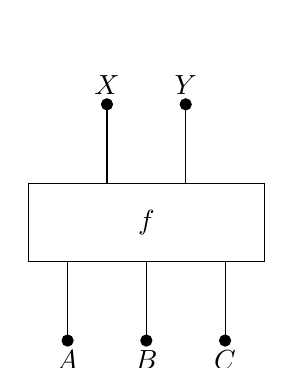
\begin{tikzpicture}
    \filldraw[black] (-0.5,0) circle (2pt) node[anchor=south]{$X$};
    \filldraw[black] (0.5,0) circle (2pt) node[anchor=south]{$Y$};
    \draw (-0.5, 0) -- (-0.5, -1);
    \draw (0.5, 0) -- (0.5, -1);
    \draw (-1.5, -1) -- (-1.5, -2) -- (1.5, -2) -- (1.5, -1) -- cycle;
    \draw (-1, -2) -- (-1, -3);
    \draw (0, -2) -- (0, -3);
    \draw (1, -2) -- (1, -3);
    \draw (0,-1.5) node{$f$};
    \filldraw[black] (-1,-3) circle (2pt) node[anchor=north]{$A$};
    \filldraw[black] (0,-3) circle (2pt) node[anchor=north]{$B$};
    \filldraw[black] (1,-3) circle (2pt) node[anchor=north]{$C$};
  \end{tikzpicture}
\end{center}

We can compose morphisms by concatenating their diagrams.
\begin{center}
  \begin{tikzpicture}
    \filldraw[black] (-0.5,0) circle (2pt) node[anchor=south]{$X$};
    \filldraw[black] (0.5,0) circle (2pt) node[anchor=south]{$Y$};
    \draw (-0.5, 0) -- (-0.5, -1);
    \draw (0.5, 0) -- (0.5, -1);
    \draw (-1.5, -1) -- (-1.5, -2) -- (1.5, -2) -- (1.5, -1) -- cycle;
    \draw (-1, -2) -- (-1, -3);
    \draw (0, -2) -- (0, -3);
    \draw (1, -2) -- (1, -3);
    \draw (0,-1.5) node{$f$};
    \draw (-1.5, -4) -- (-1.5, -3) -- (1.5, -3) -- (1.5, -4) -- cycle;
    \draw (0,-3.5) node{$g$};
    \draw (0, -4) -- (0, -5);
    \filldraw[black] (0, -5) circle (2pt) node[anchor=north]{$Z$};
  \end{tikzpicture}
\end{center}

In a braided monoidal category, we require that for any two objects $X$ and $Y$ we have an isomorphism $\gamma_{XY}\colon X \otimes Y \to Y \otimes X$, which we draw like this.

\begin{center}
  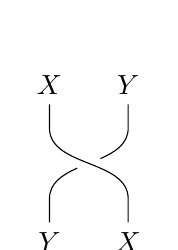
\begin{tikzpicture}
    \braid (braid) s_1;
    \node[at=(braid-1-s), anchor=south]{$X$};
    \node[at=(braid-2-s), anchor=south]{$Y$};
    \node[at=(braid-1-e), anchor=north]{$X$};
    \node[at=(braid-2-e), anchor=north]{$Y$};
  \end{tikzpicture}
\end{center}

Since $\gamma_{AB}$ is an isomorphism, it has an inverse $\gamma_{AB}^{-1}$ (not necessarily equal to $\gamma_{BA}$!) which we draw like this.

\begin{center}
  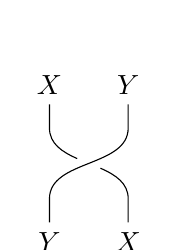
\begin{tikzpicture}
    \braid (braid) s_{1}^{-1};
    \node[at=(braid-1-s), anchor=south]{$X$};
    \node[at=(braid-2-s), anchor=south]{$Y$};
    \node[at=(braid-1-e), anchor=north]{$X$};
    \node[at=(braid-2-e), anchor=north]{$Y$};
  \end{tikzpicture}
\end{center}

The idea of a braided monoidal category is that we want to take these pictures seriously: we want two expressions involving repeated applications of the $\gamma_{\cdot\cdot}$ and their inverses to be equivalent if and only if the braid diagrams representing them are homotopic. Thus we want, for example,
\begin{equation*}
  \gamma_{XY} \circ \gamma_{YZ} \circ \gamma_{XY} =  \gamma_{YZ} \circ \gamma_{XY} \circ \gamma_{YZ}
\end{equation*}
since
\begin{center}
  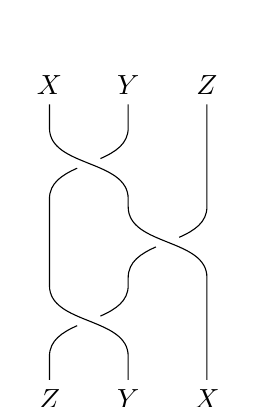
\begin{tikzpicture}
    \braid (braid) s_1 s_{2} s_{1};
    \node[at=(braid-1-s), anchor=south]{$X$};
    \node[at=(braid-2-s), anchor=south]{$Y$};
    \node[at=(braid-3-s), anchor=south]{$Z$};
    \node[at=(braid-1-e), anchor=north]{$X$};
    \node[at=(braid-2-e), anchor=north]{$Y$};
    \node[at=(braid-3-e), anchor=north]{$Z$};
  \end{tikzpicture}
\end{center}

is homotopic to

\begin{center}
  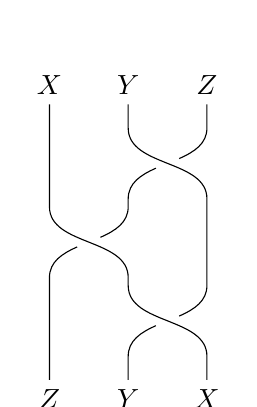
\begin{tikzpicture}
    \braid (braid) s_2 s_{1} s_{2};
    \node[at=(braid-1-s), anchor=south]{$X$};
    \node[at=(braid-2-s), anchor=south]{$Y$};
    \node[at=(braid-3-s), anchor=south]{$Z$};
    \node[at=(braid-1-e), anchor=north]{$X$};
    \node[at=(braid-2-e), anchor=north]{$Y$};
    \node[at=(braid-3-e), anchor=north]{$Z$};
  \end{tikzpicture}.
\end{center}

A digression into the theory of braid groups would take us too far afield. The punchline is that to guarantee that all such compositions involving the $\gamma$ are identified in the correct way, we must define braided monoidal categories as follows.

\begin{definition}[braided monoidal category]
  \label{def:braidedmonoidalcategory}
  A catgory $\mathsf{C}$ with monoidal structure $(\otimes, 1, \alpha, \lambda, \rho)$ is \defn{braided} if for every two objects $A$ and $B \in \Obj(\mathsf{C})$, there is an isomorphism $\gamma_{A,B}\colon A \otimes B \to B \otimes A$ such that the following \emph{hexagon diagrams} commute.
  \begin{equation*}
    \begin{tikzcd}
      & A \otimes (B \otimes C) \arrow[r, "{\gamma_{A, B \otimes C}}"] & (B \otimes C) \otimes A \arrow[dr, "\alpha_{BCA}"] & \\
      (A \otimes B) \otimes C \arrow[ur, "\alpha_{ABC}"] \arrow[dr, swap, "\gamma_{AB} \otimes 1"] & & & B \otimes (C \otimes A) \\
      & (B \otimes A) \otimes C \arrow[r, swap, "\alpha_{BAC}"] & (B \otimes A) \otimes C \arrow[ur, swap, "1 \otimes \gamma"]
    \end{tikzcd}
  \end{equation*}
  \begin{equation*}
    \begin{tikzcd}
      & (A \otimes B) \otimes C \arrow[r, "{\gamma_{A \otimes B, C}}"] & C \otimes (A \otimes B) \arrow[dr, "\alpha^{-1}_{CAB}"] \\
      A \otimes (B \otimes C) \arrow[ur, "\alpha_{ABC}^{-1}"] \arrow[dr, swap, "1 \otimes \gamma_{BC}"] & & & (C \otimes A) \otimes B \\
      & A \otimes (C \otimes B) \arrow[r, swap, "\alpha^{-1}_{ACB}"] & (A \otimes C) \otimes B \arrow[ur, swap, "\gamma_{AC} \otimes 1"]
    \end{tikzcd} 
  \end{equation*}
  The collection of such $\gamma$ form a natural isomorphism betweem the bifunctors 
  \begin{equation*}
    (A, B) \mapsto A \otimes B\qquad\text{and}\qquad (A,B) \mapsto B \otimes A,
  \end{equation*}
  and is called a \defn{braiding}.
\end{definition}

\begin{definition}[braided monoidal functor]
  \label{def:braidedmonoidalfunctor}
  A lax monoidal functor $(\mathcal{F}, \Phi, \phi)$ (\hyperref[def:monoidalfunctor]{Definition \ref*{def:monoidalfunctor}}) is \defn{braided monoidal} if it makes the following diagram commute.
  \begin{equation*}
    \begin{tikzcd}[row sep=huge, column sep=huge]
      \mathcal{F}(x) \otimes \mathcal{F}(y)
      \arrow[r, "{\gamma_{\mathcal{F}(x), \mathcal{F}(y)}}"]
      \arrow[d, swap, "{\Phi_{x,  y}}"]
      & \mathcal{F}(y) \otimes \mathcal{F}(x)
      \arrow[d, "{\Phi_{x, y}}"]
      \\
      \mathcal{F}(x \otimes y)
      \arrow[r, "{\mathcal{F}(\gamma_{x, y})}"]
      & \mathcal{F}(y \otimes x)
    \end{tikzcd}
  \end{equation*}
  \begin{note}
    There are no extra conditions imposed on a monoidal natural transformation to turn it into a braided natural transformation. 
  \end{note}
\end{definition}

\subsection{Symmetric monoidal categories}
Until now, we have been calling the bifunctor $\otimes$ in \hyperref[def:monoidalcategory]{Definition \ref*{def:monoidalcategory}} a tensor product. This has been an abuse of terminology: in general, one defines tensor products not to be those bifunctors which come from any monoidal category, but only those which come from \emph{symmetric} monoidal categories. We will define these shortly.

Conceptually, passing from the definition of a braided monoidal category to that of a symmetric monoidal category is rather simple. One only requires that for any two objects $A$ and $B$, $\gamma_{BA} = \gamma_{AB}^{-1}$, i.e. $\gamma_{BA} \circ \gamma_{AB} = 1_{A \otimes B}$.

We can interpret this nicely in terms of our braid diagrams. We can draw $\gamma_{BA} \circ \gamma_{AB}$ like this.

\begin{center}
  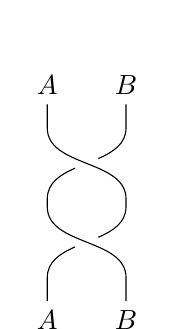
\begin{tikzpicture}
    \braid (braid) s_1 s_1;
    \node[at=(braid-1-s), anchor=south]{$A$};
    \node[at=(braid-2-s), anchor=south]{$B$};
    \node[at=(braid-1-e), anchor=north]{$A$};
    \node[at=(braid-2-e), anchor=north]{$B$};
  \end{tikzpicture}
\end{center}

The requirement that this must be homotopic to the identity transformation
\begin{center}
  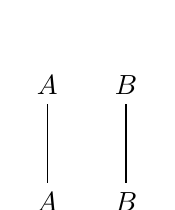
\begin{tikzpicture}
    \draw (0,0) node[anchor=south]{$A$} -- (0,-1) node[anchor=north]{$A$};
    \draw (1,0) node[anchor=south]{$B$} -- (1,-1) node[anchor=north]{$B$};
  \end{tikzpicture}
\end{center}

can be expressed by making the following rule: in a \emph{symmetric} monoidal category, we don't care about the difference between undercrossings and overcrossings:
\begin{center}
  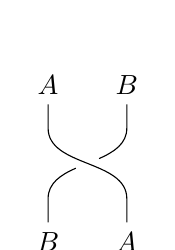
\begin{tikzpicture}
    \braid (braid) s_1;
    \node[at=(braid-1-s), anchor=south]{$A$};
    \node[at=(braid-2-s), anchor=south]{$B$};
    \node[at=(braid-1-e), anchor=north]{$A$};
    \node[at=(braid-2-e), anchor=north]{$B$};
  \end{tikzpicture}
  \qquad = \qquad
  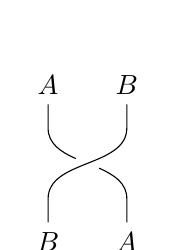
\begin{tikzpicture}
    \braid (braid) s_1^{-1};
    \node[at=(braid-1-s), anchor=south]{$A$};
    \node[at=(braid-2-s), anchor=south]{$B$};
    \node[at=(braid-1-e), anchor=north]{$A$};
    \node[at=(braid-2-e), anchor=north]{$B$};
  \end{tikzpicture}
\end{center}

Then we can exchange the diagram representing $\gamma_{BA} \circ \gamma_{AB}$ for

\begin{center}
  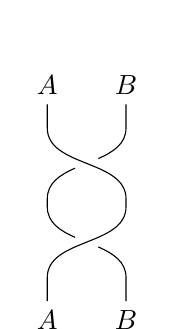
\begin{tikzpicture}
    \braid (braid) s_1 s_1^{-1};
    \node[at=(braid-1-s), anchor=south]{$A$};
    \node[at=(braid-2-s), anchor=south]{$B$};
    \node[at=(braid-1-e), anchor=north]{$A$};
    \node[at=(braid-2-e), anchor=north]{$B$};
  \end{tikzpicture}
\end{center}
which is clearly homotopic to the identity transformation on $A \otimes B$.

\begin{definition}[symmetric monoidal category]
  \label{def:symmetricmonoidalcategory}
  Let $\mathsf{C}$ be a braided monoidal category with braiding $\gamma$. We say that $\mathsf{C}$ is a \defn{symmetric monoidal category} if for all $A$, $B \in \Obj(\mathsf{C})$, $\gamma_{BA} \circ \gamma_{AB} = 1_{A \otimes B}$. A braiding $\gamma$ which satisfies such a condition is called \defn{symmetric}.
\end{definition}

\begin{note}
  There are no extra conditions imposed on a monoidal natural transformation to turn it into a symmetric natural transformation. 
\end{note}
\section{Enriched categories}
The rough idea of enrichment is this: we have a category $\mathsf{C}$, and we would like to treat the hom-sets $\Hom_{\mathsf{C}}(A, B)$ as living in some category $\mathsf{K}$, not necessarily $\mathsf{Set}$. This is a common occurrence; often morphisms between structures inherit properties from the structures themselves. 
\begin{itemize}
  \item In $\mathsf{Ab}$, the endomorphisms $\End_{\mathsf{Ab}}(G) = \Hom_{\mathsf{Ab}}(G, G)$ naturally have a ring structure: we can define addition pointwise
    \begin{equation*}
      (\alpha + \beta)(g) = \alpha(g) + \beta(g),
    \end{equation*}
    multiplication by composition
    \begin{equation*}
      (\alpha \circ \beta)(g) = \alpha(\beta(g)).
    \end{equation*}
    These operatations satisfy the ring axioms. Therefore, we would like to view the endomorphisms in $\mathsf{Ab}$ as living not just in $\mathsf{Set}$, but in $\mathsf{Ring}$.

  \item In $\mathsf{Vect}_{k}$, the linear maps between vector spaces inherit the structure of a vector space: we can define addition and scalar multiplication by
    \begin{equation*}
      (A + B)v = Av + Bv\qquad\text{and }(\lambda A)v = \lambda(Av).
    \end{equation*}
    Therefore, we would like to view the morphisms in $\mathsf{Vect}_{k}$ as living in $\mathsf{Vect}_{k}$
\end{itemize}
If we are to replace hom-sets with more general objects belonging to a generic enriching category, we need to make sure that the enriching category has enough structure to mimic the behavior of the hom-sets. In particular, we need a way to compose morphisms. This is not as trivial as it sounds; we are in general not allowed to talk about the elements of an object in a category, so we need to replace our definition of the composition of morphisms as a set map $\Hom_{\mathsf{C}}(B, C) \times \Hom_{\mathsf{C}}(A, B) \to \Hom_{\mathsf{C}}(A, C)$ with something that doesn't know about the elements of the hom-sets. The correct way of doing this is with a monoidal structure.

\begin{definition}[enriched category]
  \label{def:enrichedcategory}
  Let $\mathsf{K}$ be a monoidal category with monoidal structure $(\times, 1, \alpha, \lambda, \rho)$. A (small) \defn{$\mathsf{K}$-enriched category} $\mathsf{C}$ consists of the following. 
  \begin{itemize}
    \item A set $\Obj(\mathsf{C})$ of objects

    \item For each ordered pair $(A, B)$ of objects of $\mathsf{C}$, an object $\Hom_{\mathsf{C}}(A, B) \in \Obj(\mathsf{K})$ (also written $\mathsf{C}(A, B)$) called the \emph{hom-object},

    \item For each ordered triple $(A, B, C)$ of objects of $\mathsf{C}$ a morphism $\circ_{A, B, C}: \Hom_{\mathsf{C}}(B, C) \times \Hom_{\mathsf{C}}(A, B) \to \Hom_{\mathsf{C}}(A, C)$ called the \emph{composition morphism}

    \item for each object $A \in \Obj(\mathsf{C})$ a morphism $j_{A}: 1 \to \Hom_{\mathsf{C}}(A, A)$ called the identity element
  \end{itemize}
  such that the following diagrams commute.
  \begin{equation*}
    \begin{tikzcd}[row sep=large]
      (\mathsf{C}(C, D) \times \mathsf{C}(B, C)) \times \mathsf{C}(A, B)
      \arrow[rr, "\alpha"]
      \arrow[d, swap, "\circ \times 1"]
      & & \mathsf{C}(C, D) \times (\mathsf{C}(B, C) \times \mathsf{C}(A, B))
      \arrow[d, "1 \times \circ"]
      \\
      \mathsf{C}(B, D) \times \mathsf{C}(A, B)
      \arrow[r, "\circ"]
      & \mathsf{C}(A, D)
      & \mathsf{C}(C, D) \times \mathsf{C}(A, C)
      \arrow[l, swap, "\circ"]
    \end{tikzcd}
  \end{equation*}
  \begin{equation*}
    \begin{tikzcd}[row sep=large]
      \mathsf{C}(B, B) \times \mathsf{C}(A, B)
      \arrow[r, "\circ"]
      & \mathsf{C}(A, B)
      & \mathsf{C}(A, B) \times \mathsf{C}(A, A)
      \arrow[l, swap, "\circ"]
      \\
      1 \times \mathsf{C}(A, B)
      \arrow[u, "j \times 1"]
      \arrow[ur, swap, "\lambda"]
      & & \mathsf{C}(A, B) \times 1
      \arrow[ul, "\rho"]
      \arrow[u, swap, "1 \times j"]
    \end{tikzcd}
  \end{equation*}
  The first diagram enforces associativity; the second ensures that composition is unital.
\end{definition}

\section{Limits and colimits}
As we have seen, one often gets categorical concepts by `categorifying' concepts from set theory. One example of this is the notion of a \emph{diagram}, which is the categorical generalization of an indexed family.

\begin{definition}[indexed family]
  \label{def:indexedfamily}
  Let $J$ and $X$ be sets. A \defn{family of elements in $X$ indexed by $J$} is a function
  \begin{equation*}
    x\colon J \to X;\qquad j \mapsto x_{j}.
  \end{equation*}
\end{definition}

To categorify this, one considers a functor from one category $\mathsf{J}$, called the \emph{index category}, to another category $\mathsf{C}$. Using a functor from a category instead of a function from a set allows us to index the morphisms as well as the objects. 

\begin{definition}[diagram]
  \label{def:diagram}
  Let $\mathsf{J}$ and $\mathsf{C}$ be categories. A \defn{diagram} of type $\mathsf{J}$ in $\mathsf{C}$ is a covariant functor
  \begin{equation*}
    \mathcal{D}\colon \mathsf{J} \rightsquigarrow \mathsf{C}.
  \end{equation*}
\end{definition}

One thinks of the functor $\mathcal{D}$ embedding the index category $\textsf{J}$ into $\mathsf{C}$.

\begin{definition}[cone]
  \label{def:cone}
  Let $\mathsf{C}$ be a category, $\mathsf{J}$ an index category, and $\mathcal{D}\colon \mathsf{J} \rightsquigarrow \mathsf{C}$ be a diagram. Let $\mathsf{1}$ be the category with one object and one morphism (\hyperref[eg:categorywithoneobject]{Example \ref*{eg:categorywithoneobject}}) and $\mathcal{F}_{X}$ the functor $1 \rightsquigarrow \mathsf{C}$ which picks out $X \in \Obj(\mathsf{C})$ (see e.g. \hyperref[eg:functorfrom1category]{Example \ref*{eg:functorfrom1category}}). Let $\mathcal{K}$ be the unique functor $\mathsf{J} \rightsquigarrow \mathsf{1}$.
  \begin{equation*} 
    \begin{tikzcd}
      \mathsf{1}
      \arrow[rd, rightsquigarrow, "\mathcal{F}_{X}"]
      \\
      \mathsf{J}
      \arrow[u, rightsquigarrow, "\mathcal{K}"]
      \arrow[r, rightsquigarrow, "\mathcal{D}"]
      & \mathsf{C}
    \end{tikzcd}
  \end{equation*}
  A \defn{cone} of shape $\mathsf{J}$ from $X$ is an object $X \in \Obj(\mathsf{C})$ together with a natural transformation
  \begin{equation*}
    \varepsilon\colon \mathcal{F}_{X} \circ \mathcal{K} \Rightarrow \mathcal{D}.
  \end{equation*}

  That is to say, a cone to $\mathsf{J}$ is an object $X \in \Obj(\mathsf{C})$ together with a family of morphisms $\Phi_{A}\colon X \to \mathcal{F}(A)$ (one for each $A \in \Obj(\mathsf{J})$) such that for all $A$, $B \in \Obj(\mathsf{J})$ and all $f\colon A \to B$ the following diagram commutes.
  \begin{equation*}
    \begin{tikzcd}[column sep=tiny]
      & X
      \arrow[dl, swap, "\Phi_{A}"]
      \arrow[dr, "\Phi_{B}"]
      \\
      \mathcal{F}(A)
      \arrow[rr, "\mathcal{F}(f)"]
      & & \mathcal{F}(B)
    \end{tikzcd}
  \end{equation*}
\end{definition}

\begin{note}
  \label{note:alternatedefinitionofcone}
  Here is an alternate definition. Let $\Delta$ be the functor $\mathsf{C} \rightsquigarrow [\mathsf{J}, \mathsf{C}]$ (the category of functors $\mathsf{J} \rightsquigarrow \mathsf{C}$, see TODO) which assigns to each object $X \in \Obj(\mathsf{C})$ the constant functor $\Delta_{X}: \mathsf{J} \rightsquigarrow \mathsf{C}$, i.e. the functor which maps every object of $\mathsf{J}$ to $X$ and every morphism to $1_{X}$. A cone over $\mathcal{D}$ is then an object in the comma category (\hyperref[def:commacategory]{Definition \ref*{def:commacategory}}) $(\Delta \downarrow \mathcal{D})$ given by the diagram
  \begin{equation*}
    \begin{tikzcd}
      \mathsf{C}
      \arrow[r, rightsquigarrow, "\Delta"]
      & {[\mathsf{J}, \mathsf{C}]}
      & \mathsf{1}
      \arrow[l, swap, rightsquigarrow, "\mathcal{F}_{D}"]
    \end{tikzcd}.
  \end{equation*}

  The objects of this category are pairs $(X, f)$, where $X \in \Obj(\mathsf{C})$ and $f\colon \Delta(X) \to \mathcal{D}$; that is to say, $f$ is a natural transformation $\Delta_{X} \Rightarrow \mathcal{D}$.

\end{note}
This allows us to make the following definition. 

\begin{definition}[category of cones over a diagram]
  \label{def:categoryofconesoveradiagram}
  Let $\mathsf{C}$ be a category, $\mathsf{J}$ an index category, and $\mathcal{D}\colon \mathsf{J} \rightarrow \mathsf{C}$ a diagram. The \defn{category of cones over $\mathcal{D}$} is the category $(\Delta \downarrow \mathcal{D})$.
\end{definition} 

\begin{note}
  The previous definition not only reiterates what cones look like, but even prescribes what morphisms between cones look like. Let $(X, \Phi)$ be a cone over a diagram $\mathcal{D}\colon \mathsf{J} \rightsquigarrow \mathsf{C}$, i.e.
  \begin{itemize}
    \item an object in the category $(\Delta \downarrow \mathcal{D})$, i.e.
    \item a pair $(X, \Phi)$, where $X \in \Obj(\mathsf{C})$ and $\Phi\colon \Delta_{X} \Rightarrow \mathcal{D}$ is a natural transformation, i.e.
    \item for each $J \in \Obj(\mathsf{J})$ a morphism $\Phi_{J}\colon X \to \mathcal{D}(J)$ such that for any other object $J' \in \Obj(\mathsf{J})$ and any morphism $f\colon J \to J'$ the following diagram commutes.
      \begin{equation*}
        \begin{tikzcd}
          & X
          \arrow[ld, swap, "\Phi_{J}"]
          \arrow[rd, "\Phi_{J'}"]
          \\
          \mathcal{D}(J)
          \arrow[rr, "\mathcal{D}(f)"]
          & & \mathcal{D}(J')
        \end{tikzcd}
      \end{equation*}
  \end{itemize}
  This agrees with our previous definition of a cone.

  Let $(Y, \Gamma)$ be another cone over $\mathcal{D}$. Then a morphism $\Xi\colon (X, \Phi) \to (Y, \Gamma)$ is 
  \begin{itemize}
    \item a morphism $\Xi \in \Hom_{(\Delta \downarrow \mathcal{D})}((X, \Phi), (Y, \Gamma))$, i.e.
    \item a natural transformation $\Xi\colon \Delta_{X} \Rightarrow \Delta_{Y}$ (i.e. a morphism $\Delta_{X} \to \Delta_{Y}$ in the category $[\mathsf{J}, \mathsf{C}]$) such that the diagram
      \begin{equation*}
        \begin{tikzcd}
          \Delta_{X}
          \arrow[rr, Rightarrow, "\Xi"]
          \arrow[rd, Rightarrow, "\Phi"]
          & &  \Delta_{Y}
          \arrow[ld, swap, Rightarrow, "\Gamma"]
          \\
          & \mathcal{D}
        \end{tikzcd}
      \end{equation*}
      commutes, i.e.
    \item a morphism $\xi\colon X \to Y$ such that for each $J \in \Obj(\mathsf{J})$, the diagram
      \begin{equation*}
        \begin{tikzcd}
          X
          \arrow[rr, "\xi"]
          \arrow[rd, "\Phi_{J}"]
          & & Y
          \arrow[ld, swap, "\Gamma_{J}"]
          \\
          & \mathcal{D}(J)
        \end{tikzcd}
      \end{equation*}
      commutes.
  \end{itemize}
\end{note}

Cocones are the dual notion to cones. We make the following definition.
\begin{definition}[cocone]
  \label{def:cocone}
  A \defn{cocone over a diagram $\mathcal{D}$} is an object in the comma category $(\mathcal{D} \downarrow \Delta)$.
\end{definition}

\begin{definition}[category of cocones]
  \label{def:categoryofcocones}
  The \defn{category of cocones over a diagram $\mathcal{D}$} is the category $(\mathcal{D} \downarrow \Delta)$.
\end{definition}

The categorical definitions of cones and cocones allow us to define limits and colimits succinctly.
\begin{definition}[limits, colimits]
  \label{def:limitscolimits}
  A \defn{limit} of a diagram $\mathcal{D}\colon \mathsf{J} \rightsquigarrow \mathsf{C}$ is a final object in the category $(\Delta \downarrow \mathcal{D})$. A \defn{colimit} is an initial object in the category $(\mathcal{D} \downarrow \Delta)$.
\end{definition}

\begin{note}
  The above definition of a limit unwraps as follows. The limit of a diagram $\mathcal{D}\colon \mathsf{J} \rightsquigarrow \mathsf{C}$ is a cone $(X, \Phi)$ over $\mathcal{D}$ such that for any other cone $(Y, \Gamma)$ over $\mathcal{D}$, there is a unique map $\xi\colon Y \to X$ such that for each $J \in \Obj(\mathsf{J})$, the following diagram commutes.
  \begin{equation*}
    \begin{tikzcd}[column sep=tiny]
      Y
      \arrow[rr, "\xi"]
      \arrow[dr, swap, "\Gamma_{J}"]
      & & X
      \arrow[dl, "\Phi_{J}"]
      \\
      & \mathcal{D}(J)
    \end{tikzcd}
  \end{equation*}
\end{note} 

\begin{example}[equalizer]
  Let $\mathsf{J}$ be the category with objects and morphisms as follows. (The necessary identity arrows are omitted.)
  \begin{equation*}
    \begin{tikzcd}
      J
      \arrow[r, shift left, "1"]
      \arrow[r, shift right, swap, "2"]
      & J'
    \end{tikzcd}
  \end{equation*}

  A diagram $\mathcal{D}$ of shape $\mathsf{J}$ in some category $\mathsf{C}$ looks like the following (the identity morphisms don't tell us anything, so we don't draw them).
  \begin{equation*}
    \begin{tikzcd}
      A 
      \arrow[r, shift left, "f"]
      \arrow[r, shift right, swap, "g"]
      & B
    \end{tikzcd}
  \end{equation*}

  The \defn{equalizer} of $f$ and $g$ is the limit of the diagram $\mathcal{D}$; that is to say, it is an object $\mathrm{eq} \in \Obj(\mathsf{C})$ and a morphism $e\colon \mathrm{eq} \to A$
  \begin{equation*}
    \begin{tikzcd}
      \mathrm{eq}
      \arrow[r, "e"]
      & A
      \arrow[r, shift left, "f"]
      \arrow[r, shift right, swap, "g"]
      & B
    \end{tikzcd}
  \end{equation*}
  such that for any \emph{other} object $Z$ and morphism $i\colon Z \to A$, there is a unique morphism $e\colon Z \to \mathrm{eq}$ making the following diagram commute.
  \begin{equation*}
    \begin{tikzcd}
      Z 
      \arrow[d, swap, dashed, "\exists! u"]
      \arrow[dr, "i"]
      \\
      \mathrm{eq}
      \arrow[r, swap, "e"]
      & A
      \arrow[r, shift left, "f"]
      \arrow[r, shift right, swap, "g"]
      & B
    \end{tikzcd}
  \end{equation*}

  So what does it mean for the above diagram to commute in, say, $\mathsf{Set}$? We need $(f \circ e)(x) = (g \circ e)(x)$ for all $x \in \mathrm{eq}$. That is, once we have been mapped by $e$ into $A$, we need to be taken to the same place by $f$ and $g$. The range of $e$ must lie entirely within the set 
\end{example}

\section{Kernels and cokernels}
In what follows, $\mathsf{C}$ will be a category and $A$, $B$, etc. objects in $\Obj(\mathsf{C})$.
\subsection{Kernels}
\begin{definition}[pullback]
  \label{def:pullback}
  Let $f$, $g$ be morphisms as follows.
  \begin{equation*}
    \begin{tikzcd}
      & B \arrow[d, "g"] \\
      A \arrow[r, swap, "f"] & C
    \end{tikzcd}
  \end{equation*}
  A \defn{pullback of $f$ along $g$} (also called a pullback of $g$ over $f$, sometimes notated $A \times_{C} B$) is a commuting square 
  \begin{equation*}
    \begin{tikzcd}
      U \arrow[r, "q"] \arrow[d, "p", swap] & B \arrow[d, "g"] \\
      A \arrow[r, swap, "f"] & C
    \end{tikzcd}
  \end{equation*}
  such that for any other commuting square
  \begin{equation*}
    \begin{tikzcd}
      V \arrow[r, "t"] \arrow[d, "s", swap] & B \arrow[d, "g"] \\
      A \arrow[r, swap, "f"] & C
    \end{tikzcd}
  \end{equation*}
  there is a unique morphism $h\colon V \to U$ such that the diagram
  \begin{equation*}
    \begin{tikzcd}
      V \arrow[rrd, bend left, "t"] \arrow[rd, dashed, "\exists!h"] \arrow[rdd, bend right, swap, "s"] &   &  \\
      & U \arrow[r, "q"] \arrow[d, swap, "p"] & B \arrow[d, "g"] \\
      & A \arrow[r, swap, "f"] & C
    \end{tikzcd}
  \end{equation*}
\end{definition}
\begin{note}
  Here is another definition: the pullback $A \times_{C} B$ is the limit of the diagram
  \begin{equation*}
    \begin{tikzcd}
      & B
      \arrow[d, "g"]
      \\
      A
      \arrow[r, swap, "f"]
      & C
    \end{tikzcd}
  \end{equation*}

  This might at first seem odd; after all, don't we also need an arrow $A \times_{C} B \to C$? But this arrow is completely determined by the commutativity conditions, so it is superfluous.
\end{note}
\begin{example}
  In $\mathsf{Set}$, $U$ is given (up to unique isomorphism) by 
  \begin{equation*}
    U = \left\{ (a,b) \in A \times B \,\big|\, f(a) = g(b) \right\}.
  \end{equation*}

  The morphisms $p$ and $q$ are given by the projections $p(a,b) = a$, $q(a,b) = b$.

  To see that this really does satisfy the universal property, consider any other set $V$ and functions $s\colon V \to A$ and $t\colon V \to B$ making the above diagram commute. Then for all $v \in V$, $f(s(v)) = t(g(v))$.

  Now consider the map $V \to U$ sending $v$ to $(s(v), t(v))$. This certainly makes the above diagram commute; furthermore, any other map from $V$ to $U$ would not make the diagram commute. Thus $U$ and $h$ together satisfy the universal property.
\end{example}

\begin{definition}[kernel of a morphism]
  \label{def:kernelofmorphism}
  Let $\mathsf{C}$ be a category with an initial object (\hyperref[def:initialfinalzeroobject]{Definition \ref*{def:initialfinalzeroobject}}) $0$ and pullbacks. The \defn{kernel} $\ker(f)$ of a morphism $f\colon A \to B$ is the pullback along $f$ of the unique morphism $0 \to B$.
  \begin{equation*}
    \begin{tikzcd}
      \ker(f) \arrow[d, swap, "\iota"] \arrow[r] & 0 \arrow[d] \\
      A \arrow[r, "f"] & B
    \end{tikzcd}
  \end{equation*}

  That is to say, the kernel of $f$ is a pair $(\ker(f), \iota)$, where $\ker(f) \in \Obj(\mathsf{C})$ and $\iota\colon \ker(f) \to A$ which satisfies the above universal property.
\end{definition}

\begin{note}
  Although the kernel of a morphism $f$ is a pair $(\ker(f), \iota)$ as described above, we will sometimes sloppily say that the object $\ker(f)$ is the kernel of $f$, especially when the the morphism $\iota$ is obvious or understood.
\end{note}

\begin{example}
  In $\mathsf{Vect}_{k}$, the initial object is the zero vector space $\{0\}$. For any vector spaces $V$ and $W$ and any linear map $f\colon V \to W$, the kernel of $f$ is the pair $(\ker(f), \iota)$ where $\ker(f)$ is the vector space  
  \begin{equation*}
    \ker(f) = \left\{ v \in V \,\big|\, f(v) = 0 \right\}
  \end{equation*}
  and $\iota$ is the obvious injection $\ker(f) \to V$.
\end{example}

\begin{lemma}
  \label{lemma:canonicalinjectionismono}
  Let $f\colon A \to B$, and let $(\iota, \ker(f))$ be the kernel of $f$. Then $\iota$ is a monomorphism (\hyperref[def:monomorphism]{Definition \ref*{def:monomorphism}}).
\end{lemma}
\begin{proof}
  Suppose we have an object $Z \in \Obj(\mathsf{C})$ and two morphisms $g_{1}$, $g_{2}\colon Z \to \ker(f)$. We have the following diagram.
  \begin{equation*}
    \begin{tikzcd}
      Z
      \arrow[rd, shift left, "g_{1}"]
      \arrow[rd, shift right, swap, "g_{2}"]
      \\
      & \ker(f)
      \arrow[r]
      \arrow[d, "\iota"]
      & 0
      \arrow[d]
      \\
      & A
      \arrow[r, "f"]
      & B
    \end{tikzcd}
  \end{equation*}
  Further suppose that $\iota \circ g_{1} = \iota \circ g_{2}$.
  \begin{equation*}
    \begin{tikzcd}
      Z
      \arrow[rd, shift left, "g_{1}"]
      \arrow[rd, shift right, swap, "g_{2}"]
      \arrow[rrd, bend left]
      \arrow[rdd, bend right, swap, "\iota \circ g_{1} = \iota \circ g_{2}"]
      \\
      & \ker(f)
      \arrow[r]
      \arrow[d, swap, "\iota"]
      & 0
      \arrow[d]
      \\
      & A
      \arrow[r, "f"]
      & B
    \end{tikzcd}
  \end{equation*}

  Now pretend that we don't know about $g_{1}$ and $g_{2}$.
  \begin{equation*}
    \begin{tikzcd}
      Z
      \arrow[rrd, bend left]
      \arrow[rdd, bend right, swap, "\iota \circ g_{1} = \iota \circ g_{2}"]
      \\
      & \ker(f)
      \arrow[r]
      \arrow[d, swap, "\iota"]
      & 0
      \arrow[d]
      \\
      & A
      \arrow[r, "f"]
      & B
    \end{tikzcd}
  \end{equation*}

  The universal property for kernels tells us that there is a unique map $Z \to \ker(f)$ making the above diagram commute. But since $g_{1}$ and $g_{2}$ both make the diagram commute, $g_{1}$ and $g_{2}$ must be the same map, i.e. $g_{1} = g_{2}$.
\end{proof}

\subsection{Cokernels}
Pushouts are the dual notion to pullbacks.
\begin{definition}[pushouts]
  \label{def:pushout}
  Let $f$, $g$ be morphisms as follows.
  \begin{equation*}
    \begin{tikzcd}
      C \arrow[r, "g"] \arrow[d, swap, "f"] & B \\
      A
    \end{tikzcd}
  \end{equation*}
  The \defn{pushout of $f$ along $g$} (or $g$ along $f$) is a commuting square
  \begin{equation*}
    \begin{tikzcd}
      C \arrow[r, "g"] \arrow[d, swap, "f"] & B \arrow[d, "q"] \\
      A \arrow[r, swap, "p"] & U
    \end{tikzcd}
  \end{equation*}
  such that for any other commuting square
  \begin{equation*}
    \begin{tikzcd}
      C \arrow[r, "g"] \arrow[d, swap, "f"] & B \arrow[d, "t"] \\
      A \arrow[r, swap, "s"] & V
    \end{tikzcd}
  \end{equation*}
  there exists a unique morphism $h\colon U \to V$ such that the diagram 
  \begin{equation*}
    \begin{tikzcd}
      C \arrow[r, "g"] \arrow[d, swap, "f"] & B \arrow[d, "q"] \arrow[ddr, bend left, "t"] & \\
      A \arrow[drr, bend right, swap, "s"] \arrow[r, swap, "p"] & U \arrow[dr, dashed, "\exists!h"] & \\
      & & V
    \end{tikzcd}
  \end{equation*}
  commutes.
\end{definition}

\begin{note}
  As with pullbacks, we can also define a pushout as the colimit of the following diagram.
  \begin{equation*}
    \begin{tikzcd}
      C \arrow[r, "g"] \arrow[d, swap, "f"] & B \\
      A
    \end{tikzcd}
  \end{equation*}
\end{note}

\begin{example}
  Let us construct the pushout in $\mathsf{Set}$. If we ignore the object $C$ and the morphisms $f$ and $g$, we discover that $U$ must satisfy the universal property of the coproduct of $A$ and $B$. 
  \begin{equation*}
    \begin{tikzcd}
      & B \arrow[d, "q"] \arrow[ddr, bend left, "t"] & \\
      A \arrow[drr, bend right, swap, "s"] \arrow[r, swap, "p"] & U \arrow[dr, dashed, "\exists!h"] & \\
      & & V
    \end{tikzcd}
  \end{equation*}
  Let us therefore make the ansatz that $U = A \amalg B = A \sqcup B$ and see what happens when we add $C$, $f$, and $g$ back in. 
  \begin{equation*}
    \begin{tikzcd}
      C \arrow[r, "g"] \arrow[d, swap, "f"] & B \arrow[d, "q"] \arrow[ddr, bend left, "t"] & \\
      A \arrow[drr, bend right, swap, "s"] \arrow[r, swap, "p"] & U \arrow[dr, dashed, "\exists!h"] & \\
      & & V
    \end{tikzcd}
  \end{equation*}

  In doing so, we find that the square $A$-$C$-$B$-$U$ must also commute, i.e. we must have that $(q \circ g) (c) = (p \circ f)(c)$ for all $c \in C$. Since $p$ and $q$ are just inclusions, we see that
  \begin{equation*}
    U = A \amalg B / \sim,
  \end{equation*}
  where $\sim$ is the equivalence relation generated by the relations $f(c) \sim g(c)$ for all $c\in C$.
\end{example}

\begin{definition}[cokernel of a morphism]
  \label{def:cokernalofmorphism}
  Let $\mathsf{C}$ be a category with terminal object $1$. The \defn{cokernel} of a morphism $f\colon A \to B$ is the pushout of $f$ along the unique morphism $A \to 1$.
  \begin{equation*}
    \begin{tikzcd}
      A \arrow[r, "f"] \arrow[d] & B \arrow[d, "\pi"] \\
      1 \arrow[r] & \coker(f)
    \end{tikzcd}
  \end{equation*}
\end{definition}

\begin{example}
  In $\mathsf{Vect}_{k}$, the terminal object is the vector space $\{0\}$. If $V$ and $W$ are $k$-vector spaces and $f$ is a linear map $V \to W$, then $\coker(f)$ is
  \begin{equation*}
    W / \sim, 
  \end{equation*}
  where $\sim$ is the relation generated by $f(v) \sim 0$ for all $v \in V$. But this relation is exactly the one which mods out by $\mathrm{im}(f)$, so $\coker(f) = W / \mathrm{im}(f)$.
\end{example}

\begin{lemma}
  \label{lemma:canonicalsurjectionisepi}
  For any morphism $f\colon A \to B$, the canonical projection $\pi\colon B \to \coker(f)$ is an epimorphism.
\end{lemma}
\begin{proof}
  The proof is dual to the proof that the canonical injection $\iota$ is mono (\hyperref[lemma:canonicalinjectionismono]{Lemma \ref*{lemma:canonicalinjectionismono}}).
\end{proof}

\begin{definition}[normal monomorphism]
  \label{def:normalmonomorphism}
  A monomorphism (\hyperref[def:monomorphism]{Definition \ref*{def:monomorphism}}) $f\colon A \to B$ is \defn{normal} if it the kernel of some morphism. To put it more plainly, $f$ is normal if there exists an object $C$ and a morphism $g\colon B \to C$ such that $(A, f)$ is the kernel of $g$.
  \begin{equation*}
    \begin{tikzcd}
      A \arrow[r, "f"] & B \arrow[r, "g"] & C
    \end{tikzcd}
  \end{equation*}
\end{definition}

\begin{example}
  In $\mathsf{Vect}_{k}$, monomorphisms are injective linear maps (\hyperref[eg:monomorphismsinkvect]{Example \ref*{eg:monomorphismsinkvect}}). If $f$ is injective then sequence
  \begin{equation*}
    \begin{tikzcd}
      \{0\} \arrow[r] & V \arrow[r, "f"] & W \arrow[r, "\pi"] & W/\mathrm{im}(f) \arrow[r], & \{0\}
    \end{tikzcd}
  \end{equation*}
  is exact, and we always have that $\mathrm{im}(f) = \ker(\pi)$. Thus in $\mathsf{Vect}_{k}$, every monomorphism is normal.
\end{example}

\begin{definition}[conormal epimorphism]
  \label{def:conormalepimorphism}
  An epimorphism $f\colon A \to B$ is \defn{conormal} if it is the cokernel of some morphism. That is to say, if there exists an object $C$ and a morphism $g\colon C \to A$ such that $(B, f)$ is the cokernel of $g$.
\end{definition}

\begin{example}
  In $\mathsf{Vect}_{k}$, epimorphisms are surjective linear maps. If $f\colon V \to W$ is a surjective linear map, then the sequence
  \begin{equation*}
    \begin{tikzcd}
      \{0\} \arrow[r] & \ker(f) \arrow[r, "\iota"] & V \arrow[r, "f"] & W \arrow[r] & \{0\}
    \end{tikzcd}
  \end{equation*}
  is exact. But then $\mathrm{im}(\iota) = \ker(f)$, so $f$ is conormal. Thus in $\mathsf{Vect}_{k}$, every epimorphism is conormal.
\end{example}

\begin{note}
  To show that in our proofs that in $\mathsf{Vect}_{k}$ monomorphisms were normal and epimorphisms were conormal, we showed that monomorphisms were the kernels of their cokernels, and epimorphisms were the cokernels of their kernels. This will be a general feature of Abelian categories.
\end{note}

\begin{definition}[binormal category]
  \label{def:binormalcategory}
  A category is \defn{binormal} if all monomorphisms are normal and all epimorphisms are conormal.
\end{definition}

\begin{example}
  As we have seen, $\mathsf{Vect}_{k}$ is binormal.
\end{example}

\section{Adjunctions}
Consider the following functors:
\begin{itemize}
  \item $\mathcal{U}\colon \mathsf{Grp} \rightsquigarrow \mathsf{Set}$, which sends a group to its underlying set, and

  \item $\mathcal{F}\colon \mathsf{Set} \rightsquigarrow \mathsf{Grp}$, which sends a set to the free group on it.
\end{itemize}

The functors $\mathcal{U}$ and $\mathcal{F}$ are dual in the following sense: $\mathcal{U}$ is the most efficient way of moving from $\mathsf{Grp}$ to $\mathsf{Set}$ since all groups are in particular sets; $\mathcal{F}$ might be thought of as providing the most efficient way of moving from $\mathsf{Set}$ to $\mathsf{Grp}$. But how would one go about formalizing this?

Well, these functors have the following property. Let $S$ be a set, $G$ be a group, and let $f\colon S \to \mathcal{U}(G)$, $s \mapsto f(s)$ be a set-function. Then there is an associated group homomorphism $\tilde{f}\colon \mathcal{F}(S) \to G$, which sends $s_{1}s_{2}\dots s_{n} \mapsto f(s_{1}s_{2}\dots s_{n}) = f(s_{1})\cdots f(s_{n})$. In fact, $\tilde{f}$ is the unique homomorphism $\mathcal{F}(S) \to G$ such that $f(s) = \tilde{f}(s)$ for all $s \in S$. 

Similarly, for every group homomorphism $g\colon \mathcal{F}(S) \to G$, there is an associated function $S \to \mathcal{U}(G)$ given by restricting $g$ to $S$. In fact, this is the unique function $\mathcal{F}(S) \to G$ such that $f(s) = \tilde{f}(s)$ for all $s \in S$.

Thus for each $f \in \Hom_{\mathsf{Grp}}(S, \mathcal{U}(G))$ we can construct an $\tilde{f} \in \Hom_{\mathsf{Set}}(\mathcal{F}(S), G)$, and vice versa.

Let us add some mathematical scaffolding to the ideas explored above. We build two functors $\mathsf{Set}^{\mathrm{op}} \times \mathsf{Grp} \rightsquigarrow \mathsf{Set}$ as follows.
\begin{enumerate}
  \item Our first functor maps the object $(S, G) \in \Obj(\mathsf{Set}^{\mathrm{op}} \times \mathsf{Grp})$ to the hom-set $\Hom_{\mathsf{Grp}}(\mathcal{F}(S), G)$, and a morphism $(\alpha, \beta)\colon (S,G) \to (S', G')$ to a function 
    \begin{equation*}
      \Hom_{\mathsf{Grp}}(\mathcal{F}(S), G) \to \Hom_{\mathsf{Grp}}(\mathcal{F}(S'), G');\qquad m \mapsto \mathcal{F}(\alpha) \circ m \circ \beta
    \end{equation*}

  \item Our second functor maps $(S, G)$ to $\Hom_{\mathsf{Set}}(S, \mathcal{U}(G))$, and $(\alpha, \beta)$ to 
    \begin{equation*}
      m \mapsto \alpha \circ m \circ \mathcal{U}(\beta).
    \end{equation*}
\end{enumerate}
We can define a natural isomorphism $\Phi$ between these functors with components
\begin{equation*}
  \Phi_{S, G}\colon \Hom_{\mathsf{Grp}}(\mathcal{F}(S), G) \to \Hom_{\mathsf{Set}}(S, \mathcal{U}(G));\qquad f \to \tilde{f}.
\end{equation*}

This mathematical structure turns out to be a recurring theme in the study of categories, called an \emph{adjuction}.

\begin{definition}[hom-set adjunction]
  \label{def:homsetadjunction}
  Let $\mathsf{C}$, $\mathsf{D}$ be categories and $\mathcal{F}$, $\mathcal{G}$ functors as follows.
  \begin{equation*}
    \begin{tikzcd}
      \mathsf{C} 
      \arrow[r, rightsquigarrow, bend left, "\mathcal{F}"]
      & \mathsf{D}
      \arrow[l, rightsquigarrow, bend left, "\mathcal{G}"]
    \end{tikzcd}
  \end{equation*}
  We say that \defn{$\mathcal{F}$ is left-adjoint to $\mathcal{G}$} (or equivalently $\mathcal{G}$ is right-adjoint to $\mathcal{F}$) and write $\mathcal{F} \dashv \mathcal{G}$ if there is a natural isomorphism
  \begin{equation*}
    \Phi\colon \Hom_{\mathsf{D}}(\mathcal{F}(-), -) \Rightarrow \Hom_{\mathsf{C}}(-, \mathcal{G}(-)),
  \end{equation*}
  which fits between $\mathcal{F}$ and $\mathcal{G}$ like this.
  \begin{equation*}
    \begin{tikzcd}[column sep=huge]
      \mathsf{C}^{\mathrm{op}} \times \mathsf{D} 
      \arrow[r, bend left, rightsquigarrow, anchor=s, "{\Hom_{\mathsf{D}}(\mathcal{F}(-), -)}", ""{name=U, below}]
      \arrow[r, bend right, rightsquigarrow, swap, "{\Hom_{\mathsf{D}}(-, \mathcal{G}(-))}", ""{name=D, above}]
      \arrow[from=U, to=D, Rightarrow, "\Phi"]
      & \mathsf{Set}\qquad
    \end{tikzcd}
  \end{equation*}
  The natural isomorphsim amounts to a family of bijections
  \begin{equation*}
    \Phi_{A, B}\colon \Hom_{\mathsf{D}}(\mathcal{F}(A), B) \to \Hom_{\mathsf{C}}(A, \mathcal{G}(B))
  \end{equation*}
  which satisfies the coherence conditions for a natural transformation.

\end{definition}

Here are two equivalent definitions which are often used.

\begin{definition}[unit-counit adjunction]
  \label{def:unitcounitadjunction}
  We say that two functors $\mathcal{F}\colon \mathsf{C} \rightsquigarrow \mathsf{D}$ and $\mathcal{G}\colon \mathsf{D} \rightsquigarrow \mathsf{C}$ form a \defn{unit-counit adjunction} if there are two natural transformations
  \begin{equation*}
    \eta\colon 1_{\mathsf{C}} \Rightarrow \mathcal{G} \circ \mathcal{F},\qquad\text{and}\qquad \varepsilon\colon \mathcal{F} \circ \mathcal{G} \Rightarrow 1_{\mathsf{D}},
  \end{equation*}
  called the \emph{unit} and \emph{counit} respectively, which make the following so-called \emph{triangle diagrams} 
  \begin{equation*}
    \begin{tikzcd}
      \mathcal{F}
      \arrow[r, Rightarrow, "\mathcal{F}\eta"]
      \arrow[rd, Rightarrow, swap, "1_{\mathcal{F}}"]
      & \mathcal{FGF}
      \arrow[d, Rightarrow, "\varepsilon\mathcal{F}"]
      \\
      & \mathcal{F}
    \end{tikzcd},
    \qquad
    \begin{tikzcd}
      \mathcal{G}
      \arrow[r, Rightarrow, "\eta\mathcal{G}"]
      \arrow[rd, Rightarrow, swap, "1_{\mathcal{G}}"]
      & \mathcal{GFG}
      \arrow[d, Rightarrow, "\mathcal{G}\varepsilon"]
      \\
      & \mathcal{G}
    \end{tikzcd}
  \end{equation*}
  commute.

  The triangle diagrams take quite some explanation. The unit $\eta$ is a natural transformation $1_{\mathsf{C}} \to \mathcal{G} \circ \mathcal{F}$. We can draw it like this.
  \begin{equation*}
    \begin{tikzcd}[column sep=huge]
      \mathsf{C} 
      \arrow[r, rightsquigarrow, bend left, "1_{\mathsf{C}}"{name=U}]
      \arrow[r, rightsquigarrow, swap, bend right, "\mathcal{G} \circ \mathcal{F}"{name=D}]
      \arrow[from=U, to=D, Rightarrow, "\eta"]
      & \mathsf{C}
    \end{tikzcd}.
  \end{equation*}
  Analogously, we can draw $\varepsilon$ like this.
  \begin{equation*}
    \begin{tikzcd}[column sep=huge]
      \mathsf{D} 
      \arrow[r, rightsquigarrow, bend left, "\mathcal{F} \circ \mathcal{G}"{name=U}]
      \arrow[r, rightsquigarrow, swap, bend right, "1_{\mathsf{D}}"{name=D}]
      \arrow[from=U, to=D, Rightarrow, "\varepsilon"]
      & \mathsf{D}
    \end{tikzcd}.
  \end{equation*}

  Now consider the following diagram.
  \begin{equation*}
    \begin{tikzcd}
      \mathsf{C}
      \arrow[r, rightsquigarrow, "\mathcal{F}" description]
      \arrow[rr, rightsquigarrow, bend left=75, "1_{\mathsf{C}}"{name=UU}]
      \arrow[rr, swap, rightsquigarrow, bend left=30, "\mathcal{G} \circ \mathcal{F}"{name=U}]
      & \mathsf{D}
      \arrow[r, rightsquigarrow, "\mathcal{G}" description]
      \arrow[rr, rightsquigarrow, bend right=75, swap, "1_{\mathsf{D}}"{name=DD}]
      \arrow[rr, rightsquigarrow, bend right=30, "\mathcal{F} \circ \mathcal{G}"{name=D}]
      \arrow[from=D, to=DD, Rightarrow, "\varepsilon"]
      & \mathsf{C}
      \arrow[from=UU, to=U, Rightarrow, swap, "\eta"]
      \arrow[r, rightsquigarrow, "\mathcal{F}" description]
      & \mathsf{D}
    \end{tikzcd}
  \end{equation*}
  We can whisker the $\eta$ on top from the right, and the $\varepsilon$ below from the left, to get the following diagram,
  \begin{equation*}
    \begin{tikzcd}
      \mathsf{C}
      \arrow[r, rightsquigarrow, "\mathcal{F}" description]
      \arrow[rrr, rightsquigarrow, bend right=60, swap, "\mathcal{F}"{name=D}]
      \arrow[rrr, rightsquigarrow, bend left=60, "\mathcal{F}"{name=U}]
      \arrow[rrr, rightsquigarrow, bend left=30, swap, "\mathcal{F} \circ \mathcal{G} \circ \mathcal{F}"{name=MU}]
      \arrow[rrr, rightsquigarrow, bend right=30, "\mathcal{F} \circ \mathcal{G} \circ \mathcal{F}"{name=MD}]
      & \mathsf{D}
      \arrow[from=U, to=MU, Rightarrow, swap, "\mathcal{F}\eta"]
      \arrow[r, rightsquigarrow, "\mathcal{G}" description]
      \arrow[from=MD, to=D, Rightarrow, "\varepsilon\mathcal{F}"]
      & \mathsf{C}
      \arrow[r, rightsquigarrow, "\mathcal{F}" description]
      & \mathsf{D}
    \end{tikzcd}
  \end{equation*}
  then consolidate to get
  \begin{equation*}
    \begin{tikzcd}[row sep=huge, column sep=huge]
      \mathsf{C}
      \arrow[r, rightsquigarrow, bend left=60, "\mathcal{F}"{name=U}]
      \arrow[r, rightsquigarrow, "\mathcal{F} \circ \mathcal{G} \circ \mathcal{F}"{name=M} description]
      \arrow[r, rightsquigarrow, bend right=60, swap, "\mathcal{F}"{name=D}]
      & \mathsf{D}
      \arrow[from=U, to=M, Rightarrow, "\mathcal{F}\eta"]
      \arrow[from=M, to=D, Rightarrow, "\varepsilon\mathcal{F}"]
    \end{tikzcd}
  \end{equation*}
  We can then take the composition $\varepsilon \mathcal{F} \circ \mathcal{F}\eta$ to get a natural transformation $\mathcal{F} \Rightarrow \mathcal{F}$
  \begin{equation*}
    \begin{tikzcd}[row sep=huge, column sep=huge]
      \mathsf{C} 
      \arrow[r, bend left, rightsquigarrow, "\mathcal{F}"{name=U}]
      \arrow[r, bend right, swap, rightsquigarrow, "\mathcal{F}"{name=D}]
      \arrow[from=U, to=D, Rightarrow, "\varepsilon\mathcal{F} \circ \mathcal{F}\eta"]
      &\mathsf{D};
    \end{tikzcd}
  \end{equation*}
  the first triangle diagram says that this must be the same as the identity natural transformation $1_{\mathcal{F}}$.

  The second triangle diagram is analogous.
\end{definition}

\begin{lemma}
  The functors $\mathcal{F}$ and $\mathcal{G}$ form a unit-counit adjunction if and only if they form a hom-set adjunction.
\end{lemma}
\begin{proof}
  Suppose $\mathcal{F}$ and $\mathcal{G}$ form a hom-set adjunction with natural isomorphism $\Phi$. Then for any $A \in \Obj(\mathsf{C})$, we have $\mathcal{F}(A) \in \Obj(\mathsf{D})$, so $\Phi$ give us a bijection
  \begin{equation*}
    \Phi_{A, \mathcal{F}(A)}\colon \Hom_{\mathsf{D}}(\mathcal{F}(A), \mathcal{F}(A)) \to \Hom_{\mathsf{C}}(A, (\mathcal{G} \circ \mathcal{F})(A)).
  \end{equation*}
  We don't know much in general about $\Hom_{\mathsf{D}}(\mathcal{F}(A), \mathcal{F}(A))$, but the category axioms tell us that it always contains $1_{\mathcal{F}(A)}$. We can use $\Phi_{A, \mathcal{F}(A)}$ to map this to
  \begin{equation*}
    \Phi_{A, \mathcal{F}(A)}(1_{\mathcal{F}(A)})\colon A \to (\mathcal{G} \circ \mathcal{F})(A).
  \end{equation*}
  Let's call $\Phi_{A, \mathcal{F}(A)}(1_{\mathcal{F}(A)}) = \eta_{A}$. 

  Similarly, if $B \in \Obj(\mathsf{D})$, then $\mathcal{G}(B) \in \Obj(\mathsf{C})$, so $\Phi$ gives us a bijection
  \begin{equation*}
    \Phi_{\mathcal{G}(B), B}\colon \Hom_{\mathsf{D}}((\mathcal{F} \circ \mathcal{G})(B), B) \to \Hom_{\mathsf{C}}(\mathcal{G}(B), \mathcal{G}(B)).
  \end{equation*}

  Since $\Phi_{\mathcal{G}(B), B}$ is a bijection, it is invertible, and we can evaluate the inverse on $1_{\mathcal{G}(B)}$. Let's call
  \begin{equation*}
    \Phi^{-1}_{\mathcal{G}(B), B}(1_{\mathcal{G}(B)}) = \varepsilon_{B}.
  \end{equation*}

  Clearly, $\eta_{A}$ and $\varepsilon_{B}$ are completely determined by $\Phi$ and $\Phi^{-1}$ respectively. It turns out that the converse is also true; in a matter reminiscent of the proof of the Yoneda lemma, we can express $\Phi_{A, B}$ in terms of $\eta$, and $\Phi^{-1}_{A, B}$ in terms of $\varepsilon$, for \emph{any} $A$ and $B$. Here's how this is done.

  We use the naturality of $\Phi$. We know that for any $A \in \Obj(\mathsf{C})$, $B \in \Obj(\mathsf{D})$, and $g\colon \mathcal{F}(A) \to B$, the following diagram has to commute.
  \begin{equation*}
    \begin{tikzcd}[row sep=huge, column sep=huge]
      \Hom_{\mathsf{D}}(\mathcal{F}(A), \mathcal{F}(A))
      \arrow[r, "g \circ (-)"]
      \arrow[d, swap, "\Phi_{A, \mathcal{F}(A)}"]
      & \Hom_{\mathsf{D}}(\mathcal{F}(A), B)
      \arrow[d, "\Phi_{A, B}"]
      \\
      \Hom_{\mathsf{C}}(A, (\mathcal{G} \circ \mathcal{F})(A))
      \arrow[r, "\mathcal{G}(g) \circ (-)"]
      & \Hom_{\mathsf{C}}(A, \mathcal{G}(B)).
    \end{tikzcd}
  \end{equation*}
  Let's start at the top left with $1_{\mathcal{F}(A)}$ and see what happens. Taking the top road to the bottom right, we have $\Phi_{A, B}(g)$, and from the bottom road we have $\mathcal{G}(g) \circ \eta_{A}$. The diagram commutes, so we have
  \begin{equation*}
    \Phi_{A, B}(g) = \mathcal{G}(g) \circ \eta_{A}.
  \end{equation*}
  Similarly, the commutativity of the diagram
  \begin{equation*}
    \begin{tikzcd}[row sep=huge, column sep=huge]
      \Hom_{\mathsf{D}}((\mathcal{F} \circ \mathcal{G})(B), B)
      \arrow[r, "(-) \circ \mathcal{F}(f)"]
      & \Hom_{\mathsf{D}}(\mathcal{F}(A), B)
      \\
      \Hom_{\mathsf{C}}(\mathcal{G}(B), \mathcal{G}(B))
      \arrow[r, "(-) \circ f"]
      \arrow[u, "{\Phi^{-1}_{\mathcal{G}(B), B}}"]
      & \Hom_{\mathsf{C}}(A, \mathcal{G}(B))
      \arrow[u, swap, "\Phi^{-1}_{A, B}"]
    \end{tikzcd}
  \end{equation*}
  means that, for any $f\colon A \to \mathcal{G}(B)$,
  \begin{equation*}
    \Phi^{-1}_{A, B}(f) = \varepsilon_{B} \circ \mathcal{F}(f) 
  \end{equation*}

  To show that $\eta$ and $\varepsilon$ as defined here satisfy the triangle identities, we need to show that for all $A \in \Obj(\mathsf{C})$ and all $B \in \Obj(\mathsf{D})$,
  \begin{equation*}
    (\varepsilon\mathcal{F})_{A} \circ (\mathcal{F}\eta)_{A} = (1_{\mathcal{F}})_{A}\qquad\text{and}\quad (\mathcal{G}\varepsilon)_{B} \circ (\eta\mathcal{G})_{B} = (1_{\mathcal{G}})_{B}.
  \end{equation*}
  We have
  \begin{equation*}
    (\varepsilon\mathcal{F})_{A} \circ (\mathcal{F}\eta)_{A} = \varepsilon_{\mathcal{F}(A)} \circ \mathcal{F}(\eta_{A}) = \Phi^{-1}_{A, \mathcal{F}(A)}(\eta_{A}) = 1_{A} = (1_{\mathcal{F}})_{A}
  \end{equation*}
  and
  \begin{equation*}
    (\mathcal{G}_{\varepsilon})_{B} \circ (\eta\mathcal{G})_{B} = \mathcal{G}(\varepsilon_{B}) \circ \eta_{\mathcal{G}(B)} = \Phi_{\mathcal{G}(B), B}(\varepsilon_{B}) = 1_{B} = (1_{\mathcal{G}})_{B}.
  \end{equation*}
\end{proof}


\begin{definition}[adjunct]
  \label{def:adjunct}
  Let $\mathcal{F} \dashv \mathcal{G}$ be an adjunction as follows.
  \begin{equation*}
    \begin{tikzcd}
      \mathsf{C}
      \arrow[r, bend left, rightsquigarrow, "\mathcal{F}"]
      & \mathsf{D}
      \arrow[l, bend left, rightsquigarrow, "\mathcal{G}"]
    \end{tikzcd}
  \end{equation*}
  Then for each $A \in \Obj(\mathsf{C})$ $B \in \Obj(\mathsf{D})$, we have a natural isomorphism (i.e. a bijection)
  \begin{equation*}
    \Phi_{A, B}: \Hom_{\mathsf{D}}(\mathcal{F}(A), B) \to \Hom_{\mathsf{C}}(A, \mathcal{G}(B)).
  \end{equation*}
  Thus, for each $f \in \Hom_{\mathsf{D}}(\mathcal{F}(A), B)$ there is a corresponding element $\tilde{f} \in \Hom_{\mathsf{C}}(A, \mathcal{G}(B))$, and vice versa. The morphism $\tilde{f}$ is called the \defn{adjunct} of $f$, and $f$ is called the adjunct of $\tilde{f}$.
\end{definition}

\begin{lemma}
  Let $\mathsf{C}$ and $\mathsf{D}$ be categories, $\mathcal{F}\colon \mathsf{C} \rightsquigarrow \mathsf{D}$ and $\mathcal{G}$, $\mathcal{G}'\colon \mathsf{D} \rightsquigarrow \mathsf{C}$ functors,
  \begin{equation*}
    \begin{tikzcd}
      \mathsf{C}
      \arrow[r, rightsquigarrow, "\mathcal{F}"]
      & \mathsf{D}
      \arrow[l, rightsquigarrow, bend right=45, swap, "\mathcal{G}"]
      \arrow[l, rightsquigarrow, bend left=45, "\mathcal{G}'"]
    \end{tikzcd}
  \end{equation*}
  and suppose that $\mathcal{G}$ and $\mathcal{G}'$ are both right-adjoint to $\mathcal{F}$. Then there is a natural isomorphism $\mathcal{G} \Rightarrow \mathcal{G}'$.
\end{lemma}
\begin{proof}
  Since any adjunction is a hom-set adjunction, we have two isomorphisms
  \begin{equation*}
    \Phi_{C, D}\colon \Hom_{\mathsf{D}}(\mathcal{F}(C), D) \Rightarrow \Hom_{\mathsf{C}}(C, \mathcal{G}(D))\qquad\text{and}\qquad \Psi_{C, D}\colon \Hom_{\mathsf{D}}(\mathcal{F}(C), D) \Rightarrow \Hom_{\mathsf{C}}(C, \mathcal{G}'(D))
  \end{equation*}
  which are natural in both $C$ and $D$. By \hyperref[lemma:naturalisomorphismshaveinverses]{Lemma \ref*{lemma:naturalisomorphismshaveinverses}}, we can construct the inverse natural isomorphism
  \begin{equation*}
    \Phi^{-1}_{C, D}\colon \Hom_{\mathsf{C}}(C, \mathcal{G}(D)) \Rightarrow \Hom_{\mathsf{D}}(\mathcal{F}(C), D),
  \end{equation*}
  and compose it with $\Psi$ to get a natural isomorphsim
  \begin{equation*}
    (\Psi \circ \Phi^{-1})_{C, D}\colon \Hom_{\mathsf{C}}(C, \mathcal{G}(D)) \Rightarrow \Hom_{\mathsf{C}}(C, \mathcal{G}'(D)).
  \end{equation*}

  Thus for any morphism $f\colon D \to E$, the following diagram commutes.
  \begin{equation*}
    \begin{tikzcd}[row sep=huge, column sep=huge]
      \Hom_{\mathsf{C}}(C, \mathcal{G}(D))
      \arrow[r, "{\Hom_{\mathsf{C}}(C, \mathcal{G}(f))}"]
      \arrow[d, swap, "{(\Psi \circ \Phi^{-1})_{C, D}}"]
      & \Hom_{\mathsf{C}}(C, \mathcal{G}(E))
      \arrow[d, "{(\Psi \circ \Phi^{-1})_{C, E}}"]
      \\
      \Hom_{\mathsf{C}}(C, \mathcal{G}'(D))
      \arrow[r, "{\Hom_{\mathsf{C}}(C, \mathcal{G}'(f))}"]
      & \Hom_{\mathsf{C}}(C, \mathcal{G}'(E))
    \end{tikzcd}
  \end{equation*}
  But the fully faithfulness of the Yoneda embedding tells us that there exist isomorphisms $\mu_{D}$ and $\mu_{E}$ making the following diagram commute,
  \begin{equation*}
    \begin{tikzcd}
      \mathcal{G}(D)
      \arrow[r, "\mathcal{G}(f)"]
      \arrow[d, swap, "\mu_{D}"]
      & \mathcal{G}(E)
      \arrow[d, "\mu_{E}"]
      \\
      \mathcal{G}'(D)
      \arrow[r, "\mathcal{G}'(f)"]
      & \mathcal{G}'(E)
    \end{tikzcd}
  \end{equation*}
  and taking these for pair of objects gives us a natural isomorphism $\mathcal{G} \Rightarrow \mathcal{G}'$.
\end{proof}

\section{Internal hom functors}
\subsection{The internal hom functor}
Recall the definition of the hom functor on a (locally small) category $\mathsf{C}$ (\hyperref[def:homfunctor]{Definition \ref*{def:homfunctor}}): it is the functor which maps two objects to the set of morphisms between them, so it is a functor
\begin{equation*}
  \mathsf{C}^{\mathrm{op}} \times \mathsf{C} \rightsquigarrow \mathsf{Set}.
\end{equation*}

If we take $\mathsf{C} = \mathsf{Set}$, then our hom functor never really leaves $\mathsf{Set}$; it is \emph{internal} to $\mathsf{Set}$. This is our first example of an \emph{internal hom functor}. In fact, it is the prototypical internal hom functor, and we can learn a lot by studying its properties. 

Let $X$ and $Y$ be sets. Denote the set of all functions $X \to Y$ by $[X,Y]$. 

Let $S$ be any other set, and consider a function $f\colon S \to [X, Y]$. For each element $s \in S$, $f$ picks out a function $h_{s}\colon X \to Y$. But this is just a curried version of a function $S \times X \to Y$! So as we saw in \hyperref[section:homfunctor]{Section \ref*{section:homfunctor}}, we have a bijection between the sets $[S, [X, Y]]$ and $[S \times X, Y]$. In fact, this is even a \emph{natural} bijection, i.e. a natural transformation between the functors 
\begin{equation*}
  [-,[-,-]]\qquad \text{and}\quad [- \times -, -]\colon \mathsf{Set}^{\mathrm{op}} \times \mathsf{Set}^{\mathrm{op}} \times \mathsf{Set} \rightsquigarrow \mathsf{Set}.
\end{equation*}

Let's check this. First, we need to figure out how our functors act on functions. The first one is the most complicated, so let's get it out of the way. Suppose we have sets and functions like so.
\begin{equation*}
  \begin{tikzcd}[row sep=tiny]
    A''
    & B''
    \arrow[l, swap, "f''"]
    \\
    A'
    & B'
    \arrow[l, swap, "f'"]
    \\
    A 
    \arrow[r, "f"]
    & B
  \end{tikzcd}
\end{equation*}
We want our functor to map
\begin{equation*}
  (A'', A', A) \mapsto [A'', [A', A]] = \Hom_{\mathsf{Set}}(A'', \Hom_{\mathsf{Set}}(A', A)),
\end{equation*}
so it should map $(f'', f', f)$ to a function
\begin{equation*}
  \Hom_{\mathsf{Set}}(A'', \Hom_{\mathsf{Set}}(A', A)) \to \Hom_{\mathsf{Set}}(B'', \Hom_{\mathsf{Set}}(B', B)).
\end{equation*}
The notation $\Hom_{\mathsf{Set}}(-,-)$ is getting a little lengthy, so I'll stick to $[-, -]$ for now. In this notation, we want to map $(f'', f', f)$ to a function
\begin{equation*}
  [A'', [A', A]] \to [B'', [B', B]].
\end{equation*}
The way to do that is by sending $m \in [A'', [A', A]]$ to 
\begin{equation*}
  [f', f] \circ m \circ f''.
\end{equation*}
You can check that this works as advertised.

The other one's not so tough. Our functor maps an object $(A'', A', A)$ to $[A'' \times A', A]$. We need to map $(f'', f', f)$ to a function
\begin{equation*}
  [f'' \times f' , f]\colon [A'' \times A', A] \to [B'' \times B', B].
\end{equation*}
We do that by sending $m \in [A'' \times A', A]$ to
\begin{equation*}
  f \circ m \circ (f'', f') = [f'' \times f', f](m) \in [B'' \times B', B].
\end{equation*}

Checking that $[-,[-,-]]$ and $[-\times-, -]$ really \emph{are} functorial would be a bit much; each is just a few applications of the Yoneda embedding. We will however check that there is a natural isomorphism between them, which amounts to checking that the following diagram commutes.
\begin{equation*}
  \begin{tikzcd}
    {[A'' \times A', A]}
    \arrow[rrr, "{[f'' \times f', f]}"]
    \arrow[ddd, swap, "{\Phi_{[A'' \times A', A]}}"]
    & & & {[B'' \times B', B]}
    \arrow[ddd, "{\Phi_{[B'' \times B', B]}}"]
    \\
    & m
    \arrow[d, mapsto]
    \arrow[r, mapsto]
    & f \circ m \circ (f', f'')
    \arrow[d, mapsto]
    \\
    & \Phi(m)
    \arrow[r, mapsto]
    & {[f', f] \circ \Phi(m) \circ f'' \stackrel{!}{=} \Phi(f \circ m \circ (f', f''))} 
    \\
    {[A'', [A', A]]}
    \arrow[rrr, swap, "{[f'', [f', f]]}"]
    & & & {[B'', [B', B]]}
  \end{tikzcd}
\end{equation*}
In other words, we have to show that 
\begin{equation*}
  \Phi_{[A'' \times A', A]}(f \circ m \circ (f', f'')) = [f', f] \circ \Phi_{[B'' \times B', B]}(m) \circ f''.
\end{equation*}

So what is each of these? Well, $f \circ m \circ (f', f'')$ is a map $B'' \times B' \to B$, which maps (say) $(b'', b') \mapsto b$. 

The natural transformation $\Phi$ tells us to curry this, i.e. turn it into a map $B'' \to [B', B]$. Not just any map, though: a map which when evaluated on $b''$ turns into a map which, when evaluated on $b'$, yields $b$.

We know that $f \circ m \circ (f', f'')\colon (b'', b') \mapsto b$, i.e.
\begin{equation*}
  f(m(f''(b''), f'(b'))) = b.
\end{equation*}
If we can show that this is \emph{also} what $[f', f] \circ \Phi_{[B'' \times B', B]}(m) \circ f''$ is equal to when evaluated on $b'$, we are done.

Well, let's go through what this definition means. First, we take $b''$ and feed it to $f''$. Next, we let $\Phi_{[B'' \times B', B]}(m)$ act on the result, i.e. we fill the first argument of $m$ with $f''(b'')$. What we get is the following:
\begin{equation*}
  m(f''(b''), -).
\end{equation*}
Then we are to precompose this with $f'$ and stick the result into $f$:
\begin{equation*}
  f(m(f''(b''), f'(-))).
\end{equation*}
Indeed, when we evaluate this on $b'$, we get $b$, so the diagram commutes.

In other words, $\Phi$ is a natural bijection between the hom-sets $[-,[-,-]]$ and $[- \times -, -]$.

We picked this example because the collection $[A, B]$ of all functions between two sets $A$ and $B$ is itself a set. Therefore it makes sense to think of the hom-sets $\Hom_{\mathsf{C}}(A, B)$ as living within the same category as $A$ and $B$. However, this is far from peculiar to sets. 

\begin{definition}[internal hom functor]
  \label{def:internalhomfunctor}
  Let $(\mathsf{C}, \otimes)$ be a monoidal category. An \defn{internal hom functor} is a functor
  \begin{equation*}
    [-, -]_{\mathsf{C}}\colon \mathsf{C}^{\mathrm{op}} \times \mathsf{C} \rightsquigarrow \mathsf{C}
  \end{equation*}
  such that for every $X \in \Obj(\mathsf{C})$ we have a pair of adjoint functors
  \begin{equation*}
    (-) \otimes X \dashv [X, -]_{\mathsf{C}}.
  \end{equation*}

  The objects $[A, B]_{\mathsf{C}}$ are called \defn{internal hom objects}.
\end{definition}
\begin{notation}
  The convention at the nLab is to denote the internal hom by square braces $[A,B]$, and this is for the most part what we will do. Unfortunately, we have already used this notation for the \emph{regular} hom functor. To remedy this, we will add a subscript if the category to which the hom functor belongs is not clear: $[-,-]_{\mathsf{C}}$ for a hom functor internal to $\mathsf{C}$, $[-,-]_{\mathsf{Set}}$ for the standard hom functor (or the hom functor internal to $\mathsf{Set}$, which amounts to the same). 

  One often sees the internal hom functor denoted by a lower-case $\hom\colon \hom_{\mathsf{C}}(A, B)$. Many sources (for example DMOS \cite{DMOS}) distinguish the internal hom with an underline: $\underline{\Hom}_{\mathsf{C}}(A, B)$. Deligne typesets it with a script H: $\mathscr{H}om_{\mathsf{C}}(A, B)$
\end{notation}

\begin{definition}[closed monoidal category]
  \label{def:closedmonoidalcategory}
  A monoidal category equipped with an internal hom functor is called a \defn{closed monoidal category}.
\end{definition}

\begin{note}
  Here is another definition of $[X, Y]_{\mathsf{C}}$: it is the object representing (\hyperref[def:representablefunctor]{Definition \ref*{def:representablefunctor}}) the functor
  \begin{equation*}
    T \mapsto \Hom_\mathsf{C}(T \otimes X, Y).
  \end{equation*}
\end{note}

\begin{example}
  In many locally small categories whose objects can be thought of as ``sets with extra structure'' in a natural way, it is possible to pile structure on top of the hom sets until they themselves can be viewed as bona fide categorical objects. It often happens that these beefed-up hom sets coincide (up to isomorphism) with the internal hom objects.

  Take for example $\mathsf{Vect}_{k}$. For any vector spaces $V$ and $W$, we can turn $\Hom_{\mathsf{Vect}_{k}}(V, W)$ into a vector space by defining addition and scalar multiplication pointwise; we can then view $\Hom_{\mathsf{Vect}_{k}}(V, W)$ as belonging to $\Obj(\mathsf{Vect}_{k})$. It turns out that this is precisely (up to isomorphism) the internal hom object $[V, W]_{\mathsf{Vect}_{k}}$.

  To see this, we need to show that there is a natural bijection 
  \begin{equation*}
    \Hom_{\mathsf{Vect}_{k}}(A, \Hom_{\mathsf{Vect}_{k}}(B, C)) \simeq \Hom_{\mathsf{Vect}_{k}}(A \otimes B, C).
  \end{equation*}

  Suppose we are given a linear map $f\colon A \to \Hom_{\mathsf{Vect}_{k}}(B, C)$. If we act with this on an element of $A$, we get a linear map $B \to C$. If we evaluate this on an element of $B$, we get an element of $C$. Thus, we can view $f$ as a bilinear map $A \times B \to C$, hence as a linear map $A \otimes B \to C$.

  Now suppose we are given a linear map $g\colon A \otimes B \to C$. We can view this as a bilinear map $A \times B \to C$, and by currying this we get a linear map $A \to \Hom_{\mathsf{Vect}_{k}}(B, C)$.
\end{example}

For the remainder of this chapter, let $(\mathsf{C}, \otimes, 1)$ be a closed monoidal category with internal hom functor $[-,-]_{\mathsf{C}}$.

In a closed monoidal category, the adjunction between the internal hom and the tensor product even holds internally.
\begin{lemma}
  For any $X$, $Y$, $Z \in \Obj(\mathsf{C})$ there is a natural isomorphism
  \begin{equation*}
    [X \otimes Y, Z]_{\mathsf{C}} \stackrel{\sim}{\to} [X, [Y, Z]_{\mathsf{C}}]_{\mathsf{C}}.
  \end{equation*}
\end{lemma}
\begin{proof}
  Let $A \in \Obj(\mathsf{C})$. We have the following string of natural isomorphisms.
  \begin{align*}
    \Hom_{\mathsf{C}}(A, [X \otimes Y, Z]_{\mathsf{C}}) &\simeq \Hom_{\mathsf{C}}(A \otimes (X \otimes Y), Z) \\
    &\simeq \Hom_{\mathsf{C}}((A \otimes X) \otimes Y, Z) \\
    &\simeq \Hom_{\mathsf{C}}(A \otimes X, [Y, Z]_{\mathsf{C}}) \\
    &\simeq \Hom_{\mathsf{C}}(A, [X, [Y, Z]_{\mathsf{C}}]_{\mathsf{C}}).
  \end{align*}

  Since this is true for each $A$ we have, by \hyperref[cor:yonedaembeddingrespectsisomorphisms]{Corollary \ref*{cor:yonedaembeddingrespectsisomorphisms}},
  \begin{equation*}
    [X \otimes Y, Z]_{\mathsf{C}} \stackrel{\sim}{\to} [X, [Y, Z]_{\mathsf{C}}]_{\mathsf{C}}.
  \end{equation*}
\end{proof}

\subsection{The evaluation map}
The internal hom functor gives us a way to talk about evaluating morphisms $f\colon X \to Y$ without mentioning elements of $X$.
\begin{definition}[evaluation map]
  \label{def:evaluationmap}
  Let $X \in \Obj(\mathsf{C})$. We have seen that the adjunction
  \begin{equation*}
    (-) \otimes X \dashv [X, -]_{\mathsf{C}}
  \end{equation*}
  gives us, for any $A$, $X$, $Y \in \Obj(\mathsf{C})$, a natural bijection
  \begin{equation*}
    \Hom_{\mathsf{C}}(A \otimes X, Y) \overset{\sim}{\to} \Hom_{\mathsf{C}}(A, [X, Y]_{\mathsf{C}}).
  \end{equation*}
  In particular, with $A = [X, Y]_{\mathsf{C}}$, we have a bijection
  \begin{equation*}
    \Hom_{\mathsf{C}}([X, Y]_{\mathsf{C}} \otimes X, Y) \overset{\sim}{\to} \Hom_{\mathsf{C}}([X, Y]_{\mathsf{C}}, [X, Y]_{\mathsf{C}}).
  \end{equation*}

  The adjunct (\hyperref[def:adjunct]{Definition \ref*{def:adjunct}}) of $1_{[X, Y]_{\mathsf{C}}} \in \Hom_{\mathsf{C}}([X, Y]_{\mathsf{C}}, [X, Y]_{\mathsf{C}})$ is an object in $\Hom_{\mathsf{C}}\left( [X, Y]_{\mathsf{C}} \otimes X, Y \right)$, denoted 
  \begin{equation*}
    \ev_{X, Y}\colon [X, Y]_{\mathsf{C}} \otimes X \to Y,
  \end{equation*}
  and called the \defn{evaluation map}.
\end{definition}

\begin{example}
  \label{eg:evaluationmapinset}
  As we saw in \hyperref[eg:setisamonoidalcategory]{Example \ref*{eg:setisamonoidalcategory}}, the category $\mathsf{Set}$ is a monoidal category with a bifunctor given by the cartesian product. The internal hom is simply the regular hom functor 
  \begin{equation*}
    \Hom_{\mathsf{Set}}(-,-) = [-,-].
  \end{equation*}
  Let us explore the evaluation map on $\mathsf{Set}$. It is the adjunct of the identity map $1_{[X, Y]}$ under the adjunction
  \begin{equation*}
    [[X, Y] \times X, Y] \dashv [[X, Y], [X, Y]].
  \end{equation*}
  Thus, it is a function 
  \begin{equation*}
    \ev_{X, Y}\colon [X, Y] \times X \to Y;\qquad (f, x) \mapsto \ev_{X, Y}(f, x).
  \end{equation*}
  So far, we don't know how $\ev_{X, Y}$ behaves.

  The above adjunction is given by currying: we start on the LHS with a map $\ev_{X, Y}$ with two arguments, and we turn it into a map which fills in only the first argument. Thus the map on the RHS adjunct to $\ev_{X, Y}$ is given by 
  \begin{equation*}
    f \mapsto \ev_{X, Y}(f, -).
  \end{equation*}
  If we want the map $f \mapsto \ev_{X, Y}(f, -)$ to be the identity map, $f$ and $\ev_{X, Y}(f, -)$ must agree on all elements $x$, i.e.
  \begin{equation*}
    f(x) = \ev_{X, Y}(f, x)\qquad\text{for all }x \in X.
  \end{equation*}
  Thus, the evaluation map is the map which sends $(f, x) \mapsto f(x)$.
\end{example}

\subsection{The composition morphism}
The evaluation map allows us to define composition of morphisms without talking about internal hom objects as if they have elements. 
\begin{definition}[composition morphism]
  \label{def:compositionmorphism}
  For $X$, $Y$, $Z \in \Obj(\mathsf{C})$, the \defn{composition morphism}
  \begin{equation*}
    \circ_{X, Y, Z}\colon [Y, Z]_{\mathsf{C}} \otimes [X, Y]_{\mathsf{C}} \to [X, Z]_{\mathsf{C}}
  \end{equation*}
  is the $(-) \otimes X \vdash [X, -]_{\mathsf{C}}$-adjunct of the composition
  \begin{equation*}
    \begin{tikzcd}[column sep=huge]
      {[Y, Z]_{\mathsf{C}}} \otimes {[X, Y]_{\mathsf{C}}} \otimes X 
      \arrow[r, "{\left(1_{[Y, Z]_{\mathsf{C}}}, \ev_{X, Y}\right)}"]
      & {[Y, Z]_{\mathsf{C}}} \otimes Y
      \arrow[r, "{\ev_{Y, Z}}"]
      & Z
    \end{tikzcd}.
  \end{equation*}
\end{definition}

\begin{example}
  In $\mathsf{Set}$, the composition morphism $\circ_{X, Y, Z}$ also lives up to its name. Let $f\colon X \to Y$, $g\colon Y \to Z$, and $x \in X$. The above composition goes as follows.
  \begin{enumerate}
    \item The map $\left( 1_{[Y, Z]}, \ev_{X, Y} \right)$ turns the triple $(g, f, x)$ into the pair $(g, f(x))$.

    \item The map $\ev_{Y, Z}$ turns $(g, f(x))$ into $g(f(x)) = (g \circ f)(x)$.
  \end{enumerate}

  The evaluation morphism $\circ_{X, Y, Z}$ is the currying of this, i.e. it sends
  \begin{equation*}
    (f, g) \mapsto (f \circ g)(-).
  \end{equation*}
\end{example}

\subsection{Dual objects}
Recall that for any $k$-vector space $V$, there is a dual vector space 
\begin{equation*}
  V^{*} = \left\{ L\colon V \to k \right\}.
\end{equation*}
This definition generalizes to any closed monoidal category.

\begin{definition}[dual object]
  \label{def:dualobject}
  Let $X \in \Obj(\mathsf{C})$. The \defn{dual object} to $X$, denoted $X^{*}$, is defined to be the object
  \begin{equation*}
    [X, 1]_{\mathsf{C}}.
  \end{equation*}

  That is to say, $X^{*}$ is the internal hom object modelling the hom set of morphisms from $X$ to the identity object $1$.
\end{definition}

\begin{notation}
  The evaluation morphism has a component
  \begin{equation*}
    \ev_{X^{*}, X}\colon X^{*} \otimes X \to 1.
  \end{equation*}

  To clean things up a bit, we will write $\ev_{X}$ instead of $\ev_{X^{*}, X}$.
\end{notation}

\begin{notation}
  In many sources, e.g. DMOS (\cite{DMOS}), the dual object to $X$ is denoted $X^{\vee}$ instead of $X^{*}$.
\end{notation}

\begin{lemma}
  There is a natural isomorphism between the functors
  \begin{equation*}
    \Hom_{\mathsf{C}}(-, X^{*})\qquad\text{and}\qquad \Hom_{\mathsf{C}}((-) \otimes X, 1).
  \end{equation*}
\end{lemma}
\begin{proof}
  For any $X$, $T \in \Obj(\mathsf{C})$, the definition of the internal hom $[-,-]_{\mathsf{C}}$ gives us a natural isomorphism
  \begin{equation*}
    \Hom_{\mathsf{C}}(T \otimes X, 1) \simeq \Hom_{\mathsf{C}}(T, [X, 1]_{\mathsf{C}}) = \Hom_{\mathsf{C}}(T, X^{*}).
  \end{equation*}
\end{proof}

\begin{lemma}
  The map $X \mapsto X^{*}$ can be made into a contravariant functor.
\end{lemma}
\begin{proof}
  We need to figure out how our functor should act on morphisms. We define this by analogy with the familiar setting of vector spaces. Recall that for a linear map $L\colon V \to W$, the dual map $L^{t}\colon W^{*} \to V^{*}$ is defined by
  \begin{equation*}
    (L^{t}(w))(v) = w(L(v)).
  \end{equation*}

  By analogy, for $f \in \Hom_{\mathsf{C}}(X, Y)$, we should define the dual morphism $f^{t} \in \Hom_{\mathsf{C}}(B^{*}, A^{*})$ by demanding that the following diagram commutes.
  \begin{equation*}
    \begin{tikzcd}[row sep=huge, column sep=huge]
      Y^{*} \otimes X
      \arrow[r, "f^{t} \otimes 1_{X}"]
      \arrow[d, swap, "1_{Y} \otimes f"]
      & X^{*} \otimes X
      \arrow[d, "\ev_{X}"]
      \\
      Y^{*} \otimes Y
      \arrow[r, "\ev_{Y}"]
      & 1
    \end{tikzcd}
  \end{equation*}

  To check that this is functorial, we must check that it respects compositions, i.e. that the following diagram commutes.
  \begin{equation*}
    \begin{tikzcd}[row sep=huge, column sep=huge]
      Z^{*} \otimes X
      \arrow[r, "(f^{t} \circ g^{t}) \otimes 1_{X}"]
      \arrow[d, swap, "1_{Z} \otimes (g \circ f)"]
      & X^{*} \otimes X
      \arrow[d, "\ev_{X}"]
      \\
      Z^{*} \otimes Z
      \arrow[r, "\ev_{Z}"]
      & 1
    \end{tikzcd}
  \end{equation*}

  Let's add in some more objects and morphisms.
  \begin{equation*}
    \begin{tikzcd}[row sep=huge, column sep=huge]
      Z^{*} \otimes X
      \arrow[r, "g^{t} \otimes 1_{X}"]
      \arrow[d, swap, "1_{Z^{*}} \otimes f"]
      & Y^{*} \otimes X
      \arrow[r, "f^{t} \otimes 1_{X}"]
      \arrow[d, swap, "1_{Y^{*}} \otimes f"]
      & X^{*} \otimes X
      \arrow[dd, "\ev_{X}"]
      \\
      Z^{*} \otimes Y
      \arrow[r, "g^{t} \otimes 1_{Y}"]
      \arrow[d, swap, "1_{Z^{*}} \otimes g"]
      & Y^{*} \otimes Y
      \arrow[dr, "\ev_{Y}"]
      \\
      Z^{*} \otimes Z
      \arrow[rr, swap, "\ev_{Z}"]
      & & 1
    \end{tikzcd}
  \end{equation*}

  We want to show that the outer square commutes. But it clearly does: that the top left square commutes is trivial, and the right and bottom `squares' are the commutativity conditions defining $f^{t}$ and $g^{t}$.
\end{proof}

The above is one, but not the only, way to define dual objects. We can be more general.
\begin{definition}[right duality]
  \label{def:rightduality}
  Let $\mathsf{C}$ be a category with monoidal structure $(\otimes, 1, \alpha, \lambda, \rho)$. \defn{Right duality} of two objects $A$ and $A' \in \Obj(\mathsf{C})$ consists of
  \begin{enumerate}
    \item A morphism of the form
      \begin{equation*}
        \ev_{A}\colon A' \otimes A \to 1,
      \end{equation*}
      called the \emph{evaluation map} (or \emph{counit} if you're into Hopf algebras)

    \item A morphism of the form
      \begin{equation*}
        i_{A}\colon 1 \to A \otimes A',
      \end{equation*}
      called the \emph{coevaluation} map (or \emph{unit})
  \end{enumerate}
  such that the following diagrams commute.
  \begin{equation*}
    \begin{tikzcd}[row sep=huge, column sep=huge]
      A' \otimes (A \otimes A')
      \arrow[d, swap, "{\alpha^{-1}_{A', A, A'}}"]
      & A' \otimes 1
      \arrow[l, swap, "1_{A'} \otimes i_{A}"]
      \arrow[d, "\lambda_{A}^{-1} \circ \rho_{A}"]
      \\
      (A' \otimes A) \otimes A'
      \arrow[r, swap, "\ev_{A} \otimes 1_{A}"]
      & 1 \otimes A'
    \end{tikzcd}
    \qquad
    \begin{tikzcd}[row sep=huge, column sep=huge]
      (A \otimes A') \otimes A
      \arrow[d, swap, "{\alpha_{A, A', A}}"]
      & 1 \otimes A
      \arrow[l, swap, "i_{A} \otimes 1_{A'}"]
      \arrow[d, "\rho_{A}^{-1} \circ \lambda_{A}"]
      \\
      A \otimes (A' \otimes A)
      \arrow[r, swap, "1_{A} \otimes \ev_{A}"]
      & A \otimes 1
    \end{tikzcd}
  \end{equation*}

  \begin{definition}[rigid monoidal category]
    \label{def:rigidmonoidalcategory}
    A monoidal category $(\mathsf{C}, \otimes, 1)$ is \defn{rigid} if every object has a left and right dual.
  \end{definition}
\end{definition}

\begin{theorem}
  Every rigid monoidal category is a closed monoidal category (\hyperref[def:closedmonoidalcategory]{Definition \ref*{def:closedmonoidalcategory}}) with internal hom object 
  \begin{equation*}
    [A, B]_{\mathsf{C}} \simeq A^{*} \otimes B.
  \end{equation*}
\end{theorem}
\begin{proof}

\end{proof}

\section{Abelian categories}
This section draws heavily from \cite{EGNO-tensor-categories}.
\subsection{Additive categories}
Recall that $\mathsf{Ab}$ is the category of abelian groups (\hyperref[def:abeliangroup]{Definition \ref*{def:abeliangroup}}).
\begin{definition}[$\mathsf{Ab}$-enriched category]
  \label{def:abenrichedcategory}
  A category $\mathsf{C}$ is \defn{$\mathsf{Ab}$-enriched} if 
  \begin{enumerate}
    \item for all objects $A$, $B \in \Obj(\mathsf{C})$, the hom-set $\text{Hom}_{\mathsf{C}}(A, B)$ has the structure of an abelian group (i.e. one can add morphisms), such that

    \item the composition
      \begin{equation*}
        \circ\colon \Hom_{\mathsf{C}}(B, C) \times \Hom_{\mathsf{C}}(A, B) \to \Hom_{C}(A, C)
      \end{equation*}
      is additive in each slot: for any $f_{1}$, $f_{2} \in \Hom_{\mathsf{C}}(B, C)$ and $g \in \Hom_{\mathsf{C}}(A, B)$, we must have
      \begin{equation*}
        (f_{1} + f_{2}) \circ g = f_{1} \circ g + f_{2} \circ g,
      \end{equation*}
      and similarly in the second slot.
  \end{enumerate}
\end{definition}

\begin{definition}[additive category]
  \label{def:additivecategory}
  A category $\mathsf{C}$ is \defn{additive} if it has biproducts (\hyperref[def:categorywithbiproducts]{Definition \ref*{def:categorywithbiproducts}}) and is $\mathsf{Ab}$-enriched.
\end{definition}

\begin{example}
  The category $\mathsf{Ab}$ of Abelian groups is an additive category. We have already seen that it has direct sums. Given any two abelian groups $A$ and $B$ and morphisms $f$, $g\colon A \to B$, we can define the sum $f + g$ via
  \begin{equation*}
    (f + g)(a) = f(a) + g(a)\qquad\text{for all }a \in A.
  \end{equation*}
  Then for another abelian group $C$ and a morphism $h\colon B \to C$, we have
  \begin{equation*}
    \left[ h \circ (f+g) \right](a) = h(f(a) + g(a)) = h(f(a)) + h(g(a)) = \left[ h \circ f + h \circ g \right](a),
  \end{equation*}
  so 
  \begin{equation*}
    h \circ (f+g) =h \circ f + h \circ g,
  \end{equation*}
  and similarly in the other slot.
\end{example}

\begin{example}
  The category $\mathsf{Vect}_{k}$ is additive. Since vector spaces are in particular abelian groups under addition, it is naturally $\mathsf{Ab}$-enriched,
\end{example}

\begin{definition}[additive functor]
  \label{def:additivefunctor}
  Let $\mathcal{F}\colon \mathsf{C} \rightsquigarrow \mathsf{D}$ be a functor between additive categories. We say that $\mathcal{F}$ is \defn{additive} if for each $X$, $Y \in \Obj(\mathsf{C})$ the map
  \begin{equation*}
    \Hom_{\mathsf{C}}(X, Y) \to \Hom_{\mathsf{D}}(\mathcal{F}(X), \mathcal{F}(Y))
  \end{equation*}
  is a homomorphism of abelian groups.
\end{definition}

\begin{lemma}
  For any additive functor $\mathcal{F}\colon \mathsf{C} \rightsquigarrow \mathsf{D}$, there exists a natural isomorphism 
  \begin{equation*}
    \Phi\colon \mathcal{F}(-) \oplus \mathcal{F}(-) \Rightarrow \mathcal{F}(- \oplus -).
  \end{equation*}
\end{lemma}
\begin{proof}
  The commutativity of the following diagram is immediate.
  \begin{equation*}
    \begin{tikzcd}[column sep=huge, row sep=huge]
      \mathcal{F}(X \oplus Y)
      \arrow[r, "\mathcal{F}(f \oplus g)"]
      \arrow[d, swap, "\Phi_{X, Y}"]
      & \mathcal{F}(X' \oplus Y')
      \arrow[d, "\Phi_{X', Y'}"]
      \\
      \mathcal{F}(X) \oplus \mathcal{F}(Y)
      \arrow[r, "\mathcal{F}(f) \oplus \mathcal{F}(g)"]
      & \mathcal{F}(X') \oplus \mathcal{F}(Y')
    \end{tikzcd}
  \end{equation*}

  The $(X, Y)$-component $\Phi_{X, Y}$ is an isomorphism because
\end{proof}

\begin{definition}[$k$-linear category]
  \label{def:linearcategory}
  An additive category $\mathsf{C}$ is \defn{$k$-linear} if for all $A$, $B \in \Obj(\mathsf{C})$ the hom-set $\Hom_{\mathsf{C}}(A, B)$ has the structure of a $k$-vector space whose additive structure is the abelian structure, and for which the composition of morphisms is $k$-linear.
\end{definition}

\begin{example}
  The category $\mathsf{Vect}_{k}$ is $k$-linear.
\end{example}

\begin{definition}[$k$-linear functor]
  \label{def:linearfunctor}
  let $\mathsf{C}$ and $\mathsf{D}$ be two $k$-linear categories, and $\mathcal{F}\colon \mathsf{C} \rightsquigarrow \mathsf{D}$ a functor. Suppose that for all objects $C$, $D \in \Obj(\mathsf{C})$ all morphisms $f$, $g\colon C \to D$, and all $\alpha$, $\beta \in k$, we have
  \begin{equation*}
    \mathcal{F}(\alpha f + \beta g) = \alpha \mathcal{F}(f) + \beta \mathcal{G}(g).
  \end{equation*}

  Then we say that $\mathcal{F}$ is \defn{$k$-linear}.
\end{definition}

\subsection{Pre-abelian categories}
\begin{definition}[pre-abelian category]
  \label{def:preabeliancategory}
  A category  $\mathsf{C}$ is \defn{pre-abelian} if it is additive and every morphism has a kernel (\hyperref[def:kernelofmorphism]{Definition \ref*{def:kernelofmorphism}}) and a cokernel (\hyperref[def:cokernalofmorphism]{Definition \ref*{def:cokernalofmorphism}}).
\end{definition}

\begin{definition}[zero morphism]
  \label{def:zeromorphism}
  Let $\mathsf{C}$ be a category with zero object $0$. For any two objects $A$, $B \in \Obj(\mathsf{C})$, the \defn{zero morphism} $0_{A,B}$ is the unique morphism $A \to B$ which factors through $0$.
  \begin{equation*}
    \begin{tikzcd}
      A
      \arrow[rr, bend left, "0_{A, B}"]
      \arrow[r]
      & 0
      \arrow[r]
      & B
    \end{tikzcd}
  \end{equation*}
\end{definition}

\begin{notation}
  It will often be clear what the source and destination of the zero morphism are; in this case we will drop the subscripts, writing $0$ instead of $0_{AB}$.
\end{notation}

It is easy to see that the left- or right-composition of the zero morphism with any other morphism results in the zero morphism: $f \circ 0 = 0$ and $0 \circ g = 0$.

\begin{lemma}
  \label{lemma:everymorphisminapreabeliancategoryfactors}
  Every morphism $f\colon A \to B$ in a pre-abelian catgory has a canonical decomposition
  \begin{equation*}
    \begin{tikzcd}
      A 
      \arrow[r, "p"]
      & \coker(\ker(f))
      \arrow[r, "\bar{f}"]
      & \ker(\coker(f))
      \arrow[r, "i"]
      & B
    \end{tikzcd},
  \end{equation*}
  where $p$ is an epimorphism (\hyperref[def:epimorphism]{Definition \ref*{def:epimorphism}}) and $i$ is a monomorphism (\hyperref[def:monomorphism]{Definition \ref*{def:monomorphism}}).
\end{lemma}
\begin{proof}
  We start with a map
  \begin{equation*}
    \begin{tikzcd}
      A 
      \arrow[r, "f"]
      & B
    \end{tikzcd}.
  \end{equation*}

  Since we are in a pre-abelian category, we are guaranteed that $f$ has a kernel $(\ker(f), \iota)$ and a cokernel $(\coker(f), \pi)$. From the universality squares it is immediate that $f \circ \iota = 0$ and $\pi \circ f = 0$ This tells us that the composition $\pi \circ f \circ \iota = 0$, so the following commutes.
  \begin{equation*}
    \begin{tikzcd}
      & A
      \arrow[r, "f"]
      & B
      \arrow[dr, "\pi"]
      \\
      \ker(f)
      \arrow[ur, "\iota"]
      \arrow[dr]
      & & & \coker(f)
      \\
      & 0
      \arrow[r]
      & 0
      \arrow[ur]
    \end{tikzcd}
  \end{equation*}
  We know that $\pi$ has a kernel $(\ker(\pi), i)$ and $\iota$ has a cokernel $(\coker(\iota), p)$, so we can add their commutativity squares as well.
  \begin{equation*}
    \begin{tikzcd}
      & A
      \arrow[r, "f"]
      \arrow[d, "p"]
      & B
      \arrow[dr, "\pi"]
      \\
      \ker(f)
      \arrow[ur, "\iota"]
      \arrow[dr]
      & \coker(\iota)
      & \ker(\pi)
      \arrow[u, "i"]
      \arrow[d]
      & \coker(f)
      \\
      & 0
      \arrow[u]
      \arrow[r]
      & 0
      \arrow[ur]
    \end{tikzcd}
  \end{equation*}

  If we squint hard enough, we can see the following diagram.
  \begin{equation*}
    \begin{tikzcd}
      A
      \arrow[rrd, bend left]
      \arrow[rdd, bend right, swap, "f"]
      \\
      & \ker(\pi)
      \arrow[r]
      \arrow[d, "i"]
      & 0
      \arrow[d]
      \\
      & B
      \arrow[r, "\pi"]
      & \coker(f)
    \end{tikzcd}
  \end{equation*}
  The outer square commutes because $\pi \circ f = 0$, so the universal property for $\ker(\pi)$ gives us a unique morphism $A \to \ker(\pi)$. Let's add this to our diagram, along with a morphism $0 \to \ker(\pi)$ which trivially keeps everything commutative.
  \begin{equation*}
    \begin{tikzcd}
      & A
      \arrow[r, "f"]
      \arrow[d, "p"]
      \arrow[dr]
      & B
      \arrow[dr, "\pi"]
      \\
      \ker(f)
      \arrow[ur, "\iota"]
      \arrow[dr]
      & \coker(\iota)
      & \ker(\pi)
      \arrow[u, "i"]
      \arrow[d]
      & \coker(f)
      \\
      & 0
      \arrow[u]
      \arrow[r]
      \arrow[ur]
      & 0
      \arrow[ur]
    \end{tikzcd}
  \end{equation*}

  Again, buried in the bowels of our new diagram, we find the following.
  \begin{equation*}
    \begin{tikzcd}
      \ker(f)
      \arrow[r, "\iota"]
      \arrow[d]
      & A
      \arrow[d, "\pi"]
      \arrow[ddr, bend left]
      \\
      0
      \arrow[r]
      \arrow[drr, bend right]
      & \coker(\iota)
      \\
      & & \ker(\pi)
    \end{tikzcd}
  \end{equation*}
  And again, the universal property of cokernels gives us a unique morphism $\coker(\iota) \to \ker(\pi)$.
  \begin{equation*}
    \begin{tikzcd}
      & A
      \arrow[r, "f"]
      \arrow[d, "p"]
      \arrow[dr]
      & B
      \arrow[dr, "\pi"]
      \\
      \ker(f)
      \arrow[ur, "\iota"]
      \arrow[dr]
      & \coker(\iota)
      \arrow[r, "\bar{f}"]
      & \ker(\pi)
      \arrow[u, "i"]
      \arrow[d]
      & \coker(f)
      \\
      & 0
      \arrow[u]
      \arrow[r]
      \arrow[ur]
      & 0
      \arrow[ur]
    \end{tikzcd}
  \end{equation*}

  The fruit of our laborious construction is a commuting square
  \begin{equation*}
    \begin{tikzcd}
      A
      \arrow[r, "f"]
      \arrow[d, swap, "p"]
      & B
      \arrow[d, "i"]
      \\
      \coker(\iota)
      \arrow[r, "\bar{f}"]
      & \ker(\pi)
    \end{tikzcd}
  \end{equation*}
  We have seen (\hyperref[lemma:canonicalinjectionismono]{Lemma \ref*{lemma:canonicalinjectionismono}}) that $\iota$ is mono, and (\hyperref[lemma:canonicalsurjectionisepi]{Lemma \ref*{lemma:canonicalsurjectionisepi}}) that $\pi$ is epi. 

  Now we abuse terminology by calling $\iota = \ker(f)$ and $\pi = \coker(f)$. Then we have the required decomposition.
\end{proof} 

\begin{note}
  The abuse of notation above is ubiquitous in the literature.
\end{note}

\subsection{Abelian categories}
This section is under very heavy construction. Don't trust anything you read here.
\begin{definition}[abelian category]
  \label{def:abeliancategory}
  A pre-abelian category $\mathsf{C}$ is \defn{abelian} if for each morphism $f$, the canonical morphism guaranteed by \hyperref[lemma:everymorphisminapreabeliancategoryfactors]{Lemma \ref*{lemma:everymorphisminapreabeliancategoryfactors}}
  \begin{equation*}
    \bar{f}\colon \coker(\ker(f)) \to \ker(\coker(f))
  \end{equation*}
  is an isomorphism.
\end{definition}

\begin{lemma}
  In an abelian category, every morphism decomposes into the composition of an epimorphism and a monomorphism.
\end{lemma}
\begin{proof}
  For any morphism $f$, bracketing the decomposition $f = i \circ \bar{f} \circ p$ as
  \begin{equation*}
    i \circ (\bar{f} \circ p).
  \end{equation*}
  gives such a composition.
\end{proof}

\begin{note}
  The above decomposition is unique up to unique isomorphism.
\end{note}

\begin{lemma}
  The following are equivalent.
  \begin{enumerate}
    \item A morphism $f\colon A \to B$ is mono
    \item For all $Z \in \Obj(\mathsf{C})$ and for all $g\colon Z \to A$, $f \circ g = 0$ implies $g = 0$.
  \end{enumerate}
\end{lemma}
\begin{proof}
  First, suppose $f$ is mono. Consider the following diagram.
  \begin{equation*}
    \begin{tikzcd}
      Z
      \arrow[r, shift left, "g"]
      \arrow[r, swap, shift right, "0"]
      & A
      \arrow[r, "f"]
      & B
    \end{tikzcd}
  \end{equation*}

  If the above diagram commutes, i.e. if $f \circ g = 0$, then $g = 0$, so $1 \implies 2$.

  Now suppose that for all $Z \in \Obj(\mathsf{C})$ and all $g\colon Z \to A$, $f \circ g = 0$ implies $g = 0$.

  Let $g$, $g'\colon Z \to A$, and suppose that $f \circ g = f \circ g'$. Then $f \circ (g - g') = 0$. But that means that $g - g' = 0$, i.e. $g = g'$.
\end{proof}

\begin{note}
  The corresponding result and proof for epimorphisms are obvious.
\end{note}

\begin{lemma}
  Let $f\colon A \to B$. If $\ker(f) = 0$, then $f$ is mono, and if $\coker(f) = 0$, then $f$ is epi.
\end{lemma}
\begin{proof}
  We first show that if $\ker(f) = 0$, then $f$ is mono. Suppose $\ker(f) = 0$. Then 
\end{proof}

\begin{definition}[image of a morphism]
  \label{def:imageofamorphism}
  Let $f\colon A \to B$ be a morphism. The object $\ker(\coker(f))$ is called the \defn{image} of $f$, and is denoted $\im(f)$.
\end{definition}

\begin{theorem}
  All abelian categories are binormal (\hyperref[def:binormalcategory]{Definition \ref*{def:binormalcategory}}). That is to say, all monomorphisms are kernels and all epimorphisms are cokernels.
\end{theorem}
\begin{proof}
\end{proof}

\section{Higher categories}
This section follows \cite{baez-higher-categories} closely.

One of the main benefits of categories is that they let us distinguish between different notions of sameness. In a set, two elements are either the same or different, and that is that. In a category, however, objects can be the same in certain ways without being identical: there are many $n$-dimensional real vector spaces, but they are all isomorphic. However this notion of `sameness without identity' is not omnipresent in category theory; we still have to resort to the limited, set-theoretic sense of equivalence when talking about morphisms.

In higher category theory, this is remedied by introducing 2-morphisms, which are `morphisms between morphisms.' We can then say that two 1-morphisms are isomorphic if there is a pair of mutually inverse 2-morphisms between them. If you take a category and add 2-morphisms, what you get is called a 2-category.
\begin{equation*}
  \begin{tikzcd}[row sep=huge, column sep=huge]
    A 
    \arrow[r, bend left, "f", ""{name=UL, anchor=south east}, ""{name=UR, anchor=south west}]
    \arrow[r, swap, bend right, "g", ""{name=DL, anchor=north east}, ""{name=DR, anchor=north west}]
    \arrow[Rightarrow, from=UL , to=DL,] 
    \arrow[Leftarrow, from=UR , to=DR,] 
    & B
  \end{tikzcd}
\end{equation*}
Of course, we now have no notion of isomorphism for 2-categories, so we must add 3-morphisms, etc. The result of the $n$th iteration of this procedure is called an $n$-category. If you keep going forever (or more rigorously, formally consider the object you'd get if you did), you get an $\infty$-category.

You may have noticed that we have been using the same notation ($\Rightarrow$) for 2-morphisms and natural transformations. The reason for this is that natural transformations are the morphisms in the 2-category $\mathsf{Cat}$ of (small) categories.

\chapter{A few concepts from algebraic geometry}
\section{Elementary notions}
The elementary notions of algebraic geometry are assumed, but a few definitions are given here for concreteness.
\begin{definition}[Zariski topology]
  \label{def:zariskitopology}
  Let $k$ be an algebraically closed field of characteristic $0$. We define a topology on $k^{n}$, called the \defn{Zariski topology}, as follows. Let $A = k[x_{1},\dots,x_{n}]$ be the ring of polynomials on $k^{n}$. For any subset $S \subseteq A$, define
  \begin{equation*}
    Z(S) = \left\{ (x_{1},\dots,x_{n}) \in k^{n}\,\Big|\, f(x_{1},\dots,x_{n}) = 0\text{ for all }f \in S \right\}.
  \end{equation*}
  Clearly, if $(S) = \mathfrak{a}$ is the ideal generated by $S$, then $Z(S) = Z(\mathfrak{a})$.

  The Zariski topology on $k^{n}$ is then the topology whose closed sets are given by $Z(\mathfrak{a})$ for ideals $\mathfrak{a}$ of $A$.
\end{definition}

\section{Sheaves}
\subsection{Presheaves}

\begin{definition}[category of opens] 
  \label{def:opencategory} 
  Let $(X, \tau)$ be a topological space. The \defn{category of opens} of $X$, $\mathsf{Open}(X)$ is the category whose objects are 
  \begin{equation*}
    \Obj(\mathsf{Open(X)}) = \tau 
  \end{equation*} and whose morphisms are, for $U$, $V \in \tau$, 
  \begin{equation*} 
    \Hom(U,V) =
    \begin{cases} 
      r(V,U), & U \subseteq V \\ 
      \emptyset, & \text{otherwise}.  
    \end{cases} 
  \end{equation*}

  To put it another way, if $U$ and $V$ are open sets in $X$, then there is exactly one morphism from $U$ to $V$ if $U \subseteq V$, and none otherwise.
\end{definition}

Of course, we must check that $\mathsf{Open}(X)$ really is a category.
\begin{enumerate} 
  \item If $U \subseteq V$ and $V \subseteq W$, then $U \subseteq W$, so we are forced to define the composition 
    \begin{equation*} 
      r(W,V) \circ r(V,U) = r(W,U).  
    \end{equation*} 
  \item The composition $\circ$ is associative since set inclusion is.

  \item The identity morphism $r(U,U)$ is the identity with respect to composition: restricting a set to itself is the same thing as not restricting.  
\end{enumerate}

\begin{definition}[presheaf] 
  \label{def:presheaf}
  A \defn{presheaf} on a topological space $(X,\tau)$ is a contravariant functor from $\mathsf{Open}(X)$ to some category $\mathsf{C}$. Usually, $\mathsf{C}$ will be the category $\mathsf{Ring}$ of rings.  
\end{definition}

\begin{example}[important example] 
  \label{eg:functionpresheaf} 
  The prototypical example of a presheaf on a topological space $X$ is the presheaf $\mathcal{C}_{X}$ of real continuous functions on $X$. Since by \hyperref[def:presheaf]{Definition \ref*{def:presheaf}} $\mathcal{C}_X$ must be a contravariant functor, we need to specify what $\mathcal{C}_{X}$ does to the objects $\Obj(\mathsf{Open}(X))$ and the morphisms $\mathrm{res}_{V,U}$.

  For every open set $U \in \Obj(\mathsf{Open}(X))$, define
  \begin{equation*} 
    \mathcal{C}_{X}(U) = \left\{ f\colon U \to \R\,\big| \, f\; \mathrm{ continuous} \right\}, 
  \end{equation*} 
  the ring of all real continuous functions $U \to \R$.

  Recall that for two open sets $U$ and $V \in \Obj(\mathsf{Open}(X))$, there is a unique morphism $r(V,U)$ from $U$ to $V$ if and only if $V \subseteq U$. Thus, we need to assign to each $r(V,U)$ a ring homomorphism from $\mathcal{C}_{X}(V)$ to $\mathcal{C}_{X}(U)$. We use the restriction homomorphism, which maps $f \in \mathcal{C}_{X}(V)$ to $f|_{U}$, its restriction to $U$. We denote this by
  \begin{equation*}
    \mathrm{res}_{V,U}(f) = f|_{U}.
  \end{equation*}

  In other words,
  \begin{equation*}
    \mathcal{C}_{X}(r(V,U)) = \mathrm{res}_{V,U}.
  \end{equation*}

\end{example}

\subsection{Sheaves}
\begin{definition}[sheaf]
  \label{def:sheaf}
  Let $X$ be a topological space. A presheaf $\mathcal{F}$ on $X$ is called a \defn{sheaf} if it satisfies the following:
  \begin{enumerate}
    \item \textbf{Identity:} Let $U \subseteq X$ be an open set, and let $\left\{ U_{i} \right\}$ be an open cover of $U$. If $f_{1}$, $f_{2} \in \mathcal{F}(U)$ such that
      \begin{equation*}
        f_{1}|_{U_{i}} = f_{2}|_{U_{i}}
      \end{equation*}
      for all $i$, then $f_{1} = f_{2}$. That is to say, if two sections of $\mathcal{F}$ over $U$ agree on every element of an open cover of $U$, then they must agree on $U$.

    \item \textbf{Glueability:} Suppose $\left\{ U_{i} \right\}$ is an open cover of $U$, and $f_{i} \in \mathcal{F}(U_{i})$ is a collection of sections of $\mathcal{F}$ such that if $U_{i} \cap U_{j} \neq \emptyset$ then
      \begin{equation*}
        f_{i}|_{U_{i} \cap U_{j}} = f_{j}|_{U_{i} \cap U_{j}}.
      \end{equation*}
      Then there exists some $f \in \mathcal{F}(U)$ such that 
      \begin{equation*}
        f|_{U_{i}} = f_{i}
      \end{equation*}
      for all $i$. In other words, If we have sections of an open cover of $U$ which agree on overlaps, then we can glue them together to get a section on all of $U$.
  \end{enumerate}
\end{definition}

\begin{example}[important example continued]
  \label{eg:functionsheaf}
  The presheaf $\mathcal{C}_{X}$ from \hyperref[eg:functionpresheaf]{Example \ref*{eg:functionpresheaf}} is a sheaf.
\end{example}

\begin{example}[a presheaf which is not a sheaf]
  \label{eg:presheafwhichisnotasheaf}
  Let $X = \R$, and define a presheaf $\mathcal{F}$ on $X$ via
  \begin{equation*}
    \mathcal{F}(U) = \left\{ f\colon U \to \R\, \big|\, f\;\mathrm{ bounded} \right\}.
  \end{equation*}
  This is a presheaf since the restriction of a bounded map is bounded.

  However, we do not have condition 2 of \hyperref[def:sheaf]{Definition \ref*{def:sheaf}}: glueability. To see this, consider the following open cover
  \begin{equation*}
    \R = \bigcup_{n=-\infty}^{\infty} U_{n}, \qquad U_{n} = (n-1, n+1).
  \end{equation*}
  Clearly, the identity function $1_{U_{n}}$ on $U_{n}$ is bounded for all $n$. However, the function $f:\R \to \R$ which agrees with $1_{U_{n}}$ on all the $U_{n}$ is the identity function $1_{\R}$, which is unbounded.

\end{example}


\begin{definition}[stalk]
  \label{def:stalk}
  Let $X$ be a topological space, $x \in X$, and let $\mathcal{F}$ be a presheaf on $X$. The \defn{stalk} of $\mathcal{F}$ at $x$ is
  \begin{equation*}
    \mathcal{F}_{x} = \left\{ \left( f, U \right)\,\big|\, x \in U,\, f \in \mathcal{F}(U) \right\}/\sim,
  \end{equation*}
  where 
  \begin{equation*}
    \left( f, U \right) \sim \left( g, V \right)
  \end{equation*}
  if there exists an open set $W \subseteq U \cap V$ with $x\in W$ such that $f|_{W} = g|_{W}$.
\end{definition}

\begin{lemma}
  If $\mathcal{F}$ is a sheaf of objects with some algebraic structure, like rings, then the stalk $\mathcal{F}_{x}$ inherits this algebraic structure. 
\end{lemma}
\begin{proof}
  For the sake of concreteness, consider the case in which $\mathcal{F}$ is a presheaf of rings. Let $[(f, U)]$, $[(g, V)] \in \mathcal{F}_{x}$. We need to define 
  \begin{equation*}
    [(f, U)] + [(g, V)]\qquad\text{and}\qquad [(f, U)] \cdot [(g, V)].
  \end{equation*}
  In each case, we can simply use representatives of the equivalence classes, letting
  \begin{equation*}
    [(f, U)] + [(g, V)] = [(f+g, U \cap V)],\qquad\text{and}\qquad[(f, U)]\cdot [(g, V)] = [(f\cdot g, U \cap V)].
  \end{equation*}
  We need of course to prove well-definition: that if $(f, U) \sim (f', U')$ and $(g, V) \sim (g', V')$, then
  \begin{equation*}
    [f+g] = [f'+g'],
  \end{equation*}
  and similarly for multiplication.

  But if $(f, U) \sim (f', U')$, then there exists an open set $U'' \in U \cap U'$ with $x \in U''$ such that $f|_{U''} = f'|_{U''}$, and similarly $V''$. But since $x \in U''$ and $x \in V''$, we must also have that $x \in U'' \cap V''$. Since $f$ and $f'$ (and $g$ and $g'$) agree on $U'' \cap V''$, so must $f+g$ and $f' + g'$. Thus $[(f + g, U \cap V)]$ is well-defined.

  The proof of the well-definition of multiplication is exactly analogous.
\end{proof}

We now drop the open set in the notation of an element of a stalk, writing $[f]$ instead of $[(f, U)]$.

\begin{example}[important example continued]
  \label{eg:stalksofcx}
  What do the stalks of $\mathcal{C}_{X}$ (\hyperref[eg:functionpresheaf]{Example \ref*{eg:functionpresheaf}}) look like? Let $x \in X$, and define $\varphi\colon (\mathcal{C}_{X})_{x} \to \R$ via
  \begin{equation*}
    \varphi\colon [f] \mapsto f(x).
  \end{equation*}

  This is a ring homomorphism since
  \begin{equation*}
    \varphi([f][g]) = \varphi([fg]) = (fg)(x) = f(x)g(x) = \varphi([f])\varphi([g]),
  \end{equation*}
  and similarly for addition. It is also surjective; to see this, we need only find a single function which maps to any $r \in \R$. (The constant function will do.)

  Denote $\ker(\varphi) = \mathfrak{m}_{x}$. By the first isomorphism theorem,
  \begin{equation*}
    (\mathcal{C}_{X})_{x} / \mathfrak{m}_{x} \simeq \R.
  \end{equation*}
  But since $\R$ is a field, $\mathfrak{m}_{x}$ must be maximal. 

  If $\mathfrak{M} \neq \mathfrak{m}_{x}$ is another maximal ideal, then there must exist $[g] \in \mathfrak{M} \setminus \mathfrak{m}_{x}$ (since if $\mathfrak{M} \subseteq \mathfrak{m}_{x}$, $\mathfrak{M}$ isn't maximal). Since $[g] \notin \ker(\varphi)$, $g(x) \neq 0$. But since $g$ is continuous, there exists a neighborhood $V$ of $x$ such that $g \neq 0$ on $V$. 

  But then g is invertible on $V$, and hence is invertible in the stalk $(\mathcal{C}_{X})_{x}$; thus, $\mathfrak{M}$ contains an invertible element, hence contains the identity $1_{R}$, hence is the whole ring; and we have a contradiction.

  Thus each stalk of $\mathcal{C}_{X}$ has a unique maximal ideal.
\end{example}

\subsection{Ringed spaces}
\begin{definition}[ringed space] 
  \label{def:ringedspace} A \defn{ringed space} is a double $(X, \mathcal{O}_{X})$, where $X$ is a topological space and $\mathcal{O}_{X}$ is a sheaf of rings on $X$.
\end{definition}

\begin{definition}[local ring]
  \label{def:local ring} 
  A ring $R$ is \defn{local} if it has a unique maximal ideal.
\end{definition}

\begin{definition}[locally ringed space]
  A \defn{locally ringed space} is a ringed space whose stalks are local rings.
\end{definition}

\begin{example}[important example continued]
  By the toil of \hyperref[eg:stalksofcx]{Example \ref*{eg:stalksofcx}}, each stalk of $\mathcal{C}_{X}$ is a local ring, hence $\mathcal{C}_{X}$ is a locally ringed space.
\end{example}

\begin{note}
  It is \emph{not} necessary that each local section of a locally ringed space be a local ring; only the stalks must be local.
\end{note}

There are many ways to build sheaves. Here are two.

\begin{definition}[restriction sheaf]
  \label{def:restrictionsheaf}
  Let $X$ be a topological space, and $\mathcal{F}$ a sheaf on $X$. Let $U$ be an open subset of $X$. The \defn{restriction sheaf} $\mathcal{F}|_{U}$ is the sheaf which maps open subsets $V\subseteq U$ to their images under $\mathcal{F}$:
  \begin{equation*}
    \mathcal{F}_{U}(V) = \mathcal{F}(V),\qquad\text{for }V \subseteq U.
  \end{equation*}

  For open sets $V$, $W \subseteq U$, the restriction $r(W,V)$ is mapped to 
  \begin{equation*}
    \mathcal{F}|_{U}(r(W,V)) \equiv \mathcal{F}(r(W,V)) = \mathrm{res}_{W,V},
  \end{equation*}
  the same restriction as in $\mathcal{F}$.
\end{definition}

\begin{definition}[pushforward sheaf]
  \label{def:pushforwardsheaf}
  Let $X$ and $Y$ be topological spaces, $\pi\colon X \to Y$ continuous, $\mathcal{F}$ be a sheaf on $X$. Define the \defn{pushforward of $\mathcal{F}$ by $\pi$}, denoted $\pi_{*}\mathcal{F}$, by
  \begin{equation*}
    (\pi_{*}\mathcal{F})(V) = \mathcal{F}(\pi^{-1}(V)),\qquad V\subseteq Y\text{ open},
  \end{equation*}
  and
  \begin{equation*}
    (\pi_{*}\mathcal{F})(r(V,U)) = \mathrm{res}_{\pi^{-1}(V), \pi^{-1}(U)}.
  \end{equation*}
\end{definition}

We can view sheaves as objects in a category. We can then talk about their morphisms, and find the correct definition of a sheaf isomorphism. 

First, we need to define a homomorphism of presheaves. Since we defined a presheaf on a topological space $X$ as a functor $\mathsf{Open}(X) \rightsquigarrow \mathsf{C}$ for some category $\mathsf{C}$ (\hyperref[def:presheaf]{Definition \ref*{def:presheaf}}), we can define a sheaf homomorphism as a morphism in the functor category $\mathsf{C}^{\mathsf{Open}(X)}$, which is to say
\begin{definition}[presheaf homomorphism]
  \label{def:presheafhomomorphism}
  Let $\mathcal{C}$, $\mathcal{D}$ be $\mathsf{C}$-presheaves on a topological space $X$. A \defn{presheaf homomorphism} $\mathcal{C} \to \mathcal{D}$ is a morphism in the category $\mathsf{C}^{\mathsf{Open}(X)}$, i.e. a natural transformation between $\mathcal{C}$ and $\mathcal{D}$.
\end{definition}

\begin{definition}[sheaf homomorphism]
  \label{def:sheafhomomorphism}
  Since sheaves are in particular presheaves, a \defn{sheaf homomorphism} is simply a presheaf homomorphism between sheaves. 
\end{definition}
\begin{definition}[sheaf isomorphism]
  \label{def:sheafisomorphism}
  A sheaf isomorphism is defined in the obvious way.
\end{definition}
\begin{definition}[locally isomorphic]
  \label{def:locallyisomorphic}
  Let $X$ be a topological space, $\mathcal{F}$, and let $\mathcal{G}$ be $\mathsf{C}$-sheaves on $X$. We say that $\mathcal{F}$ is \defn{locally isomorphic} to $\mathcal{G}$ if for every $x \in X$, there exists a neighborhood $U$ of $x$ such that the restriction sheaf (\hyperref[def:restrictionsheaf]{Definition \ref*{def:restrictionsheaf}}) $\mathcal{F}|_{U}$ is sheaf-isomorphic to $\mathcal{G}$.
\end{definition}

\section{Schemes}

\chapter{Spinors} 
\section{A few more algebraic concepts}
\begin{definition}[graded algebra]
  \label{def:gradedalgebra}
  Let $A$ be an algebra, $G$ be a monoid. We say that $A$ is \defn{$G$-graded} if $A$ decomposes additively as  \begin{equation*}
    A = \bigoplus_{i \in G} A_{i}
  \end{equation*}
  with the property that $A_{i} \cdot A_{j} \subseteq A_{i+j}$, where the addition $i+j$ is understood to be taking place in $G$.
\end{definition}

\begin{definition}[filtered algebra]
  \label{def:filteredalgebra}
  Let $A$ be an algebra. A \defn{filtration} on $A$ is an increasing sequence 
  \begin{equation*}
    \{0\} \subset F_{0} \subset F_{2} \subset \cdots \subset A
  \end{equation*}
  of sub vector spaces of $A$ such that
  \begin{equation*}
    A = \bigcup_{i\geq 0} F_{i},
  \end{equation*}
  and which are compatible with the multiplication law in the sense that
  \begin{equation*}
    F_{r} \cdot F_{s} \subseteq F_{r+s}.
  \end{equation*}
  A \defn{filtered algebra} is an algebra $A$ together with a filtration $\left\{ F_{i} \right\}_{i=0}^{\infty}$ of $A$.
\end{definition}

\begin{definition}[associated graded algebra]
  Let $A$ be an algebra with a filtration $\left\{ F_{i} \right\}_{i = 1}^{\infty}$. The \defn{associated graded algebra} can be defined as follows. 

  Define vector spaces
  \begin{equation*}
    G_{i} = F_{i}/F_{i-1}\quad \text{for }i \geq 1,\qquad G_{0} = F_{0}.
  \end{equation*}
  Then for all $i \geq 1$, $F_{i} = G_{i}\oplus F_{i-1}$. Iterating this, we have
  \begin{equation*}
    F_{i} = G_{i} \oplus G_{i-1} \oplus \cdots \oplus G_{0},
  \end{equation*}
  and by induction or colimits or something
  \begin{equation*}
    A = \bigoplus_{i=0}^{\infty} G_{i},
  \end{equation*}
  where the equality is to be taken as equality of vector spaces.

  In order to turn $\bigoplus_{i=0}^{\infty} G_{i}$ into a graded algebra we need to define multiplication on it in such a way that it is compatible with the grading, i.e. for $\alpha \in G_{i}$ and $\beta \in G_{j}$ we should have $\alpha\cdot\beta \in G_{i+j}$. Let $\alpha = \alpha_{i} + F_{i-1}$ be the equivalence class of $\alpha$, and similarly $\beta = \beta_{j} + F_{j-1}$.

  This can be accomplished by defining
  \begin{equation*}
    \alpha\beta = (\alpha_{i} + F_{i-1})(\beta_{j} + F_{j-1}) = \alpha_{i}\beta_{j} + F_{i+j-1} \in G_{i+j}.
  \end{equation*}
\end{definition}

\begin{note}
  Any graded algebra
  \begin{equation*}
    A = \bigoplus_{n} A_{n}
  \end{equation*}
  is also a filtered algebra with
  \begin{equation*}
    F_{n} = \bigoplus_{i=0}^{n} A_{i}.
  \end{equation*}
  Thus from any graded algebra one can, via the canonical filtration, arrive at an associated graded algebra. This is isomorphic to $A$ as a vector space, but not in general as an algebra.
\end{note}

\begin{definition}[tensor product of algebras]
  \label{def:tensorproductofalgebras}
  Let $R$ be a ring, and $A$ and $B$ be $R$-algebras. Since in particular every algebra is an $R$-module if you forget about the multiplication, we can take the tensor product of $A$ and $B$ as $R-$modules:
  \begin{equation*}
    A \otimes_{R} B.
  \end{equation*}
  We can then define a multiplication on $A \otimes_{R} B$ by defining
  \begin{equation*}
    (a \otimes b) \cdot (a' \otimes b') = (a \cdot a') \otimes (b \cdot b')
  \end{equation*}
  and extending via linearity.

  The module $A \otimes_{R} B$ \emph{together with} the multiplication rule described above is called the \defn{tensor product of $A$ and $B$}.
\end{definition}
\begin{note}
  This is a perfectly good definition of a tensor product for general algebras, and is even a graded algebra with the grading
  \begin{equation*}
    (A\otimes B)_{n} = \bigoplus_{i+j=n} a_{i} \otimes b_{j}.
  \end{equation*}
  However, as we will see in the next chapter, for graded algebras there is exactly one other choice. In the language of category theory, there are two choices of braiding that make the category of $G$-graded vector spaces into a symmetric monoidal category. It turns out that this other choice is the more interesting one.
\end{note}

\begin{definition}[graded tensor product of algebras]
  \label{def:gradedtensorproduct}
  Let $A$ and $B$ be $\Z_{r}$-graded algebras. Then we have a decomposition
  \begin{equation*}
    A = \bigoplus_{i+j=n}^{r} A_{i}
  \end{equation*}
  and similarly for $B$. The \defn{graded tensor product}, denoted $\hat{\otimes}$, of $A$ and $B$ is defined by the grading
  \begin{equation*}
    (A \hat{\otimes} B)_{n} = \bigoplus_{i+j=n}^{r} A_{i} \otimes B_{j}
  \end{equation*}
  and the multiplication law 
  \begin{equation*}
    (a \otimes b)\cdot(c \otimes d) = (-1)^{\mathrm{deg}(b)\cdot\mathrm{deg}(c)}(ac)\otimes(bd),
  \end{equation*}
  where $a$-$d$ are of pure degree. 
\end{definition}

\begin{definition}[Koszul sign rule]
  \label{def:koszulsignrule}
  The multiplication law
  \begin{equation*}
    (a \otimes b)\cdot(c \otimes d) = (-1)^{\mathrm{deg}(b)\cdot\mathrm{deg}(c)}(ac)\otimes(bd),
  \end{equation*}
  is called the \defn{Koszul sign rule}.
\end{definition}

\begin{definition}[$\Z_2$-graded tensor product]
  \label{def:z2gradedtensorproduct}
  In the case we are interested in, $d = 2$. In this case we denote the tensor product of two $\Z_{2}$ graded algebras $A$ and $B$ by $A \hat{\otimes} B$, whose grading is
  \begin{equation*}
    (A \otimes B)_{0} = (A_{0}\otimes B_{0}) \oplus (A_{1} \otimes B_{1}),\qquad
    (A \otimes B)_{1} = (A_{0}\otimes B_{1}) \oplus (A_{1} \otimes B_{0}).
  \end{equation*}
\end{definition}


\section{Clifford algebras}
Clifford algebras can be defined as universal objects in an appropriate category. We first define this category.
\begin{definition}[quadratic vector space]
  \label{def:quadraticvectorspace}
  A \defn{quadratic vector space} is a pair $(V, q)$ where $V$ is a vector space over a field $k$ and $q$ is a (possibly degenerate) quadratic form on $V$.
\end{definition}
\begin{note}
  Quadratic forms and symmetric bilinear forms can be freely exchanged via a polarization; we will use the same notation for both, differentiating them only be the number of arguments they take. For example,
  \begin{equation*}
    q(v) = q(v,v).
  \end{equation*}
\end{note}

\begin{definition}[category of quadratic vector spaces]
  \label{def:categoryofquadraticvectorspaces}
  Let $\mathsf{QVec}$ be the category whose objects are quadratic vector spaces and whose morphisms $(V, q_{V}) \to (W, q_{W})$ are linear maps $f\colon V \to W$ such that $f^{*}q_{W} = q_{V}$.
\end{definition}

\begin{definition}[Clifford map]
  \label{def:cliffordmap}
  Let $(V,q)$ be a quadratic vector space and $A$ be an associative $k$-algebra with unit $1_{A}$. We say that a $k$-linear map $\varphi\colon V \to A$ is \defn{Clifford} if for all $x \in V$,
  \begin{equation*}
    \varphi(x)^{2} = -q(x)1_{A}.
  \end{equation*}
\end{definition}

\begin{definition}[category $\mathsf{Cliff}(V,q)$]
  \label{def:cliffordcategory}
  $\mathsf{Cliff}(V,q)$ is the category whose objects are Clifford maps $f\colon V \to A$ to some associative unital $k$-algebra $A$ and whose morphisms are algebra homomorphisms $\rho\colon A \to A'$ such that the diagram
  \begin{equation*}
    \begin{tikzcd}
      & V \arrow[dl, swap, "f"] \arrow[dr, "f'"] & \\
      A \arrow[rr, "\rho"] & & A'
    \end{tikzcd}
  \end{equation*}
  commutes.
\end{definition}

\begin{definition}[Clifford algebra]
  \label{def:cliffordalgebra}
  Let $(V,Q)$ be a quadratic vector space. The \defn{Clifford algebra} $\cliff(V,q)$ is the algebra from the initial object $(\iota, \cliff(V,q))$ in the category $\mathsf{Cliff}(V,q)$, if it exists.
\end{definition}

\begin{theorem}
  The Clifford algebra always exists. That is to say for any quadratic vector space $(V, q)$ there is a pair $(\iota, \cliff(V,q))$ where $\iota$ is a Clifford map and $\cliff(V,q)$ is an associative unital algebra such that for any Clifford map $f\colon V \to A$, there is a unique algebra homomorphism $\cliff(f)\colon \cliff(V) \to A$ such that the following diagram commutes.
  \begin{equation*}
    \begin{tikzcd}
      & V \arrow[dr, "f"] \arrow[dl, swap, "\iota"] & \\
      \cliff(V,q) \arrow[rr, "\cliff(f)"] & & A
    \end{tikzcd}
  \end{equation*}
\end{theorem}
\begin{proof}
  Denote by $T(V)$ the tensor algebra over $V$ and by $\phi$ the canonical injection $V 
  \hookrightarrow T(V)$.

  The universal property of the tensor algebra tells us that any linear map $f\colon V \to A$ to an associative, unital algebra $A$ can be extended to a unique algebra homomorphism $\bar{f}\colon T(V) \to A$ making the following diagram commute.
  \begin{equation*}
    \begin{tikzcd}
      & V \arrow[dr, "f"] \arrow[dl, swap, "\phi"] & \\
      T(V) \arrow[rr, "\bar{f}"] & & A
    \end{tikzcd}
  \end{equation*}
  Now consider the case in which $V$ is taken to be a quadratic vector space $(V,q)$ and $f$ is Clifford. Then the algebra homomorphism $\bar{f}$ has the property that for any $v \in V^{\otimes 1}$, $\bar{f}(v \otimes v + q(v) 1) = 0$. Thus, all elements of $T(V)$ which can be written in the form
  \begin{equation*}
    v \otimes v + q(v)1,\qquad v \in V^{\otimes 1}
  \end{equation*}
  are in the kernel of $\bar{f}$, and so must be the ideal generated by such elements, which we will call $\mathscr{I}_{q}$. We can take the quotient $T(V)/\mathscr{I}_{q}$, calling the associated canonical projection $\pi_{q}\colon T(V) \to T(V)/\mathscr{I}_{q}$.

  Since $\mathscr{I}_{q}$ is in the kernel of $f$, we can replace $f$ by a map $\tilde{f}\colon T(V)/\mathscr{I}_{q} \to A$. This allows us to fill in the diagram below.
  \begin{equation*}
    \begin{tikzcd}[column sep=huge]
      T(V) \arrow[dd, swap, "\pi_{q}"] \arrow[drr, bend left, "\bar{f}"] & & \\
      & V \arrow[ul, swap, "\phi"] \arrow[dl, "\pi_{q} \circ \phi"] \arrow[r, "f"] & A \\
      {T(V)/\mathscr{I}_{q}} \arrow[urr, bend right, swap, "\tilde{f}"]
    \end{tikzcd}
  \end{equation*}
  Notice that $\pi_{q} \circ \phi$ is Clifford. 

  The above discussion means that for any Clifford map $f\colon V \to A$, we have a unique algebra homomorphism $\tilde{f}\colon T(V)/\mathscr{I}_{q} \to A$ such that the diagram above commutes. But that means that the pair $(\pi_{q} \circ \phi, T(V)/\mathscr{I}_{q})$ satisfies the universal property for Clifford algebras. Thus we must have that, up to a unique isomorphism, $\cliff(V,q) = T(V)/\mathscr{I}_{q}$, and $\iota = \pi_{q} \circ \phi$.
\end{proof}

\begin{theorem}
  \label{thm:cliffordmapisafunctor}
  The Clifford algebra defines a functor $\cliff$ from $\mathsf{QVec}$ to the category of associative unital algebras.
\end{theorem}
\begin{proof}
  We need two pieces of information to determine that $\cliff$ is a functor: how it acts on the objects $(V,q)$ of $\mathsf{QVec}$, and how it acts on the morphisms $f\colon V \to V'$. We have studied in some detail how it acts on objects by sending $(V,q)$ to $\cliff(V,q)$. Now we must see how it acts on morphisms.

  By definition, the morphisms $(V,q) \to (V', q')$ in $\mathsf{QVec}$ are linear maps $L\colon V \to V'$ which preserve the quadratic form. We can write down the following commutative diagram.
  \begin{equation*}
    \begin{tikzcd}[row sep=huge, column sep=huge]
      {(V,q)} \arrow[dr, "\iota_{V'} \circ L"] \arrow[d, swap, "\iota_{V}"] \arrow[r, "L"] & {(V', q')} \arrow[d, "\iota_{V'}"] \\
      {\cliff(V,q)} & {\cliff(V', q')}
    \end{tikzcd}
  \end{equation*}
  Notice that the map $L$ preserves the quadratic form $q$ and $\iota_{V'}$ is Clifford. Thus, we have 
  \begin{equation*}
    [(\iota_{V'} \circ L)(v)]^{2} = [\iota_{V'}(L(v))]^2 = \iota_{V'}(L(v)^2) = \iota_{V'}(-q'(L(v))) = \iota_{V'}(-q(v)1) = -q(v) 1,
  \end{equation*}
  so the map $\iota_{V'} \circ L$ is Clifford. But the universal property of Clifford algebras guarantees us that any Clifford map from $(V,q)$ to an associative, unital algebra (of which $\cliff(V', q')$ is an example) must factor through $\cliff(V,q)$! This gives us, for any such $L$, a unique map $\cliff(V,q) \to \cliff(V', q')$ which we will call $\cliff(L)$. This fills in the diagram as follows.
  \begin{equation*}
    \begin{tikzcd}[row sep=huge, column sep=huge]
      {(V,q)} \arrow[dr, "\iota_{V'} \circ L"] \arrow[d, swap, "\iota_{V}"] \arrow[r, "L"] & {(V', q')} \arrow[d, "\iota_{V'}"] \\
      {\cliff(V,q)} \arrow[r, swap, "\exists!\cliff(L)"] & {\cliff(V', q')}
    \end{tikzcd}
  \end{equation*}
  Checking that the assignment $L \mapsto \cliff(L)$ really is functorial amounts to checking that it is covariant and that it is associative, both of which follow from juxtaposition of diagrams.
\end{proof}

\begin{note}
  The automorphism group of any quadratic vector space $(V,q)$ is the group of linear transformations which preserve the quadratic form, and is called the \emph{orthogonal group}, denoted 
  \begin{equation*}
    \Or(V) = \left\{ M \in \GL(V)\,\big|\, M^{*}q = q \right\}.
  \end{equation*}
  The functoriality of $\cliff$ means that any $M \in \Or(V)$ induces an algebra automorphsim of $\cliff(M)$, the unique map which makes the following diagram commute.
  \begin{equation*}
    \begin{tikzcd}
      V \arrow[d, swap, "\iota"] \arrow[r, "M"] & V \arrow[d, "\iota"] \\
      \cliff(V, q) \arrow[r, "\cliff(M)"] & \cliff(V, q)
    \end{tikzcd}
  \end{equation*}
  To put it another way, \hyperref[thm:cliffordmapisafunctor]{Theorem \ref*{thm:cliffordmapisafunctor}} ensures us of an embedding $\Or(V,q) \hookrightarrow \mathrm{Aut}(\cliff(V,q))$.
\end{note}

\begin{theorem}
  There is a $\Z_{2}$ grading on $\cliff(V,q)$.
\end{theorem}
\begin{proof}
  Take $P \in \Or(V)$ to be the map which sends $v \mapsto -v$ for all $v \in V$. By the functoriality of $\cliff$, this extends to an algebra automorphism $\cliff(P) = \alpha$ such that $\alpha^{2} = 1_{\cliff(V,q)}$. This means that $\cliff(V,q)$ splits, as a vector space, into two parts
  \begin{equation*}
    \cliff(V,q) = \cliff^{0}(V,q) \oplus \cliff^{1}(V,q).
  \end{equation*}
  It is not hard to check that the multiplication has the grading in \hyperref[def:z2gradedtensorproduct]{Definition \ref*{def:z2gradedtensorproduct}}.
\end{proof}

\begin{lemma}
  The Clifford algebra $\cliff(V,q)$ inherits a filtration from the tensor algebra $T(V)$.
\end{lemma}
\begin{proof}
  The tensor algebra has a natural filtration given by
  \begin{equation*}
    F_{r} = \bigoplus_{n=0}^{r} V^{\otimes n};
  \end{equation*}
  we have 
  \begin{equation*}
    T(V) = \bigcup_{i=0}^{\infty} F_{i}
  \end{equation*}
  and
  \begin{equation*}
    F_{r} \otimes F_{s} \subseteq F_{r+s}.
  \end{equation*}
  This makes $T(V)$ into a filtered algebra.

  Now consider the image of each $F_{r}$ under the canonical projection $\pi_{q}\colon T(V) \to T(V) / \mathscr{I}_{q}$, say
  \begin{equation*}
    \mathscr{F}_{r} = \pi_{q}(F_{r}).
  \end{equation*}

  Certainly, this makes $\cliff(V, q)$ into a filtered vector space. We must check that the filtration respects the algebraic structure. We have, for $\alpha \in F_{r}$ and $\beta \in F_{s}$, $\alpha \otimes \beta \in F_{r + s}$, so
  \begin{equation*}
    \pi_{q}(\alpha\otimes \beta) \in \mathscr{F}_{r+s}.
  \end{equation*}
  However, $\pi_{q}$ is an algebra homomorphism, so
  \begin{equation*}
    \pi_{q}(\alpha \otimes \beta) = \pi_{q}(\alpha) \cdot \pi_{q}(\beta) \in \mathscr{F}_{r} \cdot \mathscr{F}_{s}.
  \end{equation*}
\end{proof}

\begin{theorem}
  For any quadratic form $q$, the associated graded algebra to $\cliff(V,q)$ is isomorphic (as a vector space) to the exterior algebra $\Lambda(V)$.
\end{theorem}
\begin{proof}
  Very easy to see by writing everything down in a basis. I'd really like a categorical proof of this, however.
\end{proof}

\begin{theorem}
  Let $V = V_{1} \oplus V_{2}$ be a $q$-orthogonal decomposition of the vector space $V$. Then there is a natural isomorphism of Clifford algebras
  \begin{equation*}
    \cliff(V,q) \to \cliff(V_{1}, q_{1}) \hat{\otimes} \cliff(V_{2}, q_{2}).
  \end{equation*}
\end{theorem}
\begin{proof}
  Consider the map 
  \begin{equation*}
    f\colon V \to \cliff(V_{1}, q_{1}) \hat{\otimes} \cliff(V_{2}, q_{2});\qquad v \mapsto v_{1} \otimes 1 + 1 \otimes v_{2}
  \end{equation*}
  where $v = v_{1} + v_{2}$ is the $q$-orthogonal decomposition of $v$.
  \begin{align*}
    f(v) \cdot f(v) &= \left(  v_{1} \otimes 1 + 1 \otimes v_{2}\right)\cdot\left( v_{1} \otimes 1 + 1 \otimes v_{2} \right) \\
    &= (v_{1} \cdot v_{1}) \otimes 1 + v_{1} \otimes v_{2} - v_{1} \otimes v_{2} + 1 \otimes (v_{2} \cdot v_{2}) \\
    &= (v_{1}^{2} + v_{2}^{2})1 \\
    &= -(q(v_{1}) + q(v_{2}))1 \\
    &= -q(v) 1,
  \end{align*}
  where the minus sign on the second line comes from the fact that the image of $V$ under the canonical inclusion is in $\cliff^{1}(V,q)$ and the Koszul sign rule. Thus the map $f$ is Clifford, so it extends to an algebra homomorphism $\tilde{f}\colon \cliff(V, q) \to \cliff(V_{1}, q_{1}) \hat{\otimes} \cliff(V_{2}, q_{2})$.

  This is injective since
\end{proof}

\begin{definition}[transpose]
  \label{def:transpose}
  On any tensor power $V^{\otimes n}$ of a vector space $V$ there is an action of the symmetric group $S_{n}$ which sends
  \begin{equation*}
    v_{1} \otimes \cdots \otimes v_{n} \mapsto v_{\sigma(1)} \otimes \cdots \otimes v_{\sigma(n)},\qquad \sigma \in S_{n}.
  \end{equation*}
  In particular, for any $n$ we have the involution
  \begin{equation*}
    v_{1} \otimes \cdots \otimes v_{n} \mapsto v_{n} \otimes \cdots \otimes v_{1}.
  \end{equation*}

  This extends to an algebra involution on
  \begin{equation*}
    T(V) = \bigoplus_{n=0}^{\infty} V^{\otimes n},
  \end{equation*}
  called the \defn{transpose} and denoted
  \begin{equation*}
    (v_{1} \otimes \cdots \otimes v_{n})^{t} = (v_{n} \otimes \cdots \otimes v_{1}).
  \end{equation*}

  Any element $I$ of the ideal $\mathscr{I}_{q}$ can be written
  \begin{equation*}
    I = \sum_{i} a_{i} \otimes\left( v_{i} \otimes v_{i} + q(v_{i})1 \right) \otimes b_{i},
  \end{equation*}
  where $a_{i}$ and $b_{i}$ can be assumed to be of pure degree. Under the action of the transpose we have 
  \begin{equation*}
    I^{t} = \sum_{i} (b_{i})^{t} \otimes \left( v_{i} \otimes v_{i} + q(v)1 \right) \otimes (a_{i})^{t},
  \end{equation*}
  which is still in $\mathscr{I}_{q}$. Thus $\mathscr{I}_{q}$ is invariant under the transpose and the transpose extends to an involution on $\cliff(V,q) = T(V) / \mathscr{I}_{q}$, which we will also denote by $(\cdot)^{t}$.
\end{definition}
\begin{note}
  The transpose is an antiautomorphism, i.e. $(\psi\varphi)^{t} = \varphi^{t}\psi^{t}$.
\end{note}

\section{Pin and Spin}
\begin{definition}[group of units of $\cliff(v, q)$]
  \label{def:groupofunitsofcliff}
  Denote by \defn{$\cliff^{\times}(V, q)$} the group of units of $\cliff(V, q)$.
\end{definition}
\begin{lemma}[properties of $\cliff^{\times}(V, q)$]
  $\,$
  \begin{enumerate}
    \item For all $v \in V$ with $q(v) \neq 0$, $v \in \cliff^{\times}(V, q)$.

    \item When $\mathrm{dim}(V) = n < \infty$ and $k = \R$ (or $\C$), $\cliff^{\times}(V, q)$ is a Lie group of dimension $2^{n}$.

    \item The universal enveloping algebra of the Lie algebra $T_{e}(\cliff^{\times}(V, q))$ is isomorphic to $\cliff(V, q)$.
  \end{enumerate}
\end{lemma}
\begin{proof}
  $\,$
  \begin{enumerate}
    \item Since $v \otimes v = -q(v)1$, $v \otimes \left( -v/q(v) \right) = 1$.

    \item We specialize to the case $k = \R$; $k = \C$ is the same. 

      As a vector space, $\cliff(V, q) \simeq \Lambda(V) \simeq \R^{2n}$. Thus $\cliff(V, q)$ can canonically be viewed both as topological manifold with a single chart a topological vector space. On a finite-dimensional topological vector space any (multi)linear map is continuous, so addition and multiplication are continuous. Thus the group of units is a $C^{0}$-submanifold of $\cliff(V, q)$, and multiplication restricts to a continuous map on it. 

      But by a theorem of Gleason, Montgomery, and Zippin (\cite{gleason-montgomery-zippin}) any such topological group automatically has a compatible smooth atlas, and is therefore a Lie group.

    \item This (or at least something equivalent to it) is just stated in \cite{michelson-lawson}; I would have no idea how one would go about proving it.
  \end{enumerate}
\end{proof}

\begin{definition}[adjoint representation of $\cliff^{\times}(V ,q)$]
  \label{def:adjointrepresentationofcliffordalgebra}
  The \defn{adjoint representation} of $\cliff^{\times}(V, q)$ is the map
  \begin{equation*}
    \Ad\colon \cliff^{\times}(V, q) \to \mathrm{Aut}(\cliff(V, q));\qquad \varphi \mapsto \Ad_{\varphi} = \varphi(\,\cdot\,) \varphi^{-1}
  \end{equation*}
  i.e. $\Ad_{\varphi}(x) = \varphi x \varphi^{-1}$.
\end{definition}

\begin{lemma}
  \label{lemma:expressionforad}
  For any $v$ such that $q(v) \neq 0$, i.e. when $v$ belongs to the set
  \begin{equation*}
    \tilde{V} = \left\{ v \in V\,\big|\, q(v) \neq 0 \right\},
  \end{equation*}
  then $\Ad_{v}$ is an endomorphism on $V$. Furthermore, for any $w \in V$, $\Ad_{v}w$ has the explicit formula
  \begin{equation*}
    -\Ad_{v}(w) = w - 2\frac{q(v, w)}{q(v)}v.
  \end{equation*}
\end{lemma}
\begin{proof}
  For any $v \in \tilde{V}$, $v^{-1} = -v/q(v)$. Thus for any $w \in V$,
  \begin{align*}
    -q(v) \Ad_{v}(w) = -q(v) vwv^{-1} = vwv = -v^2 w -2q(v, w)v = q(v) w - 2q(v,w) v.
  \end{align*}

  Clearly, the assignment
  \begin{equation*}
    w \mapsto w - 2\frac{q(v, w)}{q(v)}v
  \end{equation*}
  is a linear map $V \to V$, hence an endomorphism.
\end{proof}

\begin{lemma}
  For every $v \in \tilde{V}$, $\Ad_{v} \in \Or(V)$.
\end{lemma}
\begin{proof}
  Let $w \in V$.
  \begin{eqnarray*}
    q(\Ad_{v}(w)) &=& q\left(w - 2\frac{q(v,w)}{q(v)} v,\, w - 2\frac{q(v,w)}{q(v)} v\right) \\
    &=& q(w) - 4\frac{q(v,w)}{q(v)}q(v, w) + 4\frac{q(v, w)^{2}}{q(v)^{2}} q(v) \\
    &=& q(w),
  \end{eqnarray*} 
  so $\Ad_{v}^{*}(q) = q$.
\end{proof}

\begin{definition}[pin group, spin group]
  \label{def:pinspingroup}
  Let $\mathrm{P}(V, q)$ denote the subgroup of $\cliff^{\times}(V, q)$ generated by $\tilde{V}$. This group is not in and of itself terribly important, but it has two important subgroups:
  \begin{itemize}
    \item \defn{$\Pin(V, q)$}, the subgroup of $\mathrm{P}(V, q)$ generated by those $v \in V$ with $q(v) = \pm 1$. That is to say, each element of $\Pin(V, q)$ can be written
      \begin{equation*}
        v_{1}v_{2}\cdots v_{r},
      \end{equation*}
      where each belongs to $V$, and $q(v_{i}) = \pm 1$ for all $i$.

    \item \defn{$\Spin(V, q)$}, defined by 
      \begin{equation*}
        \Spin(V, q) = \Pin(V, q) \cap \cliff^{0}(V, q).
      \end{equation*}
  \end{itemize}
\end{definition}

\begin{notation}
  For $v \in V$, denote by $R_{v}$ the reflection across the hyperplane 
  \begin{equation*}
    v^{\perp} = \left\{ w \in V\,\big|\, q(v, w) = 0 \right\}.
  \end{equation*}
  That is to say, $R_{v}$ fixes $v^{\perp}$ and maps $v \to -v$. Explicitly, 
  \begin{equation*}
    R_{v} w = w - 2\frac{q(v, w)}{q(v)} v.
  \end{equation*}
\end{notation}

\begin{theorem}[Cartan-Dieudonn{\'e}]
  \label{thm:cartandieudonne}
  Any orthogonal transformation can be expressed as a finite number of reflections. That is, for any $A \in \Or(V, q)$, we have the decomposition
  \begin{equation*}
    A = R_{v_{1}} R_{v_{2}} \cdots R_{v_{n}}.
  \end{equation*}
  for some $n \in \N$ and some $\left\{ v_{i} \right\}_{i=1}^{n} \subseteq V$.
\end{theorem}

From \hyperref[lemma:expressionforad]{Lemma \ref*{lemma:expressionforad}}, we have the following expression for $\Ad_{v}(w)$ when $w \in \tilde{V}$:
\begin{equation*}
  -\Ad_{v}(w) = w - 2\frac{q(v, w)}{q(v)}v.
\end{equation*}

The RHS is simply the reflection of $w$ over the hyperplane $v^{\perp}$, i.e.
\begin{equation*}
  -\Ad_{v} = R_{v}.
\end{equation*}
However, there is a pesky minus sign in the LHS of the above. We can rectify this by modifying our definition of the adjoint slightly.

\begin{definition}[twisted adjoint representation]
  \label{def:twistedadjointrepresentation}
  For $\varphi \in \cliff^{\times}(V, q)$, define the \defn{twisted adjoint representation}
  \begin{equation*}
    \tAd_{\varphi}\colon \cliff(V, q) \to \cliff(V, q);\qquad w \mapsto \alpha(\varphi)w\varphi^{-1}.
  \end{equation*}

  The word representation is justified: we can view $\tAd$ as a map $\cliff(V, q) \to \GL(\cliff(V, q))$, and this map is a homomorphism since for all $w \in \cliff^{\times}(V, q)$
  \begin{equation*}
    \tAd_{\varphi_{1}\varphi_{2}}(w) = \alpha(\varphi_{1} \varphi_{2}) \cdot w \cdot (\varphi_{1} \varphi_{2})^{-1} = \alpha(\varphi_{1}) \left( \alpha(\varphi_{2}) \cdot w \cdot \varphi_{2}^{-1} \right) \varphi_{1}^{-1} = (\tAd_{\varphi_{1}} \circ \tAd_{\varphi_{2}})(w).
  \end{equation*}
\end{definition}

\begin{note}
  The twisted adjoint representation fixes the problem it was meant to solve, i.e. for $v \in \tilde{V}$, $w \in V$,
  \begin{equation*}
    \tAd_{v}w = w - 2\frac{q(v, w)}{q(v)}v.
  \end{equation*}
  This is easy to see: $v \in \tilde{V} \subseteq V^{\otimes 1}$, so $\alpha(v) = -v$ and
  \begin{equation*}
    \tAd_{v}w = \alpha(v) w v^{-1} = -v w v^{-1} = -\Ad_{v} w.
  \end{equation*}
\end{note}

\begin{definition}[$\tP(V, q)$]
  \label{def:twistedp}
  Let 
  \begin{equation*}
    \tP(V, q) = \left\{ \varphi \in \cliff^{\times}(V, q)\,\bigg|\, \tAd_{\varphi}V = V \right\},
  \end{equation*}
  the set of all elements of $\cliff^{\times}(V, q)$ which fix $V$ under the twisted adjoint action.
\end{definition}
\begin{lemma} $\mathrm{P}(V, q) \subseteq \tP(V, q)$.
\end{lemma}
\begin{proof}
  Let $\varphi \in \mathrm{P}(V, q)$. Then $\varphi = \varphi_{1}\cdots \varphi_{r}$ for $\varphi_{i} \in \tilde{V}$. Since for any $v \in V$, 
  \begin{equation*}
    \tAd_{\varphi_{i}}v = v - 2\frac{q(\varphi, v)}{q(\varphi)}\varphi \in V
  \end{equation*}
  and
  \begin{equation*}
    \widetilde{\Ad_{\varphi}}(v) = (\widetilde{\Ad_{\varphi_{1}}} \circ \cdots \circ \widetilde{\Ad_{\varphi_{r}}}) (v),
  \end{equation*}
  the result follows by induction.
\end{proof}

\begin{theorem}
  \label{thm:kerneloftwistedadjointisscalars}
  Suppose $V$ is finite-dimensional and $q$ is nondegenerate. Then the kernel of the homomorphism
  \begin{equation*}
    \tAd\colon \tP(V, q) \to \GL(V)
  \end{equation*}
  is exactly the group $k^{\times}$ of nonzero multiples of $1$.
\end{theorem} 
\begin{proof}
  Choose an orthonormal basis for $V$, i.e. a basis $\left\{ v_{i} \right\}_{i=1}^{n}$ for $V$ such that $q(v_{i}, v_{j}) = \delta_{ij}$.

  Suppose $\varphi \in \ker(\tAd)$, i.e.
  \begin{eqnarray*}
    \tAd_{\varphi}(v) = v\qquad\text{for all }v \in V.
  \end{eqnarray*}
  Then
  \begin{equation*}
    \alpha(\varphi)v = v\varphi.
  \end{equation*}

  One can continue by showing that $\varphi$ must be independent of each $v_{i}$, and thus equal to a nonzero constant, but this is not very elegant. I think there is probably a better way.
\end{proof}

\begin{note}
  \label{note:restrictionoftAdtopissurjective}
  The image $\tAd(\mathrm{P}(V, q))$ is exactly the subgroup of $\Or(V, q)$ generated by reflections. But by \hyperref[thm:cartandieudonne]{Theorem \ref*{thm:cartandieudonne} (Cartan-Dieudonn{\'e})}, any element $A \in \Or(V, q)$ can be written as a product of reflections. Therefore the restriction $\tAd\colon \mathrm{P}(V, q) \to \Or(V, q)$ is surjective.
\end{note} 

\begin{definition}[norm map]
  \label{def:normmap}
  The \defn{norm map} is the function 
  \begin{equation*}
    N\colon \cliff(V, q) \to \cliff(V, q);\qquad N\colon \varphi \mapsto \varphi \cdot \alpha(\varphi^{t}).
  \end{equation*}
\end{definition}

\begin{lemma}
  If $V$ is finite-dimension and $q$ is nondegenerate, then the restriction of $N$ to $\tP(V, q)$ is a homomorphism 
  \begin{equation*}
    N\colon \tP(V, q) \to k^{\times}.
  \end{equation*}
\end{lemma}
\begin{proof}
  By definition, for any $\varphi \in \tP(V, q)$ we have 
  \begin{equation*}
    \alpha(\varphi) \cdot v \cdot \varphi^{-1} \in V.
  \end{equation*}

  The transpose $( \cdot )^{t}$ is the identity on $V$. Thus
  \begin{align*}
    \alpha(\varphi) \cdot v \cdot \varphi^{-1} &=  (\alpha(\varphi) \cdot v \cdot \varphi^{-1})^{t}  \\
    &= (\varphi^{-1})^{t} \cdot v \cdot \alpha(\varphi^{t}).
  \end{align*}

  Thus
  \begin{eqnarray*}
    v &=& \varphi^{t} \cdot \alpha(\varphi) \cdot v \cdot \varphi^{-1} \cdot \alpha(\varphi^{t})^{-1} \\
    &=& [\varphi^{t} \alpha(\varphi)]v[\alpha(\varphi^{t}) \varphi]^{-1} \\
    &=& \alpha[\alpha(\varphi^{t}) \varphi]v[\alpha(\varphi^{t})\varphi]^{-1} \\
    &=& \tAd_{\alpha(\varphi^{t}) \varphi} (v),
  \end{eqnarray*}
  so $\alpha(\varphi^{t}) \varphi \in k^{\times}$. Applying $\alpha$ we find that
  \begin{equation*}
    N(\varphi) = \varphi^{t} \alpha(\varphi) \in k^{\times}
  \end{equation*}
  as desired.

  To see that $N$ is indeed a homomorphism and not just a function, it is enough to see that for any $\varphi$, $\psi \in \tP(V, q)$,
  \begin{eqnarray*}
    N(\varphi\psi) &=& (\varphi\psi)\cdot\alpha(\varphi\psi)^{t} \\
    &=& \varphi \left( \psi \cdot \alpha(\psi)^{t} \right) \alpha(\varphi)^{t} \\
    &=& \varphi N(\psi) \alpha(\varphi)^{t} \\
    &=& \varphi \cdot \alpha(\varphi)^{t}N(\psi)  \\
    &=& N(\varphi) \cdot N(\psi).
  \end{eqnarray*}
\end{proof}

\begin{theorem}
  For each $\varphi \in \tP(V, q)$, the map $\tAd_{\varphi}\colon V \to V$ preserves the quadratic form $q$, and thus belongs to $\Or(V, q)$. This gives us a representation
  \begin{equation*}
    \tAd\colon \tP(V, q) \to \Or(V, q).
  \end{equation*}
\end{theorem}
\begin{proof}
  First, note that $N(\alpha(\varphi)) = N(\varphi)$ since
  \begin{equation*}
    N(\alpha(\varphi)) = \alpha(\varphi) \alpha(\alpha(\varphi)^{t}) = \alpha(\varphi \alpha (\varphi)^{t}) = \alpha(N(\varphi)) = N(\varphi).
  \end{equation*}

  Also, for all $v \in V$, 
  \begin{equation*}
    N(v) = v \alpha(v^{t}) = v\cdot(-v) = -v^2 = q(v).
  \end{equation*}

  Hence, for any $v \in \tilde{V}$ and any $\varphi \in \tP(V, q)$, we have
  \begin{equation*}
    N(\tAd_{\varphi}(v)) = N(\varphi\cdot v\cdot \alpha(\varphi)^{-1}) = N(\varphi)\cdot N(v) \cdot N(\varphi^{-1}) = N(v) = q(v).
  \end{equation*}
  But by definition, $\tAd_{\varphi}(v) \in V$, so
  \begin{equation*}
    N(\tAd_{\varphi}(v)) = q(\tAd_{\varphi}(v)).
  \end{equation*}

  Thus, $q(\tAd_{\varphi}(v)) = q(v)$, so $\tAd_{\varphi}^{*}(q) = q$.
\end{proof}

\begin{definition}[$\SP(V, q)$]
  \label{def:spgroup}
  Let 
  \begin{equation*}
    \SP(V, q) = \mathrm{P}(V, q) \cap \cliff^{0}(V, q),
  \end{equation*}
  i.e. the subset of $\mathrm{P}(V, q)$ generated by products of the form
  \begin{equation*}
    v_{1} \cdot v_{2} \cdots v_{n},\qquad n\text{ even}.
  \end{equation*}
\end{definition}

\begin{lemma}
  The restriction 
  \begin{equation*}
    \tAd\colon \SP(V, q) \to \SO(V, q)
  \end{equation*}
  is surjective.
\end{lemma}
\begin{proof}
  Since for any $v \in \tilde{V}$ the determinant $\det(R_{v}) = -1$, any element $R$ of $\SO(V, q)$ must be those expressible as an even number of reflections 
  \begin{equation*}
    R = R_{v_{1}} \circ R_{v_{2}} \cdots \circ R_{v_{n}} = R_{v_{1} \cdot v_{2} \cdots v_{n}}.
  \end{equation*}
  But since $n$ is even $v_{1} \cdot v_{2} \cdots v_{n} \in \SP(V, q)$ by definition, so $R$ is in the image $\tAd(\SP(V, q))$.
\end{proof}

\begin{note}
  We know that the maps
  \begin{equation*}
    \tAd\colon \PP(V, q) \to \Or(V, q)\qquad\text{and}\qquad \tAd\colon \SP(V, q) \to \SO(V, q)
  \end{equation*}
  are surjective.

  It is reasonable to wonder if the restrictions
  \begin{equation*}
    \tAd\colon \Pin(V, q) \to \Or(V, q)\qquad\text{and}\quad \tAd\colon \Spin(V, q) \to \SO(V, q)
  \end{equation*}
  are also surjective. This seems likely because $R_{v}$ is invariant under the scaling of $v$, i.e. $R_{tv} = R_{v}$ for $t \neq 0$, so one could try to normalize any $v$ so that $q(v) = \pm 1$. 

  This sort of works. Since $q$ is quadratic, for any $v \in V$, $t \in k$ we have $q(tv) = t^2 q(v)$. The above restrictions will be surjective only if for any $a \neq 0$, we can solve at least one of the equations $t^{2} = \pm a$. This leads us to the following definition.
\end{note} 
\begin{definition}[spin field]
  \label{def:spinfield}
  A field $k$ is called \defn{spin} if for all $a \in k$ at least one of the equations
  \begin{equation*}
    t^{2} = a,\qquad t^{2} = -a
  \end{equation*}
  can be solved.
\end{definition}
\begin{example}
  The fields $\R$, $\C$, and $\Z_{p}$ where $p$ is a prime congruent to $3\ (\mathrm{mod}\ 4)$ are spin. The field $\Q$ of rationals is not.
\end{example}

\begin{lemma}
  If $V$ is a $k$-vector space and $k$ is spin, then the restrictions
  \begin{equation*}
    \tAd\colon \Pin(V, q) \to \Or(V, q)\qquad\text{and}\quad \tAd\colon \Spin \to \SO(V, q)
  \end{equation*}
  are surjections.
\end{lemma}
\begin{proof}
  We already sort of know how to prove this.

  Suppose $O \in \Or(V, q)$. Then we can express $O$ as a finite product of reflections
  \begin{equation*}
    O = R_{v_{1}} \circ R_{v_{2}} \circ \cdots \circ R_{v_{n}},\qquad n \in \N.
  \end{equation*} 
  But since $k$ is by assumption spin we can find for each $i \in \left\{ 1, \ldots, n \right\}$ a number $t_{i}$ such that $q(t_{i} v_{i}) = \pm 1$. Since $R_{t_{i} v_{i}} = R_{v_{i}}$, we have
  \begin{equation*}
    O = R_{t_{1} v_{1}} \circ R_{t_{2} v_{2}} \circ \cdots \circ R_{t_{n} v_{n}} = R_{t_{1} v_{1} \cdot t_{2} v_{2} \cdots t_{n} v_{n}},
  \end{equation*}
  where $t_{1} v_{1} \cdot t_{2} v_{2} \cdots t_{n} v_{n} \in \Pin(V, q)$.

  The proof that the second restriction is a surjection is the same except that $n$ must be even.
\end{proof}

\begin{theorem}
  Let $V$ be a finite-dimensional vector space over a spin field $k$, and suppose $q$ is a non-degenerate quadratic form on $V$. Then there are short exact sequences
  \begin{equation*}
    \begin{tikzcd}[row sep=tiny]
      0 \arrow[r] & F \arrow[r] & \arrow[r, "\tAd"] \Spin(V, q) & \arrow[r] \SO(V, q) & 1 \\
      0 \arrow[r] & F \arrow[r] & \Pin(V, q) \arrow[r, "\tAd"] & \arrow[r] \Or(V, q) & 1 \\
    \end{tikzcd}
  \end{equation*}
  where
  \begin{equation*}
    F = \left\{ \varphi \in k\,\big|\, \varphi^{2} = \pm 1 \right\} =
    \begin{cases}
      \Z_{2} = \left\{ 1, -1 \right\} & \text{if } \sqrt{-1} \notin k \\
      \Z_{4} = \left\{\pm 1, \pm \sqrt{-1}\right\} & \text{otherwise.}
    \end{cases}
  \end{equation*}
\end{theorem}
\begin{proof}
  We already know that both $\Pin(V, q)$ and $\Spin(V, q)$ contain $F$ so the maps from $F$ are injective. We have just shown that $\tAd$ is surjective. Therefore, all we have to show is that in both cases,
  \begin{equation*}
    \ker(\tAd) = F.
  \end{equation*}

  To this end, let $\varphi \in \Pin(V, q) = v_{1}\cdots v_{n}$ be in $\ker(\tAd)$. Then
  \begin{equation*}
    \varphi^{2} = N(\varphi) = N(v_{1})\cdots N(v_{n}) = v_{1}^{2} \cdots v_{n}^{2} = (\pm 1)\cdots (\pm 1) = \pm 1,
  \end{equation*}
  so $\varphi \in K$. In fact, this logic also holds for $\varphi \in \Spin(V, q)$ if we imagine that $n$ is even. But we already know that $K \subseteq \ker(\tAd)$, so $K = \ker(\tAd)$ and we are done.
\end{proof}

\chapter{Superalgebra} 
In this chapter we give some basic definitions of various super-* structures. Categorical aspects will be left until the following chapter.
\section{Super rings}
\begin{definition}[super ring]
  \label{def:superring}
  A \defn{super ring} (or \defn{$\Z/2\Z$ graded ring}) $A$ is, additively, an abelian group $A$ with a direct sum decomposition
  \begin{equation*}
    A = A_{0} \oplus A_{1}.
  \end{equation*}
  Elements $a\in A_{0}$ are said to be of degree zero, denoted $\tilde{a} = 0$; elements $b\in A_{1}$ are said to be of degree one, denoted $\tilde{b} = 1$.

  Additionally, there is a multiplicative structure which is associative and distributive from the left and the right; the only change from the normal definition of a ring is that the multiplicative structure must obey the axiom
  \begin{equation*}
    \widetilde{ab} = \tilde{a} + \tilde{b},
  \end{equation*}
  where the addition is taken modulo 2.
\end{definition}

\begin{note}
  Of course, not all elements $c \in A$ are in $A_{0}$ or $A_{1}$; formulae which talk about the grading must be understood to be extended via additivity. The axiom concerning the multiplicative grading, for example, can be taken to say that if $a = a_{0} + a_{1}$ and $b = b_{0} + b_{1}$, then
  \begin{equation*}
    ab = a_{0} b_{0} + a_{1} b_{0} + a_{0} b_{1} + a_{1} b_{1},
  \end{equation*}
  and the axiom applies to each monomial.
\end{note}

\begin{example}[exterior algebra]
  \label{eg:exterioralgebra}
  Consider the exterior algebra
  \begin{equation*}
    \bigwedge \R^{n} = \bigoplus_{i=0}^{n} \bigwedge\nolimits^{i} \R^{n}.
  \end{equation*}
  With multiplication given by the wedge product, $\bigwedge \R^{n}$ is a super ring with grading given by
  \begin{equation*}
    \left( \bigoplus_{i\text{ even}} \bigwedge\nolimits^{i}\R^{n} \right) \oplus \left( \bigoplus_{i\text{ odd}}\bigwedge\nolimits^{i}\R^{n} \right).
  \end{equation*}
\end{example}

\begin{example}
  Let $V$ be a vector space over a field $k$ of characteristic not 2. The so-called \emph{parity transformation} on $V$ is the map
  \begin{equation*}
    P\colon V \to V;\qquad v \mapsto -v.
  \end{equation*}
  This preserves any quadratic form, and hence extends to an algebra homomorphism $\cliff(P) \equiv \alpha$ of any quadratic vector space $\cliff(V,q)$. Since 
  \begin{equation*}
    \alpha^2 = \cliff(P) \circ \cliff(P) = \cliff(P \circ P) = \cliff(\mathrm{id}_{(V,q)}) = \mathrm{id}_{\cliff(V,q)},
  \end{equation*}
  $\alpha$ is invertible, hence an isomorphism. Indeed, from the above equation we can say more. For the moment ignoring the multiplicative structure of $\cliff(V,q)$ and considering it only as a vector space, $\alpha$ can be thought of as a linear bijection whose square is the identity. This means $\alpha$ has two eigenvalues $+1$ and $-1$, and additively $\cliff(V,q)$ decomposes into a direct sum
  \begin{equation*}
    \cliff(V,q) = \cliff^{0}(V,q) \oplus \cliff^{1}(V,q),
  \end{equation*}
  where 
  \begin{equation*}
    \cliff^{0}(V,q) = \left\{ \varphi \in \cliff(V,q)\,\big|\, \alpha(\varphi) = \varphi \right\},\qquad\text{and} \qquad\cliff^{0}(V,q) = \left\{ \varphi \in \cliff(V,q)\,\big|\, \alpha(\varphi) = -\varphi \right\}.
  \end{equation*}

  For $\varphi_{1} \in \cliff^{i}(V,q)$ and $\varphi_{2} \in \cliff^{j}(V,q)$,
  \begin{equation*}
    \alpha(\varphi_{1}\varphi_{2}) = \alpha(\varphi_{1})\alpha(\varphi_{2});
  \end{equation*}
  this gives us the following multiplication table.
  \begin{equation*}
    \begin{tabular}[c]{c | c c}
      $\times$ & $\cliff^{0}(V,q)$ & $\cliff^{1}(V,q)$ \\
      \hline
      $\cliff^{0}(V,q)$ & $\cliff^{0}(V,q)$ & $\cliff^{1}(V,q)$\\
      $\cliff^{1}(V,q)$ & $\cliff^{1}(V,q)$ & $\cliff^{0}(V,q)$\\
    \end{tabular}
  \end{equation*}
  Thus, $\cliff(V,q)$ is a superalgebra.

\end{example}

\begin{definition}[supercommutator]
  \label{def:supercommutator}
  Let $A$ be a commutative ring. The \defn{supercommutator} is the map
  \begin{equation*}
    [\cdot ,\cdot ]\colon A \times A \to A;\qquad (a,b) \to [a,b] = ab - (-1)^{\tilde{a}\cdot \tilde{b}} ba.
  \end{equation*}
\end{definition}

\begin{definition}[supercommutation]
  \label{def:supercommutes}
  We will say that $a$ supercommutes with $b$ if $[a,b] = 0$; this means in particular that two even elements commute if $ab = ba$, and two odd elements supercommute if $ab = -ba$.
\end{definition}
\begin{note}
  Supercommutativity should not be confused with regular commutativity. Here is an example of a super ring which is commutative but not supercommutative.
\end{note}
\begin{example}
  Consider the ring $C^{0}(\R)$ of continuous functions $\R \to \R$. This is a super ring with the direct sum decomposition is given by
  \begin{equation*}
    C^{0}(\R) = \left\{ \text{even functions} \right\} \oplus \left\{ \text{odd functions} \right\};
  \end{equation*}
  this can be seen since any $f \in C^{0}(\R)$ can be written
  \begin{equation*}
    f(x) = \underbrace{\frac{f(x) + f(-x)}{2}}_{\text{even}} + \underbrace{\frac{f(x) - f(-x)}{2}}_{\text{odd}}.
  \end{equation*}
  The multiplication defined pointwise inherits its commutativity from the real numbers; but \emph{all} elements are commutative, even the odd elements. Hence $C^{0}(\R)$ is commutative but not supercommutative.
\end{example}

\begin{definition}[super ring homomorphism]
  \label{def:superringhomomorphism}
  Let $A$, $B$ be super rings. A \defn{super ring homomorphism} $f\colon A \to B$ is a ring homomorphism which preserve the grading.
\end{definition}

One might wonder if, in fact, \emph{all} ring homomorphisms between super rings are super ring homomorphisms. This is not the case.
\begin{counterexample}[Not all super ring homomorphisms preserve the grading]  
  Consider the set
  \begin{equation*}
    R = \left\{ f\colon \R \to \bigwedge \R^2 \right\}.
  \end{equation*}
  A general element $f \in R$ is of the form
  \begin{equation*}
    f(x) = f_{00}(x) + f_{10}(x)\bm{\hat{x}} + f_{01}(x)\bm{\hat{y}} + f_{11}(x)\bm{\hat{x}} \wedge \bm{\hat{y}},
  \end{equation*}
  where $\bm{\hat{x}}$ and $\bm{\hat{y}}$ are basis vectors for $\R^{2}$. Define multiplication pointwise:
  \begin{align*}
    (f\cdot g)(x) = f(x) g(x) =& f_{00}(x) g_{00}(x) \\
    &+(f_{00}(x) g_{10}(x) + f_{10}(x)g_{00}(x)) \bm{\hat{x}} \\
    &+(f_{00}(x)g_{01}(x) + f_{01}(x)g_{00}(x)) \bm{\hat{y}}\\
    &+(f_{11}(x) g_{00}(x) + f_{00}(x) g_{11}(x) + f_{10}(x) g_{01}(x) - f_{01}(x) g_{10}(x))\bm{\hat{x}} \wedge \bm{\hat{y}}.
  \end{align*}
  Then $R$ becomes a ring. In fact it is more; it is easy (if tedious) to check from the above multiplication law that $R$ can be seen as a super ring with grading given by
  \begin{equation*}
    f(x) = \underbrace{\frac{f(x) + f(-x)}{2}}_{R_{0}} + \underbrace{\frac{f(x) - f(-x)}{2}}_{R_{1}}.
  \end{equation*}

  Now consider the evaluation homomorphism 
  \begin{equation*}
    \iota\colon R \to \bigwedge \R^{2};\qquad f \mapsto f(0).
  \end{equation*}
  This is a ring homomorphism which does not preserve grading. To see this, consider the constant function
  \begin{equation*}
    \varphi(x) = \bm{\hat{x}}\qquad\text{for all }x.
  \end{equation*}
  Non-zero constant functions such as $\varphi$ are even, but $\bm{\hat{x}}$ is odd in $\bigwedge \R^{2}$.
\end{counterexample}
\begin{definition}[supercenter]
  \label{def:supercenter}
  The \defn{supercenter} of $A$ is the set
  \begin{equation*}
    Z(A) = \left\{ a \in A\,\big|\, \text{for all } b \in A,\, [a,b]=0 \right\}.
  \end{equation*}
\end{definition}

In the theory of unexceptional (=not super) algebra, we have \hyperref[def:algebraoveraring]{Definition \ref*{def:algebraoveraring}} of an algebra over a ring. This definition generalizes naturally to the case where $A$ and $R$ are super rings:
\begin{definition}[super algebra over a ring]
  \label{def:superalgebraoveraring}
  Let $R$ be a supercommutative super ring. An \defn{$R$-super-algebra} is a super ring $A$ which is also an $R$-module (with left multiplication $*\colon R \times A \to A$) such that the multiplication map $\cdot \colon A \times A \to A$ is $R$-bilinear, i.e.
  \begin{equation*}
    r*(a\cdot b) = (r*a)\cdot b = (-1)^{\tilde{a}\cdot \tilde{r}} a\cdot (r*b).
  \end{equation*}
\end{definition}
\hyperref[thm:ringhomomorphisminducesalgebra]{Theorem \ref*{thm:ringhomomorphisminducesalgebra}} also generalizes nicely.
\begin{theorem}
  Let $A$, $R$ be unital super rings, $R$ supercommutative, and let $f\colon R \to A$ be a unital super ring homomorphism. Then $A$ naturally has the structure of an $R$-module. Furthermore, if the image $f(R)$ is in the supercenter of $A$, then $A$ naturally has the structure of an $R$-super algebra.
\end{theorem}
\begin{proof}
  The module axioms (\hyperref[def:module]{Definition \ref*{def:module}}) don't involve commutivity, so their verification is trivial as before. We must only check that if $f(R)$ is in the supercenter of $A$ then $*$ is $R$-bilinear, i.e. that
  \begin{equation*}
    r*(a\cdot b) = f(r)\cdot a\cdot b = (f(r)\cdot a)\cdot b = (r*a)\cdot b,
  \end{equation*}
  and
  \begin{equation*}
    r*(a\cdot b) = f(r)\cdot a\cdot b = (-1)^{ \tilde{a}\cdot \widetilde{f(r)}}a\cdot f(r)\cdot b = (-1)^{\tilde{a}\cdot \tilde{r}}a\cdot f(r)\cdot b = (-1)^{\tilde{a}\cdot \tilde{r}}(r*b).
  \end{equation*}
\end{proof}

\begin{theorem}
  Let $R$ be a supercommutative super ring, $r \in R_{1}$. Then $r$ is nilpotent (\hyperref[def:nilpotent]{Definition \ref*{def:nilpotent}}).
\end{theorem}
\begin{proof}
  \begin{equation*}
    r^2 = \frac{1}{2}[r,r] = 0.
  \end{equation*}
\end{proof}

We have the following analog to \hyperref[thm:propertiesofcommutator]{Theorem \ref*{thm:propertiesofcommutator}}.
\begin{lemma}
  Let $B$ be an associative superring. The supercommutator satisfies the following identities.
  \begin{itemize}
    \item $[a,b] = -(-1)^{\tilde{a}\cdot \tilde{b}}[b,a]$.
    \item $[a,[b,c]] + (-1)^{\tilde{a}(\tilde{b} + \tilde{c})}[b,[c,a]] + (-1)^{\tilde{c}(\tilde{a}+\tilde{b})}[c,[a,b]] = 0$
  \end{itemize}
  Furthermore, if $B$ is an $A$-algebra, then the following holds for all $a \in A$, $b,c \in B$.
  \begin{itemize}
    \item $a[b,c] \overset{1}{=} [ab,c] \overset{2}{=} (-1)^{\tilde{a}\cdot \tilde{b}}[ba,c] \overset{3}{=} (-1)^{\tilde{a}(\tilde{b} + \tilde{c})}[b,ca] \overset{4}{=} (-1)^{\tilde{a}(\tilde{b} + \tilde{c})}[b,c]a$
  \end{itemize}
\end{lemma}
\begin{proof}
  $\,$
  \begin{itemize}
    \item $[a,b] = ab-(-1)^{\tilde{a}\cdot \tilde{b}} ba = ba(-1)^{\tilde{a}\cdot \tilde{b}} - \left( (-1)^{\tilde{a}\cdot \tilde{b}} \right)^{2} ab = (-1)^{\tilde{a}\cdot \tilde{b}}\left( ba - (-1)^{\tilde{a}\cdot \tilde{b}}ab \right) = (-1)^{\tilde{a}\cdot \tilde{b}}[b,a] $
    \item Nightmarish.
      \begin{align*}
        [a,[b,c]] &= a(bc-(-1)^{\tilde{b}\cdot \tilde{c}}cb) - (-1)^{\tilde{a}(\tilde{b} + \tilde{c})}(bc-(-1)^{\tilde{b}\cdot \tilde{c}}cb)a \\
        [b,[c,a]] &= b(ca-(-1)^{\tilde{c}\cdot \tilde{a}}ac) - (-1)^{\tilde{b}(\tilde{c} + \tilde{a})}(ca-(-1)^{\tilde{c}\cdot \tilde{a}}ac)b \\
        [c,[a,b]] &= c(ab-(-1)^{\tilde{a}\cdot \tilde{b}}ba) - (-1)^{\tilde{c}(\tilde{a} + \tilde{b})}(ab-(-1)^{\tilde{a}\cdot \tilde{b}}ba)c 
      \end{align*}
      Truly nightmarish.

    \item My apologies for the formatting.
      \begin{enumerate}[label= Equality \arabic*:]
        \item 
          \begin{multline*}
            a[b,c] = a(bc-(-1)^{\tilde{b}\cdot \tilde{c}}cb) = abc-(-1)^{\tilde{b}\cdot \tilde{c}}acb = abc-(-1)^{\tilde{b}\cdot \tilde{c}} (-1)^{\tilde{a}\cdot \tilde{c}}cab\\
            =(ab)c - (-1)^{\tilde{ab}\cdot \tilde{c}} c(ab) = [ab,c]
          \end{multline*}

        \item 
          \begin{multline*}
            [ab,c] = (ab)c - (-1)^{\widetilde{ab}\cdot \tilde{c}} c(ab) = (-1)^{\tilde{a}\cdot \tilde{b}}\left((ba)c  -  (-1)^{\widetilde{ab}\cdot \tilde{c}}c(ba) \right)= (-1)^{\tilde{a}\cdot \tilde{b}}[ba,c] \\
          \end{multline*}
        \item
          \begin{multline*}
            (-1)^{\tilde{a}\cdot \tilde{b}}[ba,c] = (-1)^{\tilde{a}\cdot \tilde{b}}\left((ba)c  -  (-1)^{\tilde{ab}\cdot \tilde{c}}c(ba) \right) \\
            = (-1)^{\tilde{a}\cdot \tilde{b}} \left( b(ac) - (-1)^{\tilde{c}(\tilde{a} + \tilde{b})} (-1)^{\tilde{a}\cdot \tilde{b}} (-1)^{\tilde{a}\cdot \tilde{c}} (ac)b\right) = (-1)^{\tilde{a}\cdot \tilde{b}}\left( b(ac) - (-1)^{\tilde{b}(\tilde{a}+\tilde{c})} (ac)b \right) \\
            = (-1)^{\tilde{a}\cdot \tilde{b}} [b,ac]
          \end{multline*}

        \item Similar.
      \end{enumerate}
  \end{itemize}
\end{proof}

\section{Supermodules}
The definition of a supermodule is very similar to that of a regular module (\hyperref[def:module]{Definition \ref*{def:module}}).
\begin{definition}[supermodule]
  \label{def:supermodule}
  Let $A$ be an abelian group with a $\Z/2\Z$ grading, i.e.
  \begin{equation*}
    A = A_{0}\oplus A_{1}.
  \end{equation*}

  Further, let $R$ be a superring with identity. A \defn{(left) supermodule} is a triple $(A,R,* )$, with $A$ and $R$ as above and $*$ a function $R \times A \to A$ such that
  \begin{enumerate}
    \item if $r \in R_{i}$ and $a \in A_{j}$ then $r*a \in A_{i+j \mod{2}}$.
    \item $*$ satisfies all the module axioms listed in \hyperref[def:module]{Definition \ref*{def:module}}.
  \end{enumerate}
\end{definition}

If $R$ is supercommutative and $A$ is a left supermodule, we can make $A$ into a right supermodule or a super bimodule as in \hyperref[thm:leftmoduletransformstoothermodules]{Theorem \ref*{thm:leftmoduletransformstoothermodules}}.

\begin{definition}[super bimodule]
  \label{def:superbimodule}
  An abelian group $A$ which is both a left and a right $R$ module is a \defn{super bimodule} if left and right multiplication obey the compatibility condition
  \begin{equation*}
    ra = (-1)^{\tilde{r}\cdot \tilde{a}} ar\qquad \text{for all }a\in A,\quad r \in R.
  \end{equation*}
\end{definition}

\begin{lemma}
  Let $R$ be a supercommutative superring, $A$ be a left $R$-module. Then $A$ can naturally be given the structure of a right $R$-module or a bimodule.
\end{lemma}
\begin{proof}
  Define a right action $ra \equiv (-1)^{\tilde{r}\cdot \tilde{a}} ar$. This makes $A$ into a right $R$-module, and 
\end{proof}

\begin{definition}[superlinear map]
  \label{def:superlinear}
  Let $R$ be a super ring, $A$ and $B$ be $R$-supermodules. A map $f\colon A \to B$ is called 
\end{definition}

\section{Super vector spaces}
\begin{definition}[$\Z_{2}$-graded vector space]
  \label{def:z2gradedvectorspace}
  A \defn{$\Z_{2}$-graded vector space} over a field $k$ (for simplicity of characteristic zero) is a $\Z_{2}$-graded vector space
  \begin{equation*}
    V = V_{0} \oplus V_{1}.
  \end{equation*}
\end{definition}
As before elements of $V_{0}$ are \emph{even}, elements of $V_{1}$ are \emph{odd}, and elements of $V_{1} \cup V_{2} \setminus \{0\}$ are \emph{homogeneous}.

\begin{definition}[dimension of a $\Z_{2}$-graded vector space]
  \label{def:dimensionofaz2gradedvectorspace}
  Let 
  \begin{equation*}
    V = V_{0} \oplus V_{1}.
  \end{equation*}
  be a $\Z_{2}$-graded vector space. The \defn{dimension} of $V$ is
  \begin{equation*}
    (\dim V_{0}| \dim V_{1}) \in (\N \cup \{\infty\})^{2}.
  \end{equation*}
\end{definition} 

\begin{definition}[finite-dimensional $\Z_{2}$-graded vector space]
  \label{def:finitedimensionalz2gradedvectorspace}
  We say that a $\Z_{2}$-graded vector space $V$ is \defn{finite dimensional} if $V_{1}$ and $V_{2}$ are.
\end{definition}

\begin{definition}[$\Z_{2}$-graded vector space morphism]
  \label{def:z2gradedvectorspacemorphism}
  Let $V$ and $W$ be $\Z_{2}$-graded vector spaces. A \defn{morphism} from $V$ to $W$ (also called a \defn{$\Z_{2}$-graded linear map}) is a linear map $V \to W$ which preserves the grading, i.e. which maps $V_{0} \to W_{0}$ and $V_{1} \to W_{1}$.
\end{definition}

\begin{definition}[direct sum of $\Z_{2}$-graded vector spaces]
  \label{def:directsumofz2gradedvectorspaces}
  Let $V$ and $W$ be $\Z_{2}$-graded vector spaces. Their \defn{direct sum}, denoted $V \oplus W$, is the $\Z_{2}$-graded vector space with grading
  \begin{equation*}
    (V \oplus W)_{i} = V_{i} \oplus W_{i},\qquad i = 1, 2.
  \end{equation*}
\end{definition} 
\begin{definition}[tensor product of $\Z_{2}$-graded vector spaces]
  \label{def:tensorproduttofz2gradedvectorspaces}
  Let $V$ and $W$ be $\Z_{2}$-graded vector spaces. Their \defn{tensor product} denoted $V \otimes W$, is the tensor product of the underlying ungraded vector spaces, with the grading
  \begin{equation*}
    (V \otimes W)_{0} = (V_{0} \otimes W_{0})\oplus(V_{1} \otimes V_{1}),\qquad (V \otimes W)_{1} = (V_{0} \otimes W_{1})\oplus(V_{1} \otimes V_{0}).
  \end{equation*}
\end{definition}

\chapter{Superalgebra in categories}
\section{Supercommutativity in symmetric monoidal categories}
The goal of this section is to explain the ubiquity of supercommutativity (i.e. the Koszul sign rule) in the study of $\Z_{2}$-graded spaces. Stated roughly, the reason is this: it is the only possible multiplication law on a $\Z_{2}$-graded algebra which knows about the grading. That is to say, the only other possible multiplication law (up to an appropriate sort of isomorphism) on a $\Z_{2}$-graded algebra is the trivial one, which is equivalent to treating the vector space as ungraded. 

Of course, this doesn't explain why we should care about $\Z_{2}$-graded vector spaces in the first place. The reason for their importance to theoretical physics is Deligne's theorem, which is the topic of these notes.

\begin{definition}[category of $\Z_{2}$-graded vector spaces]
  \label{def:categoryofz2gradedvectorspaces}
  The \defn{category of $\Z_{2}$-graded vector spaces}, i.e. the category whose objects are $\Z_{2}$-graded vector spaces (\hyperref[def:z2gradedvectorspace]{Definition \ref*{def:z2gradedvectorspace}}) and whose morphisms are $\Z_{2}$-graded vector space morphisms, is notated $\mathsf{Vect}_{k}^{\Z_{2}}$.
\end{definition}

\begin{note}
  We call this category the category of $\Z_{2}$-graded vector spaces rather than the category of super vector spaces because we will reserve the latter name for the category with the appropriate symmetric monoidal structure, i.e. that which yields the Koszul sign rule. We will explore this structure now.
\end{note}

\begin{lemma}
  The $\Z_{2}$-graded tensor product (\hyperref[def:z2gradedtensorproduct]{Definition \ref*{def:z2gradedtensorproduct}}) can be extended to a bifunctor 
  \begin{equation*}
    \otimes\colon \mathsf{Vect}_k^{\Z_{2}} \times \mathsf{Vect}_k^{\Z_{2}} \rightsquigarrow \mathsf{Vect}_k^{\Z_{2}}.
  \end{equation*}
\end{lemma}
\begin{proof}
  The behavior of the $\Z_{2}$ tensor product on objects and morphisms is inherited from the ungraded tensor product. It is not hard to check that the tensor product of two $\Z_{2}$-graded linear maps defined in this way is $\Z_{2}$-graded.
\end{proof}

\begin{theorem}
  There are, up to braided monoidal equivalence of categories (that is to say, a categorical equivalence \hyperref[def:categoricalequivalence]{Definition \ref*{def:categoricalequivalence}} whose functors are braided monoidal (\hyperref[def:braidedmonoidalfunctor]{Definition \ref*{def:braidedmonoidalfunctor}})), only two choices for a symmetric braiding $\gamma$ (\hyperref[def:symmetricmonoidalcategory]{Definition \ref*{def:symmetricmonoidalcategory}}) on $\mathsf{Vect}_{k}^{\Z_{2}}$, with components
  \begin{equation*}
    \gamma_{V,W}\colon V \otimes W \to W \otimes V:
  \end{equation*}

  \begin{enumerate}
    \item The \emph{trivial braiding}, which acts on representing tuples (\hyperref[def:tensorproductofvectorspaces]{Definition \ref*{def:tensorproductofvectorspaces}}) by 
      \begin{equation*}
        \gamma_{V, W}\colon (v, w) \mapsto (w, v)
      \end{equation*}

    \item The \emph{super braiding}, which acts on representing tuples of pure degree by
      \begin{equation*}
        \gamma_{V, W}\colon (v, w) \mapsto (-1)^{\tilde{v}\cdot \tilde{w}}(w, v).
      \end{equation*}
  \end{enumerate}
\end{theorem}

\begin{proof}
  Consider the category $\Line(\mathsf{Vect}_{k}^{\Z_{2}})$
\end{proof}

\begin{definition}[category of super vector spaces]
  \label{def:categoryofsupervectorspaces}
  The \defn{category of super vector spaces}, denoted $\mathsf{SVect}_{k}$, is the category $\mathsf{Vect}_{k}^{\Z_{2}}$ together with the super braiding $\gamma$.
\end{definition}

\begin{lemma}
  The evident forgetful functor 
  \begin{equation*}
    \mathcal{U}\colon \mathsf{SVect}_{k} \rightsquigarrow \mathsf{Vect}_{k}
  \end{equation*}
  is strong monoidal (\hyperref[def:monoidalfunctor]{Definition \ref*{def:monoidalfunctor}}).
\end{lemma}
\begin{proof}
  We need to find a natural isomorphism $\Phi$ with components 
  \begin{equation*}
    \Phi_{X, Y}\colon \mathcal{U}(X) \otimes \mathcal{U}(Y) \to \mathcal{U}(X \otimes Y)
  \end{equation*}
  and a isomorphism
  \begin{equation*}
    \varphi\colon 1_{\mathsf{Vect}_{k}} \to \mathcal{U}(\mathsf{SVect}_{k})
  \end{equation*}
  which make some diagrams commute.

  But the tensor product on $\mathsf{SVect}_{k}$ is inherited from that on $\mathsf{Vect}_{k}$, so we can take $\Phi_{X, Y}$ to be the identity transformation for all $X$ and $Y$, and since the field $k$ is the identity object in both categories, we can take $\varphi = 1_{k}$.

  The necessary diagrams in \hyperref[def:monoidalfunctor]{Definition \ref*{def:monoidalfunctor}} commute trivially with these definitions.
\end{proof} 

\begin{definition}[internal monoid]
  \label{def:internalmonoid}
  Let $(\mathsf{C}, \otimes, 1)$ be a monoidal category (\hyperref[def:monoidalcategory]{Definition \ref*{def:monoidalcategory}}). A \defn{monoid internal to $\mathsf{C}$} is 
  \begin{enumerate}
    \item an object $A \in \Obj(\mathsf{C})$,
    \item a morphism $e\colon 1 \to A$, called the unit, and
    \item a morphism $\mu\colon A \otimes A \to A$, called the product,
  \end{enumerate}
  such that the following diagrams commute.
\end{definition}

\begin{thebibliography}{9}
    \bibitem{michelson-lawson} M.-L. Michelson and H.B. Lawson.
    \textit{Spin Geometry}.
    Princeton University Press, Princeton, NJ, 1989.

    \bibitem{vakil-rising-sea} R. Vakil,
    \textit{The Rising Sea}.
    \url{http://www.math216.wordpress.com/}

    \bibitem{sontz-principal-bundles-classical} S. B. Sontz.
    \textit{Principal Bundles: The Classical Case}.
    Springer International Publishing, Switzerland, 2015.

    \bibitem{hungerford-algebra} T. Hungerford.
    \textit{Algebra}.
    Springer-Verlag New York, NY, 1974.

    \bibitem{o'farril-spin-geometry} J. Figuroa-O'Farril. 
    \textit{PG Course on Spin Geometry}.
    \url{https://empg.maths.ed.ac.uk/Activities/Spin/}

    \bibitem{quantum-fields-and-strings} P. Deligne et al.
    \textit{Quantum Fields and Strings: a Course for Mathematicians}.
    American Mathematical Society, 1999.

    \bibitem{susy-for-mathematicians} V. S. Varadarajan.
    \textit{Supersymmetry for Mathematicans: An Introduction}.
    American Mathematical Society, 2004.

    \bibitem{catsters} The Catsters.
    \url{https://www.youtube.com/channel/UC5Y9H2KDRHZZTWZJtlH4VbA}

    \bibitem{connes-marcolli-ncg} A. Connes and M. Marcolli.
    \textit{Noncommutative Geometry, Quantum Fields and Motives}.
    \url{http://www.alainconnes.org/docs/bookwebfinal.pdf}

    \bibitem{aluffi-algebra-chapter-0} P. Aluffi.
    \textit{Algebra: Chapter 0}.
    American Mathematical Society, 2009.

    \bibitem{nlab-deligne-theorem} 
    \textit{Nlab---Deligne's Theorem on Tensor Categories}.
    \url{https://ncatlab.org/nlab/show/Deligne's+theorem+on+tensor+categories}

    \bibitem{baez-this-weeks-finds-137} J. Baez.
    \textit{This Week's Finds in Mathematical Physics (Week 137)}.
    \url{http://math.ucr.edu/home/baez/week137.html}

    \bibitem{baez-definitions-everyone-should-know} J. Baez.
    \textit{Some Definitions Everyone Should Know}.
    \url{http://math.ucr.edu/home/baez/qg-fall2004/definitions.pdf}

    \bibitem{unapolagetic-mathematician-mac-lanes-theorem} 
    \textit{The Unapologetic Mathematician: Mac Lane's Coherence Theorem}.
    \url{https://unapologetic.wordpress.com/2007/06/29/mac-lanes-coherence-theorem/}

    \bibitem{gleason-montgomery-zippin} D. Montgomery and L. Zippin. 
    \textit{Topological Transformation Groups}.
    University of Chicago Press, Chicago, 1955.

    \bibitem{DMOS} P. Deligne, J.S. Milne, A. Ogus, and K. Shih.
    \textit{Hodge Cycles, Motives, and Shimura Varieties}.
    Springer Verlag, 1982

    \bibitem{maclane-categories} S. Mac Lane.
    \textit{Categories for the Working Mathematician}.
    Springer-Verlag New York, New York, 1998.

    \bibitem{baez-higher-categories} J. Baez. 
    \textit{An introduction to $n$-Categories}
    \url{https://arxiv.org/pdf/q-alg/9705009.pdf}

    \bibitem{baez-categories-usenet} 
    \url{https://groups.google.com/forum/#!topic/sci.math/7LqPFfmWGOA}

    \bibitem{nlab} 
    \url{https://www.ncatlab.org/}

    \bibitem{wikipedia-product} 
    \textit{Wikipedia - Product (Category Theory)}.
    \url{https://en.wikipedia.org/wiki/Product\_(category\_theory)}

    \bibitem{EGNO-tensor-categories} P. Etingof, S. Gelaki, D. Nikshych, and V. Ostrik.
    \textit{Tensor Categories}.
    American Mathematical Society, 2015.

    \bibitem{awodey-intro-to-categories} S. Awodey and A. Bauer.
    \textit{Lecture Notes: Introduction to Categorical Logic}

    \bibitem{awodey-category-theory-foundations-videos} S. Awodey.
    \textit{Category Theory Foundations}
    \url{https://www.youtube.com/watch?v=BF6kHD1DAeU&index=1&list=PLGCr8P\_YncjVjwAxrifKgcQYtbZ3zuPlb}

\end{thebibliography}
\end{document}
